\documentclass[supercite]{upcthesis}
	\makeatother
	\title{脂肪酸甲酯在微介孔H-ZSM-5分子筛内的吸附扩散模拟}
	%\subtitle{这是副标题}
	\entitle{\begin{center}Adsorption and diffusion simulation of fatty acid methyl ester in microporous and mesoporous H-ZSM-5 zeolite\end{center}}
	%\ensubtitle{This is EnSubTitle}
	\author{黄盼}
	\date{2019年6月1日}
	\supervisor{刘熠斌}
	\stuid{1503010603}
	\classnum{化学工程与工艺1509班}
\begin{document}
	%封面页
	\maketitle
	%摘要页
	\begin{cnabstract}{脂肪酸甲酯;H-ZSM-5分子筛;分子模拟;吸附;扩散}
\par{本文应用Materials Studio 8.0分子模拟软件在623K$\sim$773K,0$\sim$500kPa下研究了脂肪酸甲酯在微介孔H-ZSM-5分子筛中的吸附和扩散行为,考察了孔径、温度、不饱和度和链长对于吸附扩散性能的影响,计算得到了脂肪酸甲酯在分子筛上的吸附等温线、吸附热、吸附位以及扩散系数。吸附结果表明:丁酸甲酯和丁烯酸甲酯在微介孔分子筛内的吸附等温线均满足朗格缪尔吸附模型,在单位质量下不同孔径的分子筛内的饱和吸附量顺序为:20Å介孔 > 60Å介孔 > 微孔;丁烯酸甲酯的吸附量要高于丁酸甲酯的吸附量;在微孔内的等量吸附热随压力升高逐渐增大,而介孔内的等量吸附热随压力升高呈现先增大后减小的趋势;丁酸甲酯优先吸附在交叉孔道,随着压力的增大,直孔道内也有吸附。扩散结果表明:丁酸甲酯在不同孔径下的扩散系数大小顺序为:60Å介孔 > 20Å介孔 $\gg$ 微孔。}
\end{cnabstract}

\begin{enabstract}{fatty acid methyl ester; H-ZSM-5 zeolite; molecular simulation; adsorption; diffusion}
\par{Materials Studio 8.0 molecular simulation software was used to study the adsorption and diffusion behavior of fatty acid methyl ester in micro-mesoporous H-ZSM-5 zeolite at 623K$\sim$\\773K and 0$\sim$500kPa. The effects of pore size, temperature, unsaturation and chain length on the adsorption and diffusion properties were investigated. The adsorption isotherms, adsorption heat, adsorption sites and diffusion coefficients of fatty acid methyl ester on the zeolite were calculated. The results show that: the adsorption isotherms of methyl butyrate and methyl butyrate in micro-mesoporous zeolite satisfy Langmuir adsorption model; the order of saturated adsorption capacity in zeolite with different pore sizes per unit mass is: 20Å mesoporous > 60Å mesoporous > microporous; the adsorption capacity of methyl butyrate is higher than that of methyl butyrate; the isosteric heat of adsorption in the micropore increases with the increase of pressure, while the isosteric heat of adsorption in the mesoporous increases first and then decreases with the increase of pressure; methyl butyrate is preferentially adsorbed in the cross-channel, with the increase of pressure, it is also adsorbed in the straight-channel. Diffusion results show that: the order of diffusion coefficients of methyl butyrate under different pore sizes is: 60Å mesoporous > 20Å mesoporous $\gg$ microporous.}
\end{enabstract}

	%目录
	\tableofcontents
	\fancypagestyle{mypagestyle}{
		\fancyhead[C]{\kaishu \zihao{5} 中国石油大学(华东)本科毕业论文}
		\fancyfoot[C]{}
	}

	\listoffigures
	\thispagestyle{mypagestyle}
	\listoftables
	\thispagestyle{mypagestyle}
	\setcounter{page}{0}

	%引言
	\section{引言}
\par{随着技术的不断进步,人类社会对能源的需求量日益俱增,传统的化石能源行业的压力也愈来愈大,以太阳能、生物质能为代表的新能源应运而生,受到越来越多能源工作者的关注。而随着餐饮业的快速发展,我国每年因餐饮产生的废弃油脂可达500 万吨\cite{2014我国餐厨废油资源化利用现状及展望,马冰2015油脂催化转化为绿色燃料的技术进展},废弃油脂已经成为城市环境污染的主要源头之一,所以对废弃油脂的高效利用成为当前关注的重点。油脂的主要成分是脂肪酸酯,利用催化裂化工艺可以加工不同来源、不同性质的各种脂肪酸酯原料,通过调整催化剂和操作条件,可以实现以脂肪酸酯原料生产重要化工品和清洁燃料的目的\cite{脂肪酸酯的催化裂化研究}。由于H-ZSM-5 催化剂具有水热稳定性能好,择形选择性高(其中芳烃的选择性尤为高)等优点,已被广泛用于脂肪酸酯的催化裂解工艺中。在脂肪酸酯的催化裂解过程中,脂肪酸酯在分子筛中的吸附和扩散性质对催化裂解的产物分布和选择性有重要影响\cite{闫昊2017基于结构导向集总的废弃油脂催化裂化分子尺度动力学模型},是影响催化裂化反应的重要前驱因素。}
\par{目前通过传统的实验方法来获得吸附性质的效率较低,尤其是吸附位和吸附构型的确定,而在反应条件下研究长链分子的吸附更为困难。分子模拟技术是近十几年发展起来的新技术,可以模拟分子运动的微观行为,很大程度上克服了不能在极端条件下进行实验的缺陷,并且可以大幅度缩短实验时间,降低实验成本。众多学者也将分子模拟技术用于解释和预测分子筛催化剂上反应物的吸附研究:郭相丹\cite{2006Investigation} 等人分别采用智能重量分析仪和巨正则系综蒙特卡洛方法,研究了H-ZSM-5 分子筛对水的吸附,发现模拟结果与实验结果相当吻合;李健博\cite{几种气体在ZSM-5分子筛上吸附的模拟与实验研究}分别采用分子模拟和实验的手段,研究了小分子气体在ZSM-5分子筛上的吸附情况,研究结果表明分子模拟得到的吸附量随压力的变化规律与实验一致。}
\par{虽然许多研究者已经利用实验测定、理论计算和分子模拟的方法对流体在H-ZSM-5 分子筛上的吸附和扩散行为进行了研究,但针对应用于具体催化裂解反应体系中的具有不同孔径大小的H-ZSM-5 分子筛催化剂上脂肪酸甲酯的吸附和扩散研究目前尚缺少,此方面的研究对于了解脂肪酸甲酯在H-ZSM-5 分子筛上的吸附和扩散机理以及脂肪酸甲酯催化反应的实质将具有重要的理论及实际意义。}
\par{本论文采用分子模拟的手段,通过计算脂肪酸甲酯模型化合物在微介孔H-ZSM-5 分子筛内的吸附量、吸附等温线、吸附热、吸附位等信息,来分析模型化合物不饱和度、链长以及分子筛孔径大小对吸附扩散的影响,从而为脂肪酸甲酯的催化裂解过程中催化剂的设计提供理论指导。}

	%文献综述
	\section{模拟原理简介和国内外研究现状}
\par{本章主要介绍了吸附扩散理论和计算机分子模拟中常见的模拟方法及其原理,结合国内外学者对于有机分子在H-ZSM-5分子筛上的吸附及扩散的研究结果,对脂肪酸甲酯在H-ZSM-5分子筛上吸附与扩散的科研前景进行展望。}
\subsection{H-ZSM-5分子筛简介}
\par{分子筛是一种含有特殊孔道结构的硅铝酸盐晶体材料,孔径相当于分子尺度大小\cite{1991Zeolite}。它耐高温,吸附能力和择形性强,并被广泛应用于有机化工和石油化工\cite{1999中国土木建筑百科辞典}。分子筛以其孔道直径分类,可分为小孔、中孔和大孔\cite{黄孟凯2013稠环芳烃在},具体差异见\reftab{fenzishai}。}
\begin{table}[htbp]
	\small
	\centering
	\caption{分子筛种类表}
	\begin{tabular}{p{3cm}<{\centering}p{5cm}<{\centering}p{3cm}<{\centering}}
        \toprule
        分子筛种类&\makecell{\ch{TO_4}个数\\(T代表Si或者Al)}&孔径(nm)\\
        \midrule
        小孔&8&<2\\
        中孔&10&2$\sim$50\\
        大孔&12&>50\\
		\bottomrule
	\end{tabular}
	\label{fenzishai}
\end{table}
\par{本文模拟中使用的分子筛为 H-ZSM-5 分子筛。ZSM-5分子筛是一种微孔分子筛,它由正弦孔道和直孔道相互交叉构成,正弦孔道孔径为0.55nm×0.51nm,直孔道孔径为0.53nm×0.56nm\cite{baerlocher2007atlas}。\reffig{fig:H-ZSM-5}展示了H-ZSM-5分子筛的直孔道和正弦孔道结构,其中黄色原子代表Si,红色原子代表O,紫色原子代表Al,白色原子代表H。}
\begin{figure}[H]
    \centering

    \subfigure[正弦孔道]{
    \begin{minipage}[t]{0.5\linewidth}
    \centering
    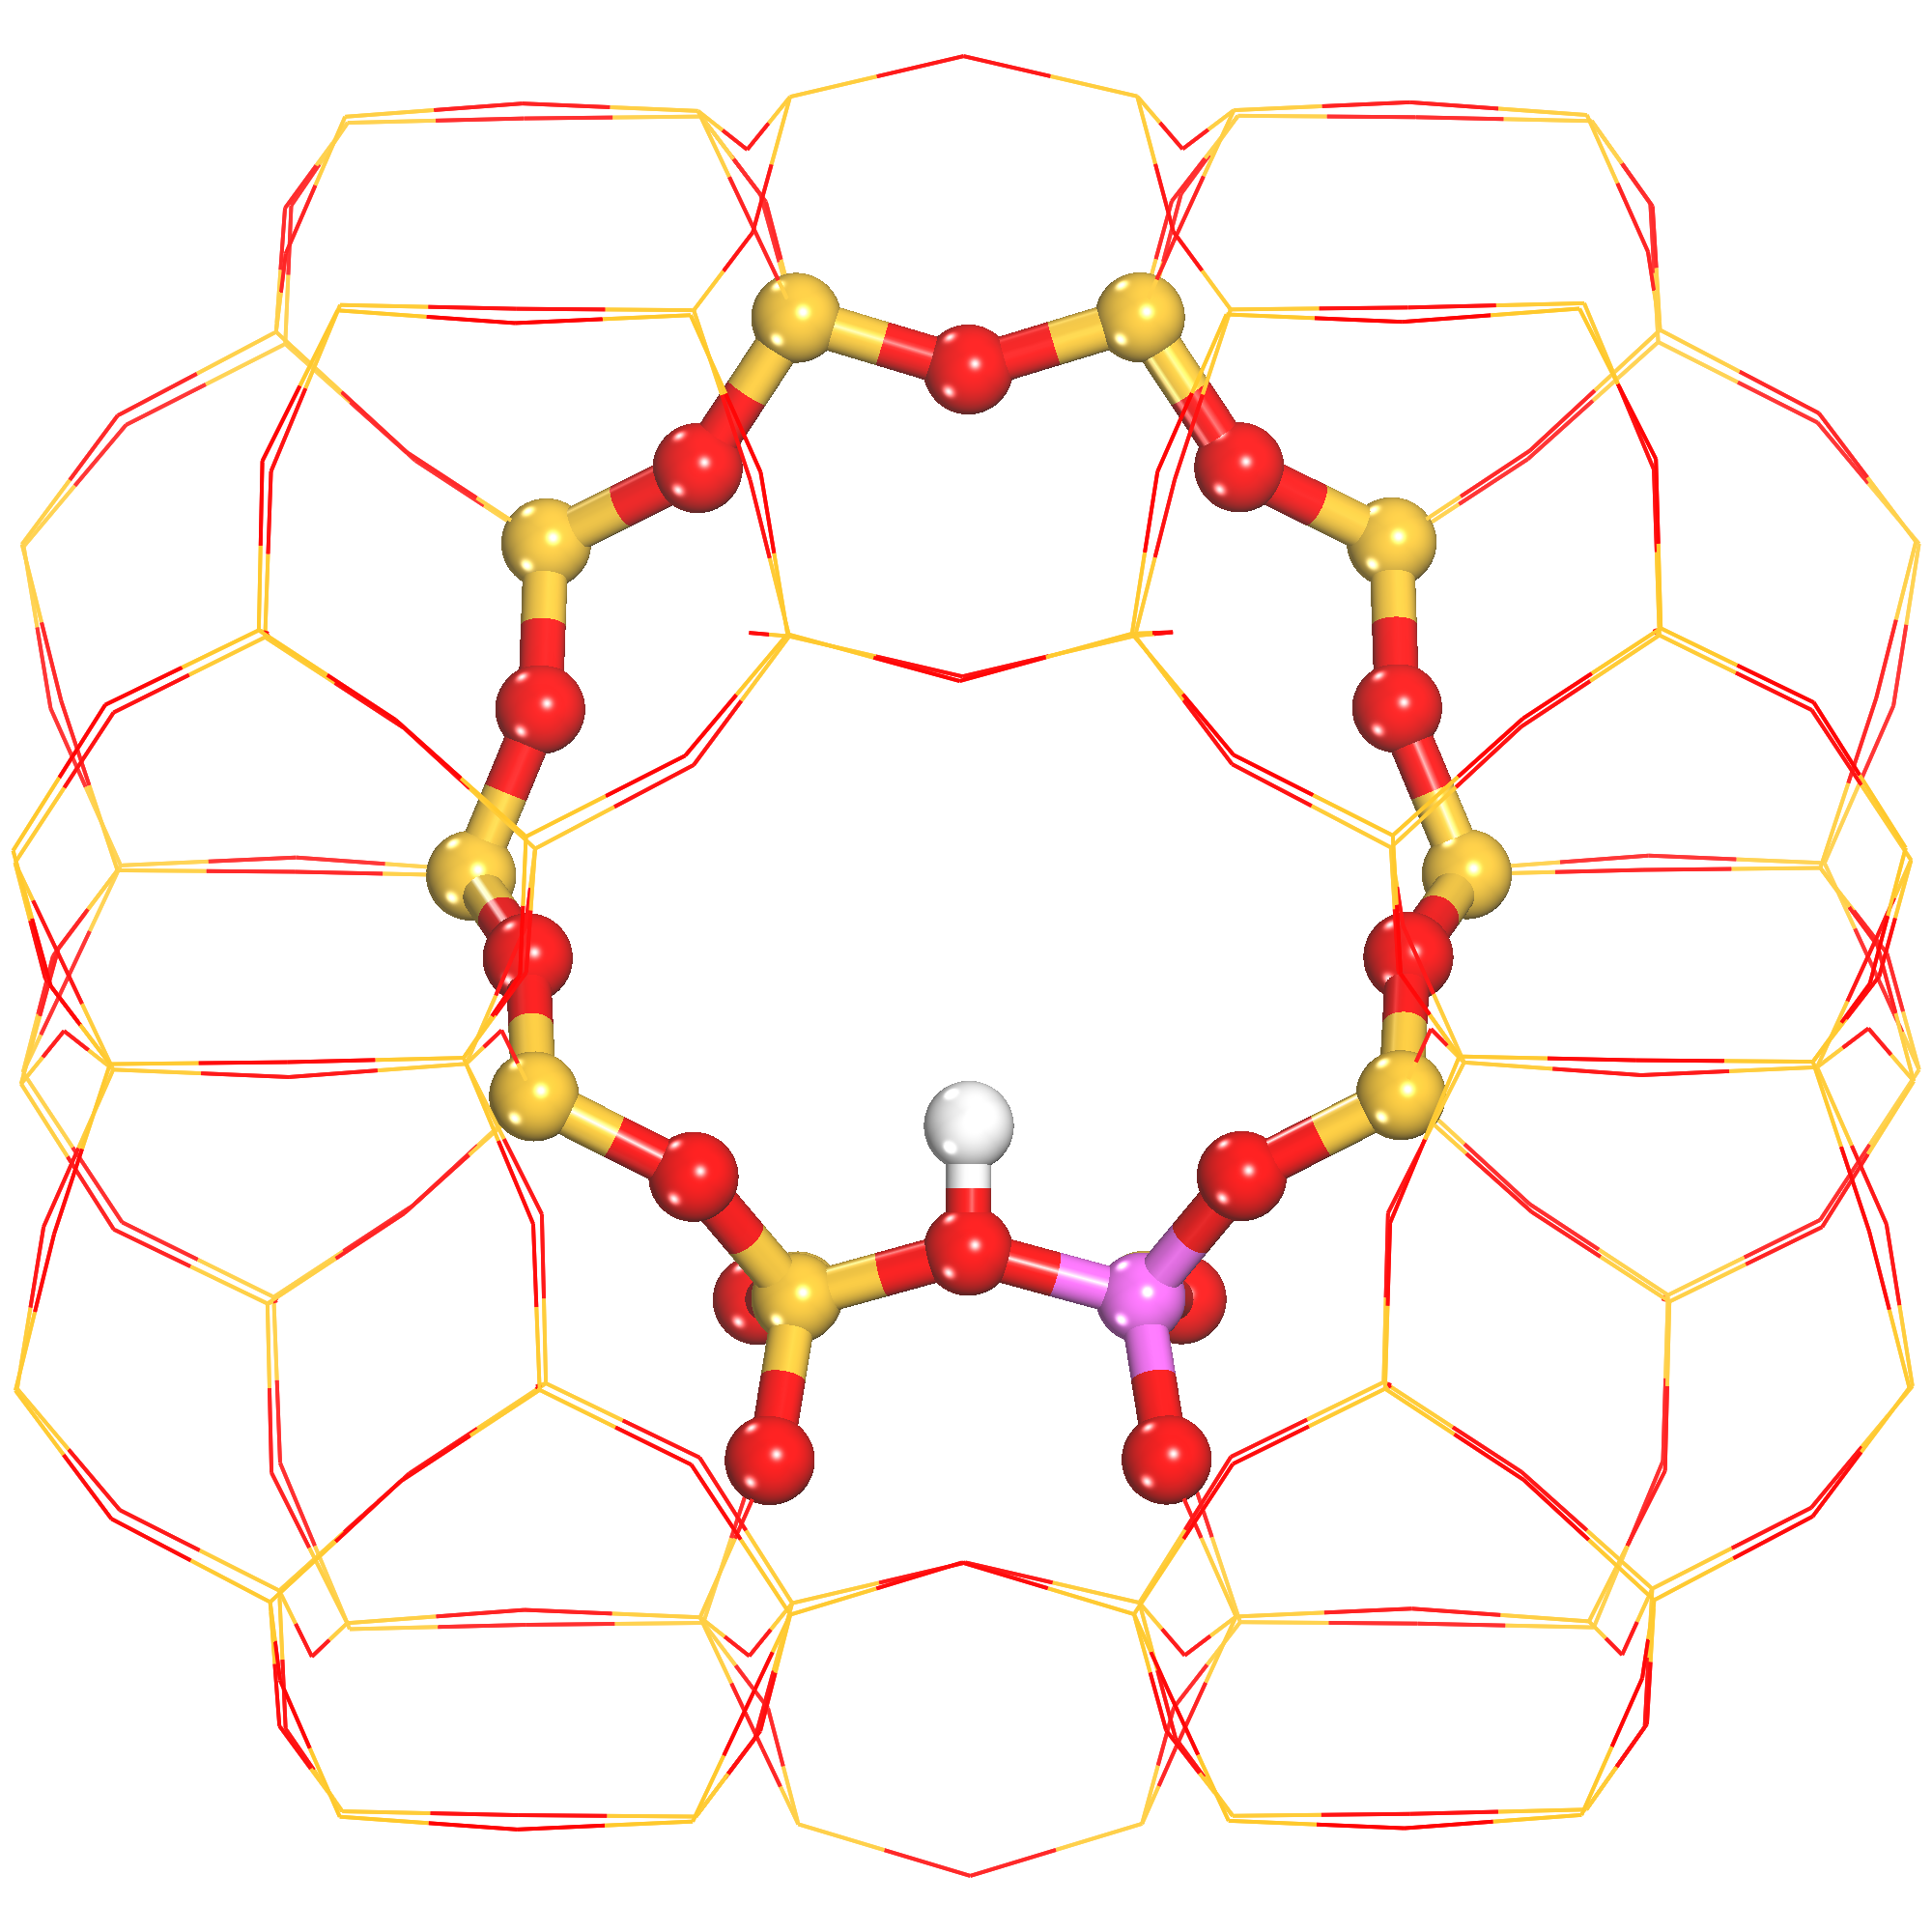
\includegraphics[width=2in]{figure/zigzag.png}
    \end{minipage}%
    }%
    \subfigure[直孔道]{
    \begin{minipage}[t]{0.5\linewidth}
    \centering
    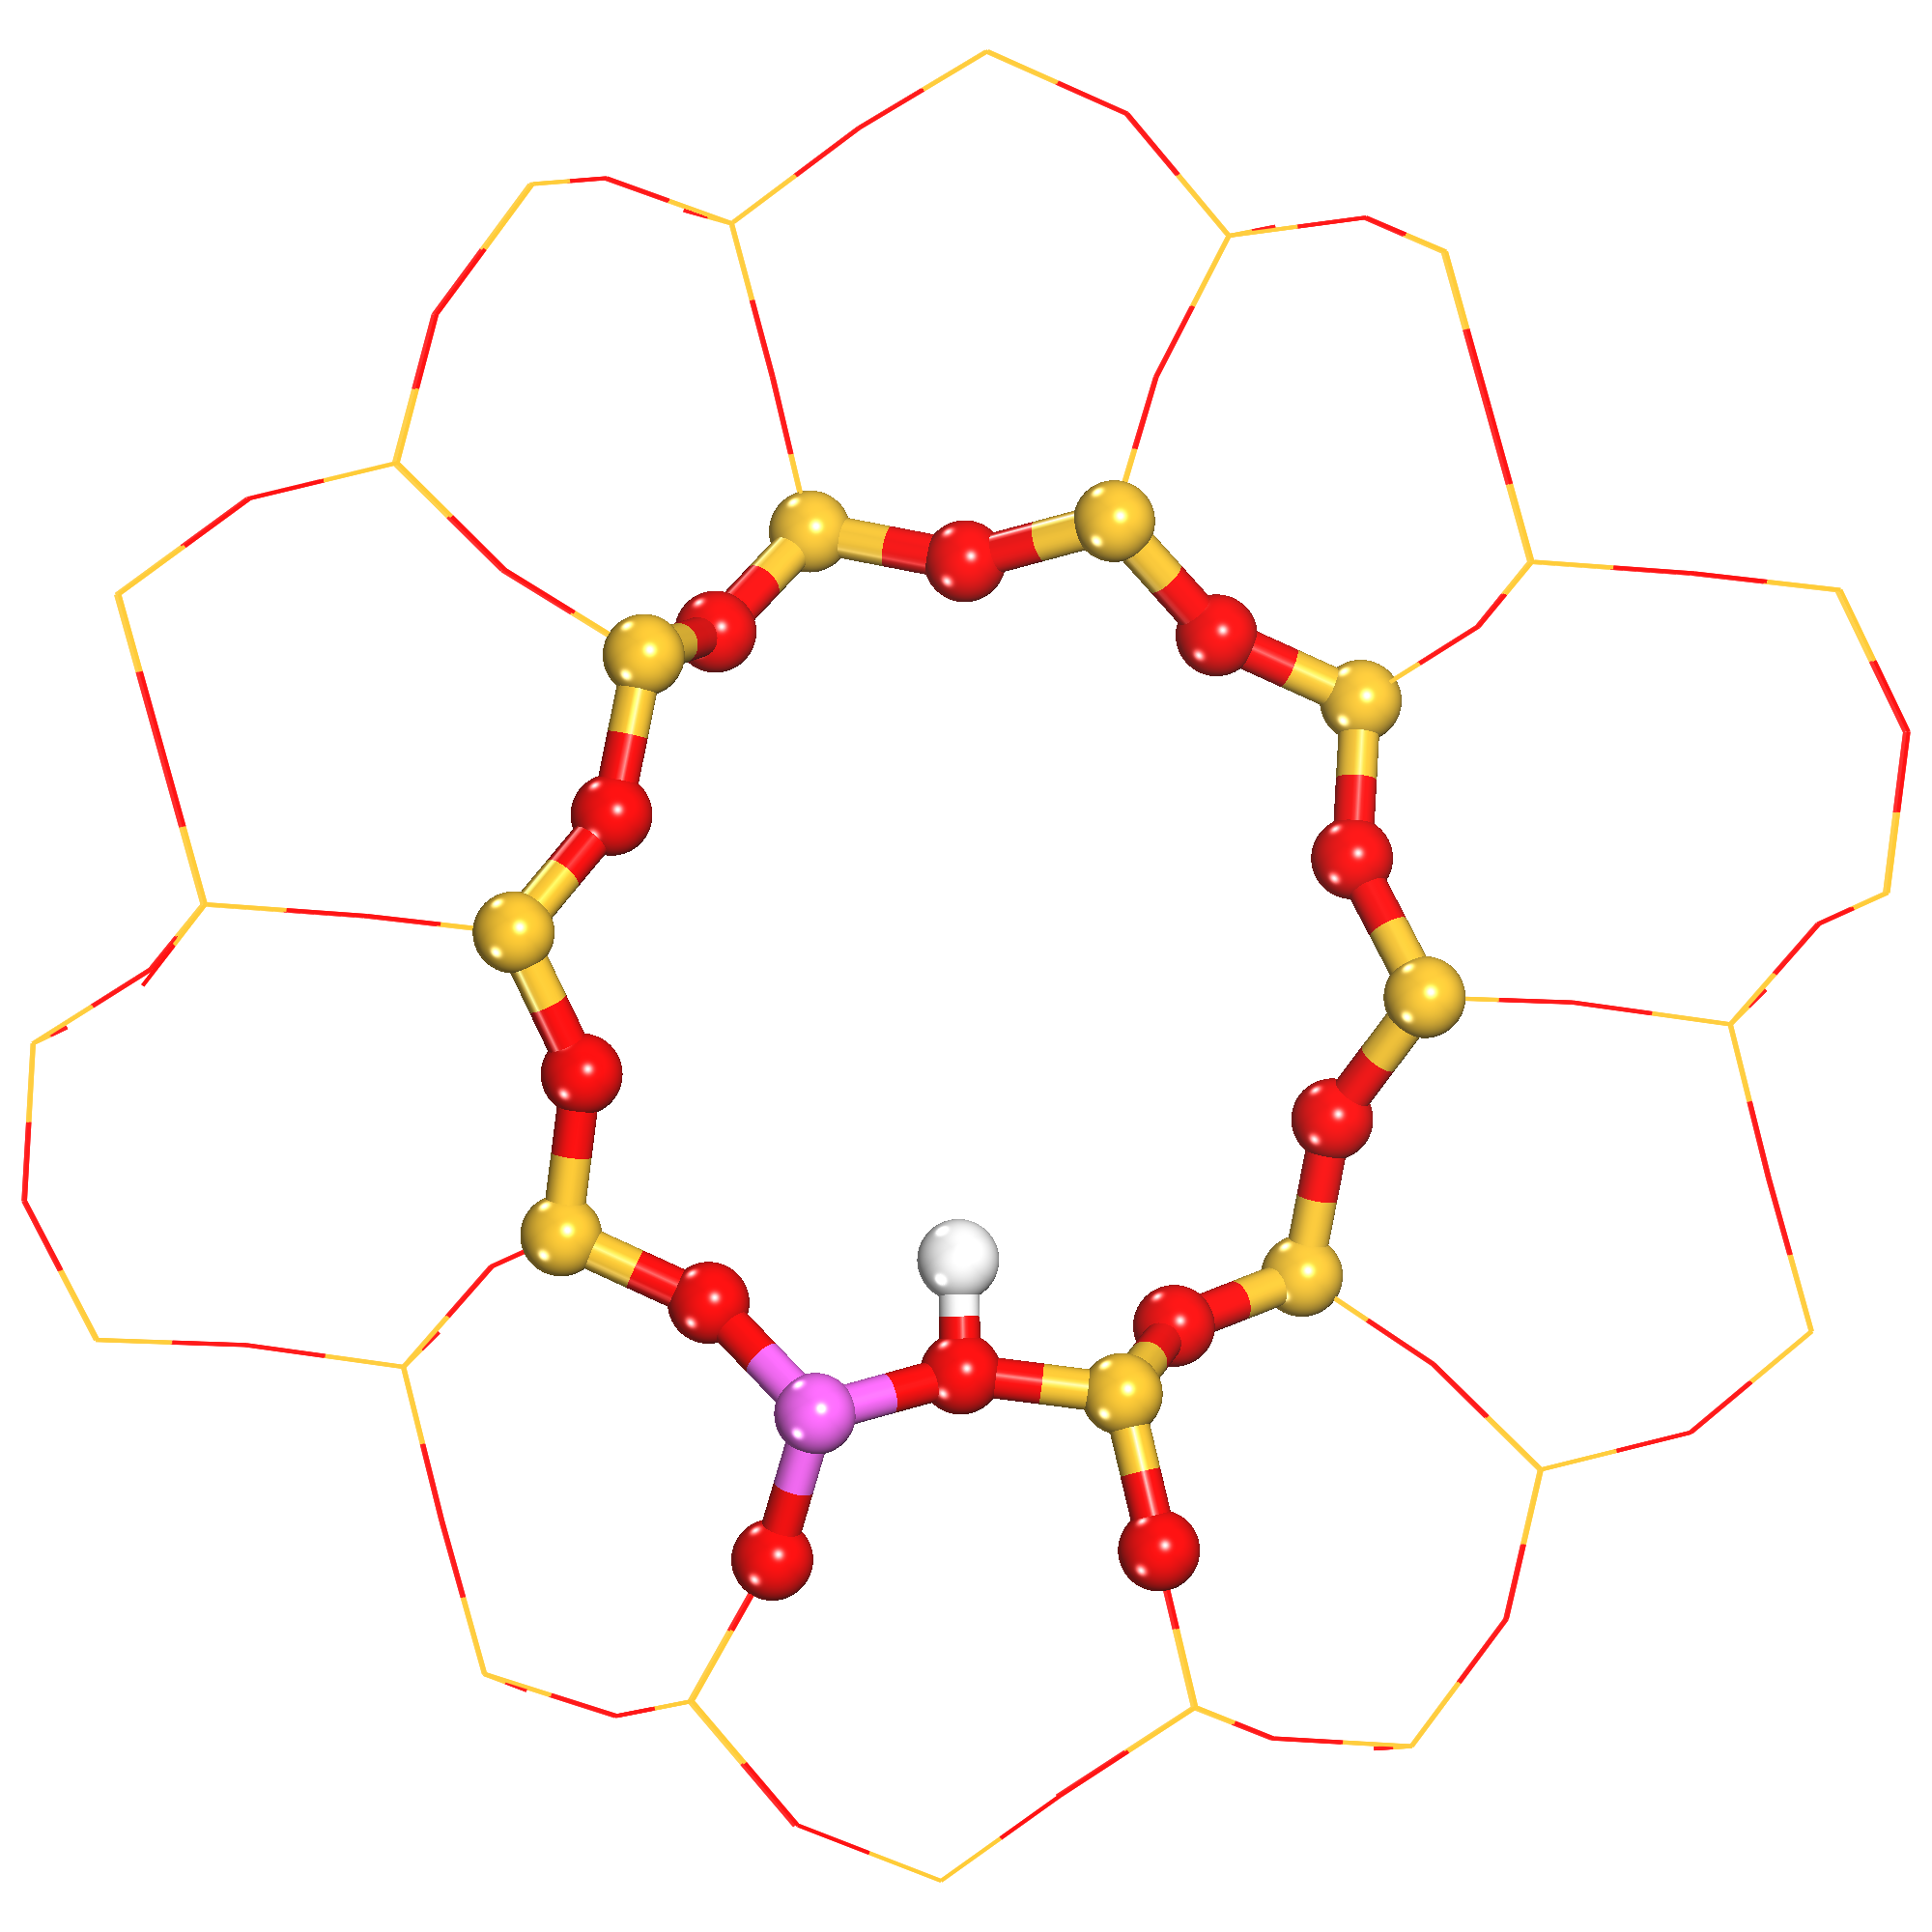
\includegraphics[width=2in]{figure/straight.png}
    %\caption{fig2}
    \end{minipage}%
    }%
    \caption{H-ZSM-5分子筛孔道结构图}
    \label{fig:H-ZSM-5}
\end{figure}
\par{铝原子常被用来取代分子筛骨架上的硅原子,从而形成具有催化活性的质子型或金属离子型分子筛\cite{2013H}。H-ZSM-5分子筛是 ZSM-5 分子筛经过多次铵离子交换处理后,经烘干焙烧得到的 H 型分子筛。H-ZSM-5分子筛的催化活性主要来自Si、Al桥位氧原子质子化所形成的B酸。氢原子除了是反应的活性中心外,也有平衡分子筛电荷的作用。因为H-ZSM-5分子筛在晶体结构、化学组成及物化性质方面具有许多独特性,因此在许多有机催化反应中展现出了优异的催化效果,在工业上得到了越来越广泛地应用\cite{赵振华1985石油化工的新型催化剂——}。}

\subsection{吸附理论}
\subsubsection{吸附简介}
\par{吸附是一种质量传递过程,物体中所有的分子之间都存在互相吸引的力,但在物体表面,内部的分子浓度远大于外部的,表面的分子对物体外部的分子的吸引力没有完全发挥,所以固体的表面可以吸附其他分子。其中吸附剂是具有吸附能力的物质,吸附质是被吸附剂吸附的物质。}
\subsubsection{吸附分类}
\par{吸附按照吸附质与吸附剂间相互作用力性质的差别可以分为化学吸附和物理吸附两大类,具体差异见\reftab{xifu}。}
\begin{table}[htbp]
	\small
	\centering
	\caption{物理吸附和化学吸附对比表}
    \begin{tabular}{p{3cm}<{\centering}p{4cm}<{\centering}p{4cm}<{\centering}}
        \toprule
        吸附类型&物理吸附&化学吸附\\
        \midrule
        作用力&	范德华力	&化学键,电子得失\\
热效应	&近似于凝缩热加润湿热	&近似于化学反应热\\
吸附方式	&单分子层或多分子层	&一般为单分子层\\
解吸结果	&吸附质能还原	&吸附质不能还原\\
吸附过程	&可逆&	不可逆\\
		\bottomrule
	\end{tabular}
	\label{xifu}
\end{table}
\par{本文中的脂肪酸甲酯在 H-ZSM-5 分子筛的吸附属于物理吸附。物理吸附也被称为范德华吸附,它是由吸附剂和吸附质之间的范德华力所引起的。因为任何两个分子间都存在范德华力,所以任何固体表面上都可以发生物理吸附。由于物理吸附是分子间的引力所引起的吸附,所以吸附质与吸附剂之间的作用较弱,于是吸附热较小,吸附和解吸速度也都较快,吸附质容易解吸出来,在一定程度上是可逆的。}
\subsubsection{吸附等温线}
\par{吸附现象的特性包括吸附强度、吸附量、吸附状态等, 而吸附等温线则是宏观地总括这些特性的物理量。吸附等温线是指在一定温度下吸附剂分子在两相的界面上吸附解吸过程达到动态平衡时压力和吸附量之间的关系曲线。}
\par{国际应用化学联合会(IUPAC)根据吸附量随压力的变化将吸附曲线分为以下五种类型:}
\begin{figure}[H]
    \centering

    \subfigure[\uppercase\expandafter{\romannumeral1}型]{
    \begin{minipage}[t]{0.3333\linewidth}
    \centering
    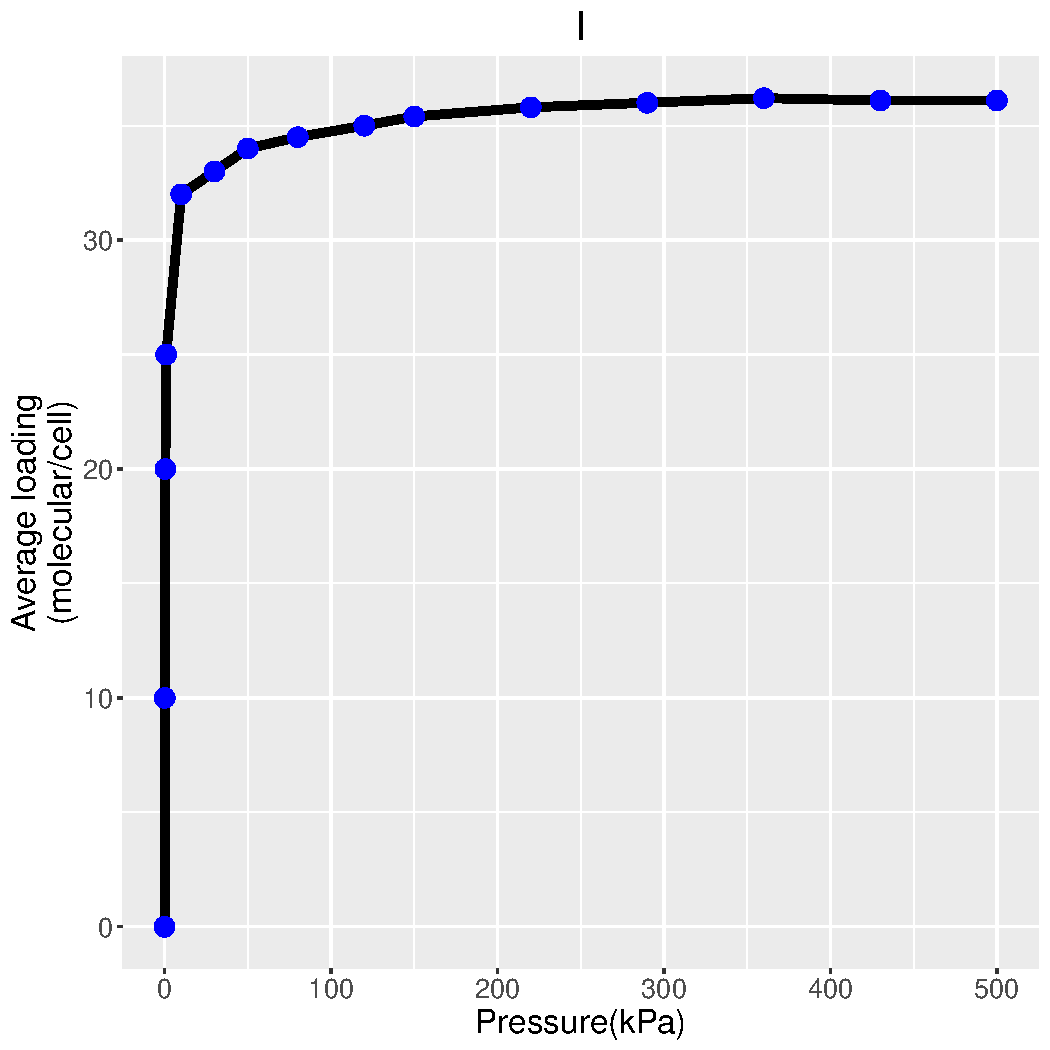
\includegraphics[width=1.8in]{figure/1.pdf}
    %\caption{fig1}
    \end{minipage}%
    }%
    \subfigure[\uppercase\expandafter{\romannumeral2}型]{
    \begin{minipage}[t]{0.3333\linewidth}
    \centering
    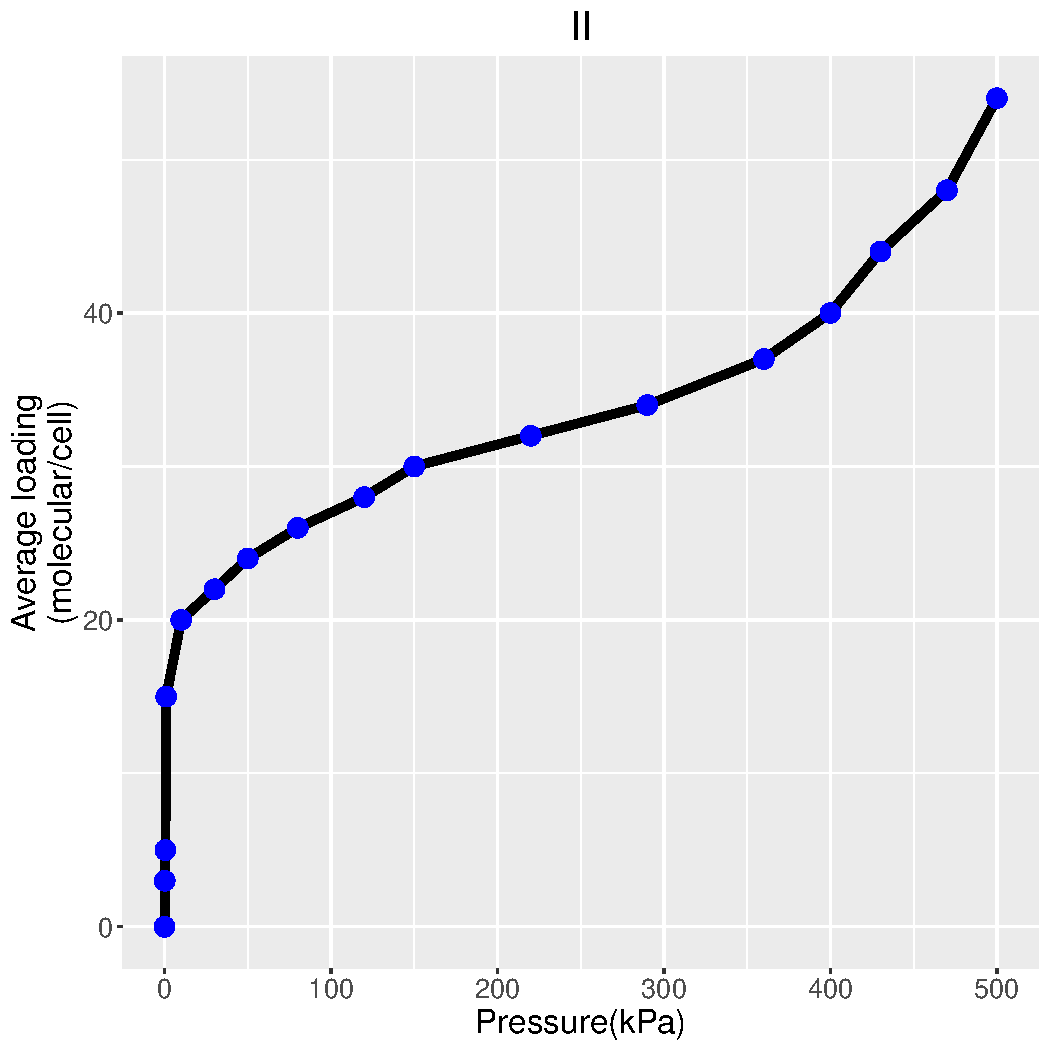
\includegraphics[width=1.8in]{figure/2.pdf}
    %\caption{fig2}
    \end{minipage}%
    }%
    \subfigure[\uppercase\expandafter{\romannumeral3}型]{
    \begin{minipage}[t]{0.3333\linewidth}
    \centering
    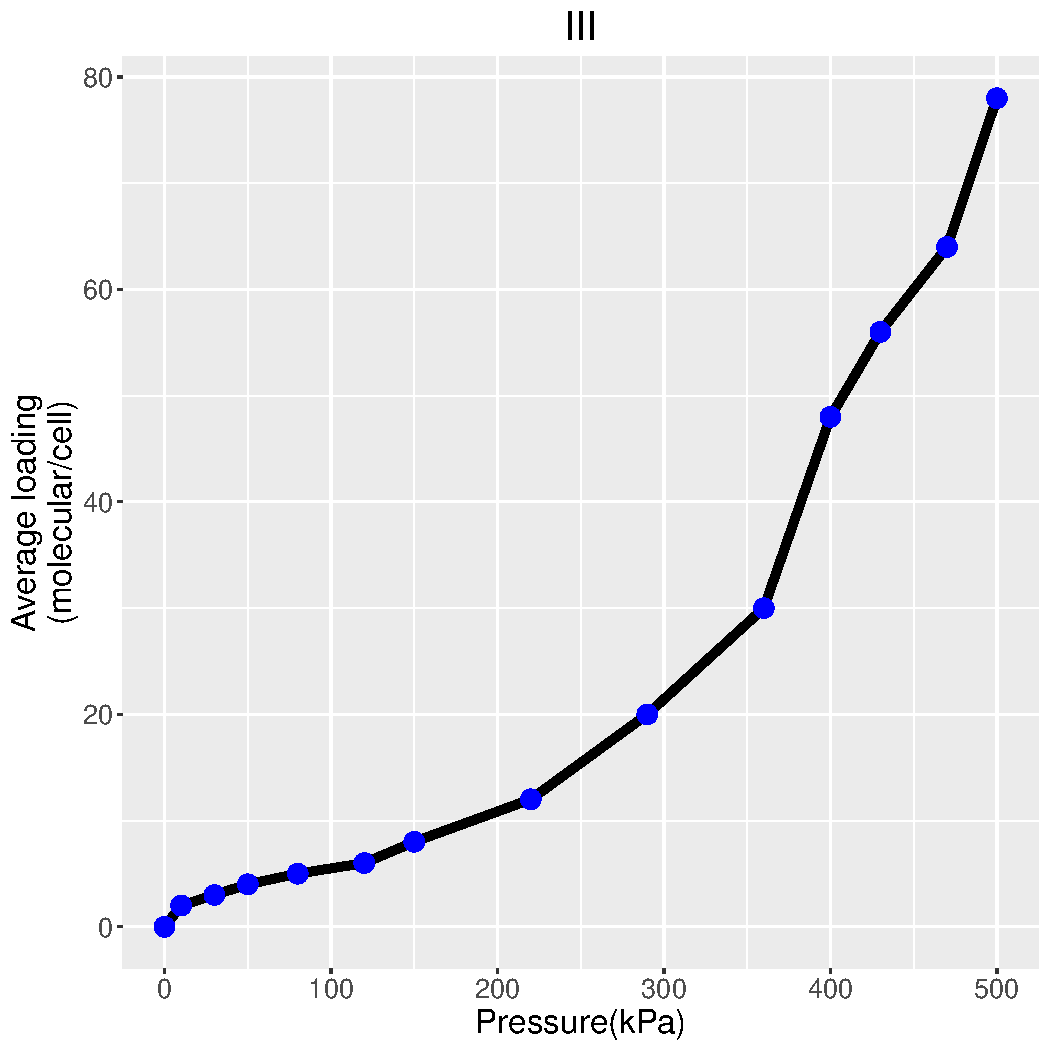
\includegraphics[width=1.8in]{figure/3.pdf}
    %\caption{fig2}
    \end{minipage}%
    }%

    \subfigure[\uppercase\expandafter{\romannumeral4}型]{
    \begin{minipage}[t]{0.3333\linewidth}
    \centering
    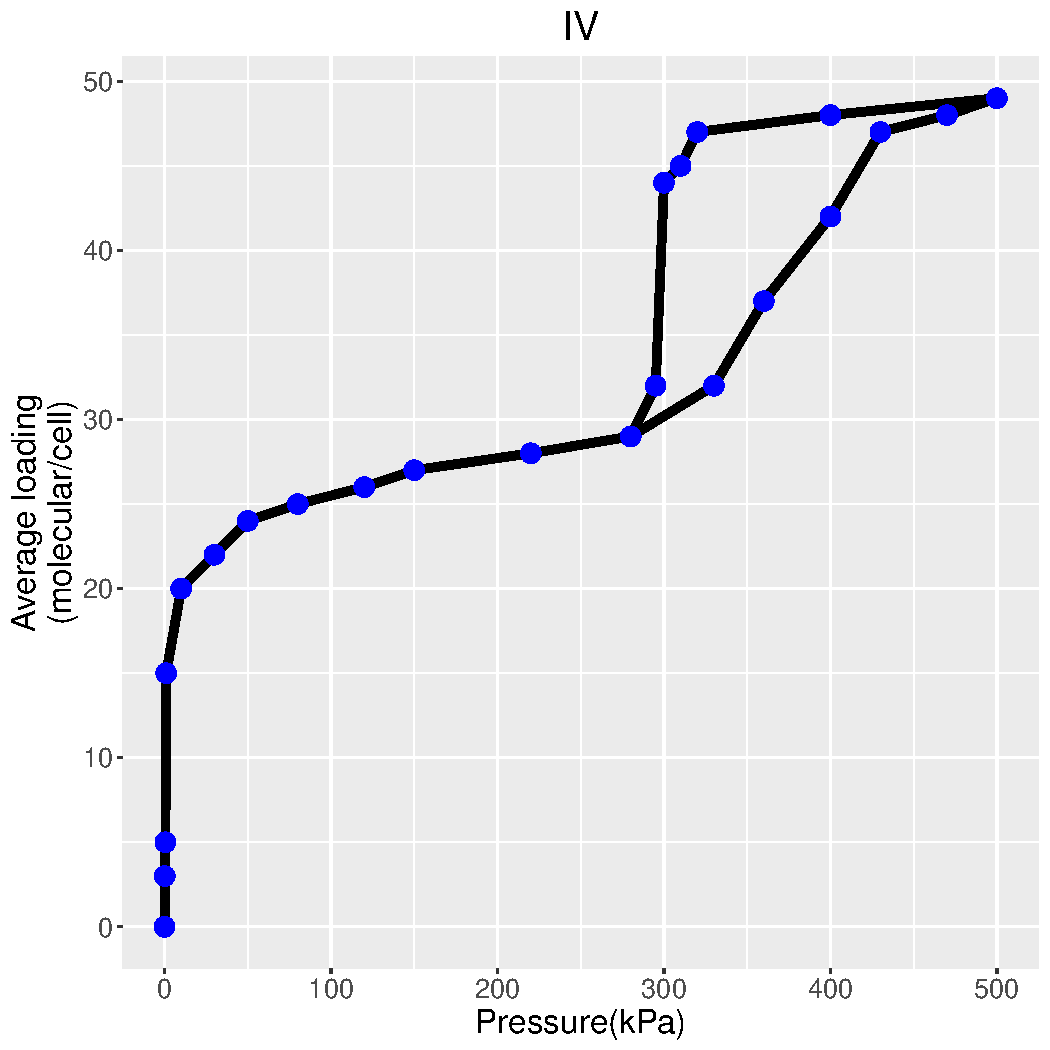
\includegraphics[width=1.8in]{figure/4.pdf}
    %\caption{fig2}
    \end{minipage}%
    }%
    \subfigure[\uppercase\expandafter{\romannumeral5}型]{
    \begin{minipage}[t]{0.3333\linewidth}
    \centering
    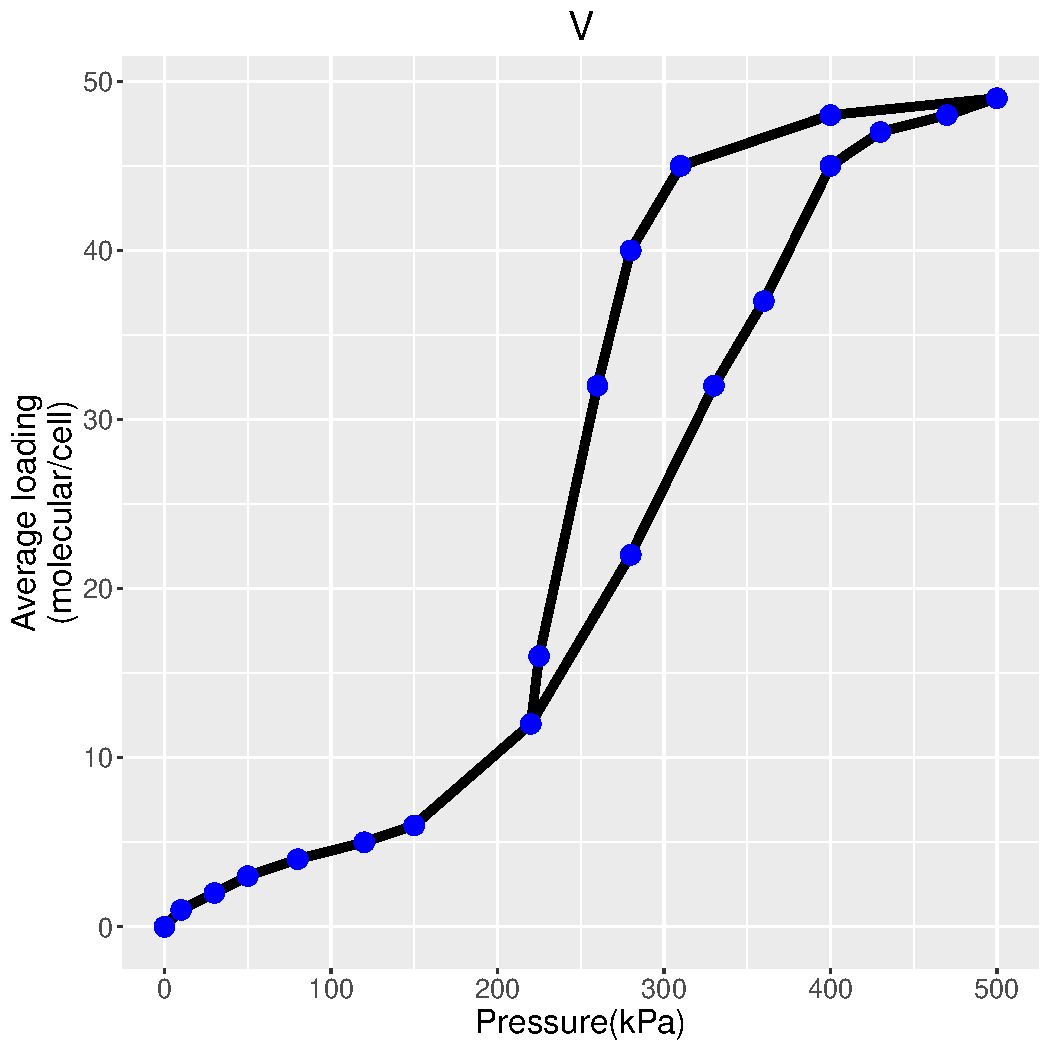
\includegraphics[width=1.8in]{figure/5.pdf}
    %\caption{fig2}
    \end{minipage}%
    }%
    \caption{不同类型的吸附等温线图}
    \label{fig:xifu}
\end{figure}
\subparagraph{Ⅰ型:}
\par{一般反映单分子层可逆吸附,又被称为郎格缪尔等温吸附线。在微孔吸附剂上的吸附等温线一般是这种类型。}
\subparagraph{Ⅱ型:}
\par{一般反映多分子层强吸附。吸附质与吸附剂之间的作用力较大,在较低的压力下吸附量快速增加。拐点处表示单分子层达到吸附饱和,多层吸附随压力的增加逐渐形成,在达到饱和蒸汽压时可近似认为有无限多吸附层。}
\subparagraph{Ⅲ型:}
\par{一般反映多分子层弱吸附。因为吸附质的冷凝热比吸附热还大,所以在高压下吸附速度大于低压下的吸附速度。}
\subparagraph{Ⅳ型和Ⅴ型:}
\par{通常认为是发生了毛细管冷凝后的Ⅱ型和Ⅲ型吸附的变形。}
\subsubsection{郎格缪尔方程}\label{郎格缪尔吸附}
\par{在一定温度下, 吸附质在两相中的浓度关系可用吸附方程式来表示\cite{吴焕领2006吸附等温线的介绍及应用}。朗格缪尔方程是最常用的吸附等温线方程之一,是由物理化学家朗格缪尔 (Langmuir Itying) 根据分子运动理论和一些假定推导出来的,现在被广泛应用于吸附学领域。朗格缪尔认为吸附剂表面的粒子存在向外的剩余价力,它可以吸附气体分子,而这种剩余价力的作用范围与分子直径相当,所以吸附剂表面只能发生单分子层吸附。}
\par{郎格缪尔吸附存在四个假设:}
\begin{enumerate}
    \item 吸附剂的吸附位点只存在于表面,且每个吸附位点只能吸附单个分子;
    \item 吸附剂表面是均匀的,表面上各位点发生吸附的吸附热相同;
    \item 吸附质分子之间的作用力远小于吸附质与吸附剂间的作用力,可以忽略;
    \item 吸附的同时也存在脱附,吸附平衡是动态平衡。
\end{enumerate}
\par{根据上面的假设,可以推导出朗格缪尔吸附方程:}
\par{对于任意吸附过程,均存在如下平衡:}
\begin{equation}
    X(g)+Y(s) \xleftrightarrow[k_{-1}]{k_1} X Y
\end{equation}
\par{式中:$X(g)$ 表示吸附质;$Y(s)$ 表示吸附剂; $k_1$为吸附速率常数;$k_{-1}$ 为解吸速率常数。}
\par{吸附速率表示为:}
\begin{equation}
    V_{1}=k_{1} P(1-\theta) N
\end{equation}
\par{式中:$V_{1}$表示吸附速率;$P$ 为压力; $\theta$为覆盖率; $N$为吸附数。}
\par{解吸速率表示为:}
\begin{equation}
    V_{-1}=k_{-1} \theta N
\end{equation}
\par{式中:$V_{-1}$ 为解吸速率。}
\par{当达到饱和吸附量时,吸附和解吸达到动态平衡,即$V_{1}=V_{-1}$,所以:}
\begin{equation}
    \theta=\frac{b P}{1+b p}
\end{equation}
\par{式中:}
\begin{equation}
    b=\frac{k_{1}}{k_{-1}}
\end{equation}
\par{因为假设吸附为单分子层吸附,而$\theta$为覆盖率,故设:}
\begin{equation}
    \theta=\frac{V_{\mathrm{m}}}{V_{\mathrm{m}^{a}}}
\end{equation}
\par{式中:$V_{\mathrm{m}}$为平衡吸附量;$V_{\mathrm{m}^{a}}$ 为饱和吸附量。}
\par{故:}
\begin{equation}
    V_{\mathrm{m}}=V_{\mathrm{m}^{\mathrm{a}}} \frac{b P}{1+b P}
\end{equation}
\subsection{扩散理论}
\subsubsection{扩散简介}
\par{物质分子从浓度高的地方向浓度低的地方进行转移,直到体系浓度均匀分布的现象叫扩散\cite{2014半无限大体广义电磁热弹扩散问题的动态响应}。扩散由不同区域之间的温度差或者浓度差引起,可以发生在一种或几种物质在同一相态或不同相态之间,直到同一相态内各区域各种物质的浓度均匀或者两相间各种物质的浓度平衡为止。}

\subsubsection{菲克定律}
\par{菲克定律描述的是化工“三传一反”中的质量传递现象。菲克定律是指在不依靠宏观的混合作用发生的传质现象时,描述分子扩散过程中质量通量与浓度梯度之间关系的定律。它包括两个内容:}
\subparagraph{菲克第一定律:}
\par{在单位时间内通过垂直于扩散方向的单位截面积的扩散流量与该截面处的浓度梯度成正比。公式表达为:}
\begin{equation}
    J=-D \dfrac{\partial C}{\partial X}
    \end{equation}
\par{式中:$J$为扩散通量;$D$为扩散系数;$C$为扩散物质的体积浓度;$\dfrac{\partial C}{\partial X} $为浓度梯度;负号表示扩散方向与浓度梯度的方向相反。}
\subparagraph{菲克第二定律:}
\par{在非稳态扩散过程中,$X$ 处的浓度随时间的变化率$\dfrac{\partial C}{\partial t}$ 等于该处的扩散通量随距离变化率的相反数。公式表达为:}
\begin{equation}
    \frac{\partial C}{\partial t}=\frac{\partial \frac{\partial C}{\partial X}}{\partial X}\xrightarrow{\mbox{D不随X变化}}D \frac{\partial^{2} C}{\partial X^{2}}
\end{equation}
\subsubsection{扩散系数}
\par{扩散系数(菲克定律中的$D$)是指在单位时间单位浓度梯度下,沿扩散方向且垂直于单位面积所传递的质量或物质的量。扩散系数主要受扩散物质的物性、压力和温度的影响。}
\par{多年来众多学者都致力于研究扩散物质在分子筛中的扩散机理以及如何测定扩散系数。目前实验测定扩散系数有多种方法:Tezel\cite{tezel1991effect}等人用重量法测定了氮气在分子筛上的扩散动力学;Zhu\cite{zhu2004concentration}等人采用零长度色谱法研究了异丁烷在分子筛上的脱附;卢洪\cite{卢洪2000炭分子筛上氧、氮吸附特性的实验测定}等人用气相色谱法测定了氮气和氧气在分子筛上的扩散系数。而随着计算机技术的发展,分子模拟技术已经被广泛应用在分子筛上的扩散行为的研究\cite{陈玉平2007烷烃在分子筛孔中吸附和扩散的分子模拟,袁帅2011芳烃、环烷烃分子在,杨超2006甲苯歧化反应物与产物在}。}
\subsection{分子模拟理论和方法简介}
\par{分子模拟所依据的理论主要包括经典力学(CM)和量子力学(QM)。常用的经典力学方法主要有:分子力学方法(MM)、蒙特卡罗方法(MC)和分子动力学方法(MD)。常用的量子力学方法有:半经验算法(Semi-empirical Method),从头算方法(Ab initio Method)以及密度泛函理论(Density Functional Theory)\cite{刘丹2004分子模拟在分子筛催化研究中的应用}。}
\par{与实验相比,利用计算机研究化学现象的方法有下列几项优点\cite{分子模拟的理论与实践}:}
\begin{enumerate}
    \item 降低研究成本;
    \item 增加安全性;
    \item 可研究极快速的反应或变化;
    \item 准确度较高;
    \item 增加对问题的了解。
\end{enumerate}
\par{本文采用的方法主要有分子力学、分子动力学、蒙特卡洛法和密度泛函理论。通过密度泛函理论和分子力学可以得到吸附分子和分子筛的几何优化构象;通过蒙特卡洛法可以得到吸附等温线、吸附热、吸附位点以及吸附质在分子筛中的分布情况;通过分子动力学可得到扩散轨迹和扩散系数。}
\par{下面对所采用的方法以及模拟原理进行简单的介绍。}
\subsubsection{分子力学}
\par{分子力学是在原子、分子水平上用力场解决问题的非量子力学方法\cite{王艺峰2003高分子材料模拟中的分子力学法和力场}。根据波恩-奥本海默近似原理,可以将分子中电子运动的能量忽略,所以体系的能量就是原子核位置的函数。分子力学中的力场中的许多参数可以通过量子力学计算或者实验方法得到,从而避开了考虑电子结构和运动的细节,所以利用分子力学可以计算庞大且复杂的分子的稳定构象、热力学特性和振动光谱等性质\cite{分子模拟的理论与实践}。与量子力学相比,分子力学简单并且可以快速得到分子的各种性质。}
\par{在分子模拟中,合适的力场对于模拟结果的准确性起着决定性作用,它是分子力学方法的核心和关键。通过选取合适的力场就可以计算出分子各种构象的势能,而势能最小的构象就是最稳定的构象。求取势能最低点的过程被称为能量最小化,所得到的构象被称为几何优化构象,它是计算分子物性的基础。本文采用了COMPASS\RNum{2}力场进行模拟。COMPASS\RNum{2}力场能够模拟小分子与高分子,一些金属离子、金属氧化物与金属。在计算有机与无机体系时,采用分类别处理的方式,不同的类别采用不同的模型,即使在计算两种类别的混合体系时,仍然能够采用合理的模型描述\cite{梁太宁2001分子力场},所以COMPASS\RNum{2}力场非常适合本文的脂肪酸甲酯与分子筛体系。其中共价键模型的形式如下:}
\begin{align}
    U &=U_{\mbox{\tiny 键合项}}+U_{\mbox{\tiny 非键合项}}\notag\\
      &=U_{\mbox{\tiny 键合项}}+U_{i, j}+U_{elec}
\end{align}
\begin{align}
    U_{\mbox{\tiny 键合项}} &= U_{b}+U_{\theta}+U_{\phi}+U_{\chi}+U_{cross}\notag\\
      &=\sum_{b}\left[k_{2}\left(b-b_{0}\right)^{2}+k_{3}\left(b-b_{0}\right)^{3}+k_{4}\left(b-b_{0}\right)^{4}\right]\notag\\
      &+\sum_{\theta}\left[k_{2}\left(\theta-\theta_{0}\right)^{2}+k_{3}\left(\theta-\theta_{0}\right)^{3}+k_{4}\left(\theta-\theta_{0}\right)^{4}\right]\notag\\
      &+\sum_{\phi}\left[k_{1}(1-\cos \phi)+k_{2}(1-\cos 2\phi)+k_{3}(1-\cos 3\phi)\right]\notag\\
      &+\sum_{\chi} k_{2} \chi^{2}+\sum_{b, b^{\prime}} k\left(b-b_{0}\right)\left(b-b_{0}^{\prime}\right)+\sum_{b, \theta} k\left(b-b_{0}\right)\left(\theta-\theta_{0}\right)\notag\\
      &+\sum_{b, \phi} \left(b-b_{0}\right)\left[k_{1} \cos \phi+k_{2} \cos 2 \phi+k_{3} \cos 3 \phi\right]\notag\\
      &+\sum_{b^{\prime}, \phi} \left(b^{\prime}-b_{0}^{\prime}\right)\left[k_{1} \cos \phi+k_{2} \cos 2 \phi+k_{3} \cos 3 \phi\right]\notag\\
      &+\sum_{\theta, \phi} \left(\theta+\theta_{0}\right)\left[k \cos \phi+k \cos 2 \phi+k \cos 3 \phi\right]\notag\\
      &+\sum_{\theta^{\prime}, \theta} k\left(\theta^{\prime}-\theta_{0}^{\prime}\right)\left(\theta-\theta_{0}\right)+\sum_{\theta^{\prime}, \theta, \phi} k\left(\theta^{\prime}-\theta_{0}^{\prime}\right)\left(\theta-\theta_{0}\right)\cos \phi
\end{align}
\begin{equation}
    U_{elec}=\sum_{i, j} \frac{q_{i} q_{j}}{r_{i j}}
\end{equation}
\begin{equation}
    U_{i, j}=\sum_{i, j} \varepsilon_{ij}\left[2\left(\frac{r_{i j}^{0}}{r_{i j}}\right)^{9}-3\left(\frac{r_{i j}^{0}}{r_{i j}}\right)^{6}\right]
\end{equation}

\par{式中:$U_{i, j}$是范德华能;$U_{elec}$是库伦能;$U_{b}$是键伸缩能;$U_{\theta}$是键角弯曲能;$U_{\phi}$是键扭转能;$U_{\chi}$是键角面外弯曲能;$U_{cross}$是相互耦合能。}
\par{将分子中各原子核的位置参数带入COMPASS\RNum{2}力场即可得到体系的总能量,再通过最速下降法、共轭梯度法、牛顿拉森法等方法求得该势能函数的最小值和对应的位置参数。通过位置参数,即可得到该分子的几何优化构象。}
\subsubsection{密度泛函理论}
\par{量子力学是以分子中电子的非定域化为基础,认为体系内粒子运动满足薛定谔方程,一切电子的行为以其波函数表示。通过分析分子所表现的性质与其微观结构参数(如电荷密度、轨道、能级等)的关系,而后再根据性质来优化模型结构。理论上讲,量子力学方法几乎可以得到关于分子的一切信息与性质,且结果与实验的结果往往相当吻合。}
\par{密度泛函理论是一种通过研究物质结构统计性的理论,既可以通过量子力学的密度泛函理论研究微观结构,也可以通过统计力学的密度泛函理论研究宏观结构。密度泛函理论都是以密度分布$\rho(r)$作为变量,然后构建密度泛函,它不是某个特定位置的函数,而是函数在整个变量空间中的变化。其中量子力学的密度泛函理论是通过电子的密度分布$\rho(r)$代替波函数$\Psi(\tau)$作为变量,然藏构筑能量的密度泛函,最后应用薛定谔方程求解\cite{密度泛函理论}。薛定谔方程如\refequ{xue1}和\refequ{xue2}所示。}
\begin{equation}\label{xue1}
    -\frac{\hbar^{2}}{2 \mu}\left(\frac{\partial^{2} \Psi}{\partial x^{2}}+\frac{\partial^{2} \Psi}{\partial y^{2}}+\frac{\partial^{2} \Psi}{\partial z^{2}}\right)+U(x, y, z) \Psi=i \hbar \frac{\partial \Psi}{\partial t}
\end{equation}
\begin{equation}\label{xue2}
    -\frac{\hbar^{2}}{2 \mu} \nabla^{2} \Psi+U \Psi=E \Psi
\end{equation}
\par{通过求解薛定谔方程即可求得波函数$\Psi$对应的本征值$E$,即可求得能量。通过比较不同波函数的本征值就可以求得最低能量,而该波函数的坐标参数所对应的结构即是几何优化构象。}
\subsubsection{蒙特卡洛法}
\par{蒙特卡洛方法又被称为随机模拟方法,是一种对构建好的概率模型重复进行大数量的统计模拟,其核心是一种统计方法。在一定系综条件下, 将体系内粒子进行随机的转动、位移或在两相间转移位置,然后运用统计热力学理论进行统计平均,使结果逐渐趋近于平衡时的玻尔兹曼分布,以此获得体系的宏观性质。所以理论上来说,只要有足够多的粒子,就能得到期望的宏观量。该方法最大的优势在于其收敛条件不受问题维数的影响,但由于粒子的位移是计算机随机赋予的,只能在大数量实验结果下反应概率问题,并不能代表粒子的真实运动过程,所以不能用于模拟传递性质\cite{分子模拟技术在石油相关领域的应用}。}
\par{蒙特卡洛方法的模拟过程一般分为如下几步\cite{分子模拟的理论与实践}:}
\begin{enumerate}
    \item 通过随机数发生器生成一个初始的分子构型。
    \item 将这个分子构型中原子的坐标做无规律的改变,生成一个新的分子构型。
    \item 计算出新的分子构型的能量。
    \item 比较原分子构型和新的分子构型的能量大小,判断是否采用新构型。
    \begin{enumerate}[label=(\alph*),leftmargin=2em]
        \item 假如新的分子构型能量小于原分子构型的能量,则接受新的分子构型,并使用这个构型重复再做下一次迭代。
        \item 假如新的分子构型能量大于原分子构型的能量,则计算出玻尔兹曼因子,并生成一个随机数。假如这个随机数大于所计算出的玻尔兹曼因子,则舍弃这个构型,重新计算。若这个随机数小于所计算出的玻尔兹曼因子,则接受这个构型,使用这个构型重复再做下一次迭代。
    \end{enumerate}
    \item 如此进行迭代计算,直至最后得到低于所给能量条件的分子构型为止。
\end{enumerate}
\par{计算吸附性能时采用的是巨正则系综(GCMC),这代表体系的粒子数N不固定,但体系的体积V、化学势μ和温度T不变。利用达到平衡时,吸附剂表面的吸附质的温度和化学势与吸附剂外的相等,从而可以研究在固定温度和压力下吸附质分子在吸附剂内的吸附特性。}
\subsubsection{分子动力学}\label{分子动力学}
\par{分子动力学模拟是一种依靠经典力学来计算经典多体系的平衡过程以及传递性质的模拟方法\cite{分子模拟方法及模拟软件在高分子材料中的应用}。与蒙特卡洛方法相比,分子动力学中的模拟中系统中粒子的运动有正确的物理依据。而且此方法的计算精度性高,可同时获取系统的动态与热力学统计资料。}
\par{分子动力学模拟过程通常遵循以下六个步骤\cite{烷烃分子在MCM-41中吸附和扩散的分子模拟}:}
\begin{enumerate}
    \item 将体系中的粒子看作质点;
    \item 将体系中的所有质点根据玻尔兹曼分布指定初始速度以及初始位置;
    \item 根据所选力场,计算每个质点的势能,确定每个粒子在体系中受到的力;
    \item 根据经典力学,求解运动方程;
    \item 在指定模拟时间内重复步骤(3)和(4);
    \item 将计算结果平均应用到整个体系,确定体系的宏观特性。
\end{enumerate}
\par{通过上面的计算步骤,可以得到体系中所有粒子的扩散轨迹,这些轨迹可以反映出系统中粒子的真实运动状态。以$\vec r_{i}(t)$表示时间$t$时粒子i的位置,粒子位移平方的平均值称为均方位移(MSD),即:}
\begin{equation}
    \mathrm{MSD}=R(t)=\left\langle|\vec{r}(t)-\vec{r}(0)|^{2}\right\rangle
\end{equation}
\par{式中:尖括号表示平均值。}
\par{根据统计的原理,只要有足够多的粒子,足够长的计算时间,系统的任一瞬间都可以当作时间的零点,而所计算的平均值应该相同。假设分子动力学计算共存储了n步轨迹,各步的位置向量分别是$\vec r(1)$、$\vec r(2)$、$\vec r(1)$、……和$\vec r(n)$。在计算均方位移时,每次计算$R(t)$取$n/2$组数据的平均。将轨迹分为:}
$$
\vec{r}(1)\mbox{,}\vec{r}(2)\mbox{,……,}\vec{r}(n / 2)\quad\mbox{及}\quad\vec{r}(n / 2+1)\mbox{,}\vec{r}(n / 2+2)\mbox{,……,}\vec{r}(n)
$$
\par{假设每步的时间间隔为$\delta t$,因为任一瞬间都可以视为零点,所以均方位移为:}
\begin{align}\label{equ:MSD}
    R(\delta t)&=\frac{|\vec{r}(2)-\vec{r}(1)|^{2}+|\vec{r}(3)-\vec{r}(2)|^{2}+\cdots+|\vec{r}(n / 2+1)-\vec{r}(n / 2)|^{2}}{n / 2}\notag\\
    R(2 \delta t)&=\frac{|\vec{r}(3)-\vec{r}(1)|^{2}+|\vec{r}(4)-\vec{r}(2)|^{2}+\cdots+|\vec{r}(n / 2+2)-\vec{r}(n / 2)|^{2}}{n / 2}\notag\\
    &\dots\notag\\
    R(m \delta t)&=\frac{|\vec{r}(m+1)-\vec{r}(1)|^{2}+|\vec{r}(m+2)-\vec{r}(2)|^{2}+\cdots+|\vec{r}(m+n / 2)-\vec{r}(n / 2)|^{2}}{n / 2}\notag\\
    &\dots\notag\\
    R(n \delta t / 2)&=\frac{|\vec{r}(n / 2+1)-\vec{r}(1)|^{2}+|\vec{r}(n / 2+2)-\vec{r}(2)|^{2}+\cdots+|\vec{r}(n)-\vec{r}(n / 2)|^{2}}{n / 2}
\end{align}
\par{\refequ{equ:MSD}是计算一个粒子均方位移的公式,如果要计算系统中所有粒子的均方位移则需要再对粒子数进行平均。\reffig{fig:MSD}展示了LJ势能下的系统的均方位移与时间的曲线。由\reffig{fig:MSD}可知:当时间值很小时,MSD以对数形式增加;当时间值很大时,曲线近似为一条直线。}
\begin{figure}[H]
    \centering
    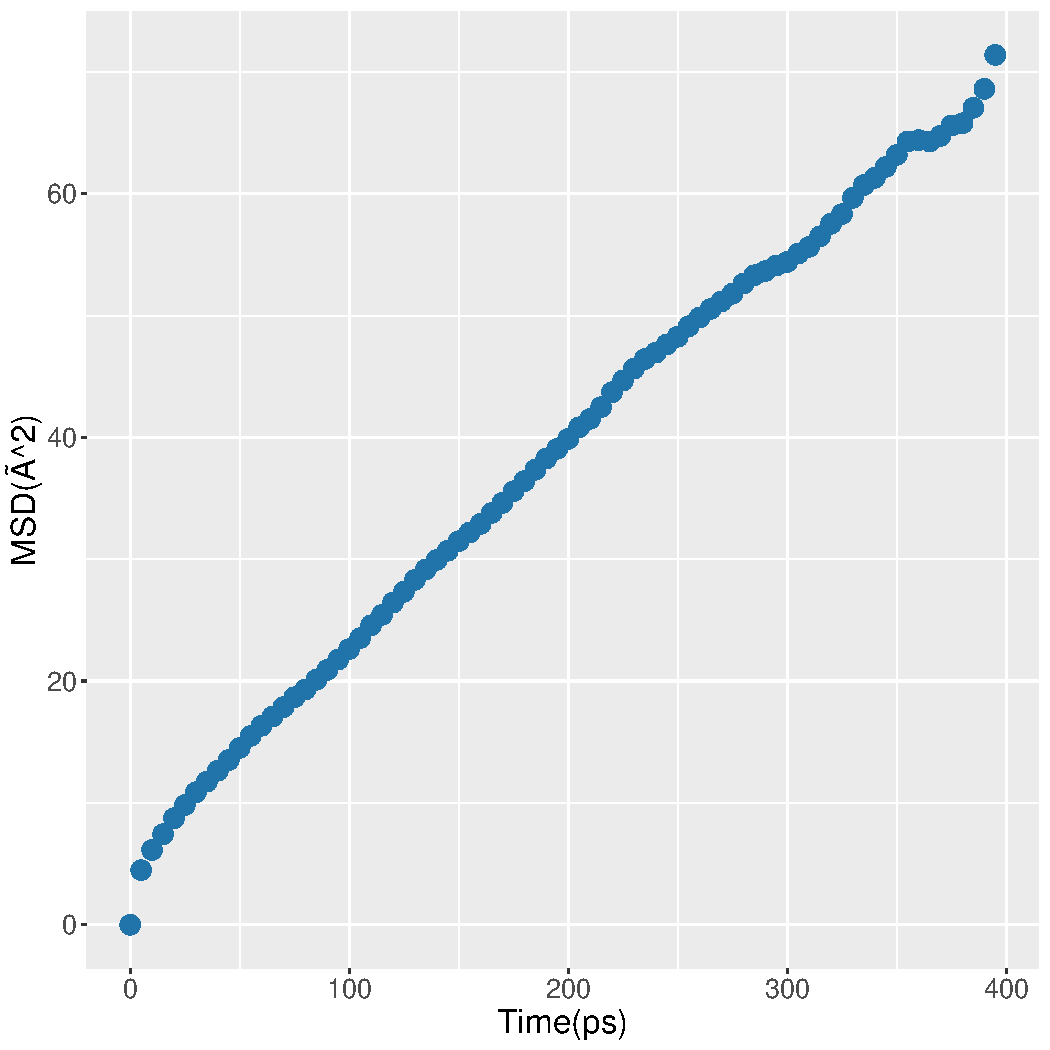
\includegraphics[width=0.5\textwidth]{figure/MSD.pdf}
    \caption{LJ粒子系统的均方位移图}
    \label{fig:MSD}
\end{figure}
\par{根据斯托克斯 - 爱因斯坦方程,有:}
\begin{equation}
    \lim _{t \rightarrow \infty}\left\langle|\vec{r}(t)-\vec{r}(0)|^{2}\right\rangle= 6 D t
\end{equation}
\par{式中:$D$为粒子的扩散系数。}
\par{因此,当计算时间很长时,体系中所有粒子的扩散系数等于均方位移对时间的曲线斜率的六分之一。}
\subsection{国内外研究现状}
\par{本节介绍了目前国内外学者对脂肪酸甲酯在催化裂化和吸附扩散领域的研究成果。讨论在脂肪酸甲酯催化催化裂化工艺中,H-ZSM-5分子筛相较于其他催化剂的优点,确定了催化剂最佳的硅铝比,以及影响吸附扩散性能的因素。}
\subsubsection{脂肪酸甲酯催化裂化工艺研究}
\par{目前许多学者在不同的催化剂上进行了脂肪酸酯的催化裂化反应,所用到的催化剂包括分子筛催化剂和无定型催化剂等。不同的催化剂对脂肪酸酯的催化想产物分布及原料转化率上都有很大的影响。而即使是同一种催化剂,因为催化剂的性质,如孔结构、酸性、择形度,比表面、结晶度等等性质,也都会对反应结果造成很大影响。比如不同的硅铝比会导致催化剂酸性位数量的不同,而催化中间产物会在酸性位上发生二次裂解,从而生成小分子烃类,所以,硅铝比的多少对反应结果的影响尤为重要。本小节主要介绍了催化剂的种类以及硅铝比对脂肪酸甲酯催化裂化的研究。}
\subparagraph{催化剂种类的影响}
\par{Katikaneni\cite{katikaneni_performance_1995}等人研究了在不同温度条件下,不同裂化催化剂上菜籽油的催化转化的产物分布情况。研究结果表明:H-ZSM-5 与其他沸石和非沸石催化剂相比,反应生成的有机液体产品最多,达63 wt\%,而且对芳烃有更高的选择性。Idem\cite{idem_catalytic_1997}等人研究了菜籽油在 H-ZSM-5、硅铝酸盐、二氧化硅、硅氧化铝、γ- 氧化铝、氧化钙和氧化镁催化剂的催化裂化过程。研究结果表明:高择形性的催化剂(如 HZSM-5 和硅铝酸盐催化剂)允许轻微的二次裂化,从而导致低气体产量和高有机液体产品产量。}
\subparagraph{硅铝比的影响}
\par{Dandik\cite{dandik1998catalytic}等人研究了向日葵废油在不同硅铝比的 H-ZSM-5 催化剂上的催化转化。研究结果表明:催化剂中铝的含量越高,反应的转化率越高。Benson\cite{benson2008heterogeneous}等人利用油酸作为不饱和脂肪酸的模型化合物,在H-ZSM-5 催化剂催化下,研究了不饱和脂肪酸催化转化机理。研究结果表明:在高酸性的形状选择催化剂上,可生产多种产品,包括石蜡、烯烃和芳香族化合物。田华\cite{脂肪酸酯的催化裂化研究}在固定床微反应器上进行了脂肪酸酯催化裂化反应的研究。研究结果表明:只要催化剂存在弱酸位,二次裂化反应即可发生;催化剂的酸性越强,二次反应发生的比例越高,生成更多的汽油、液化石油气等小分子;而催化剂上没有酸性位时,二次反应发生较少,液体产物中存在大量的含氧衍生物。Twaiq\cite{twaiq2003liquid}等人研究了棕榈油在以铝硅酸盐介孔材料为催化剂的催化裂化作用。研究结果表明:催化剂活性随铝含量的增加而提高,最终达到最佳水平,而较高的铝含量降低了棕榈油的结晶度,从而降低了棕榈油的催化裂化活性。}
\subparagraph{总结}
\par{ZSM-5 催化剂相比于其他催化剂,因其特有的孔道结构和表面酸性,提高了汽油等产品的收率;H-ZSM-5 催化剂硅铝比越大,酸性越强,二次反应发生的比例越高,就可以生产更多的汽油,减少了含氧衍生物的生成;但铝含量过高,会导致分子筛的热稳定性下降,孔道直径减小;所以适当硅铝比的 H-ZSM-5 分子筛更适合做脂肪酸甲酯催化裂化的催化剂。本文所采用的硅铝比来自Danu\cite{danuthai2009conversion}等人对辛酸甲酯在H-ZSM-5分子筛上的催化裂化实验。}
\subsubsection{脂肪酸甲酯吸附研究}
\par{分子筛的酸性位点不仅是二次催化发生的地方,也是吸附的主要场所之一,而硅铝比的大小会决定分子筛酸性位的数量。如果分子筛孔径过大,虽然吸附分子可以进入分子筛内表面,但这将导致吸附位数量减少,从而影响饱和吸附量,并且孔径大小对吸附能大小也有影响。脂肪酸甲酯催化裂化的原料中既有饱和酯,也有不饱和酯,既有长链,也有短链,所以研究吸附分子的不饱和度和链长因素对吸附的影响对催化剂的设计尤为重要。}
\subparagraph{硅铝比的影响}
\par{洪新\cite{不同硅铝比ZSM-5的合成及其吸附脱除柴油中苯胺和吡啶的性能}等人研究了不同硅铝比的ZSM-5分子筛对柴油中苯胺和吡啶的吸附脱除性能。研究结果表明:硅铝比较小的ZSM-5的吸附脱除苯胺或吡啶的效果明显优于其他样品。}
\subparagraph{孔径大小的影响}
\par{Zhao\cite{zhao2008investigation}等人采用高精度智能重量分析仪,研究了介孔 ZSM-5 结构的扩散和吸附行为。研究结果表明:与在微孔 ZSM-5 相比,引入的介孔降低了4.6倍扩散 - 吸附活化能;因此,尽管在介孔 ZSM-5 催化剂上B酸位降低,但与微孔 ZSM-5 催化剂相比,轻烯烃总收率提高了 2.47 wt\%。Liu\cite{liu2012adsorption}等人采用高精度智能重量分析和零长柱法,研究了在介孔 HZSM-5 分子筛中正辛烷的吸附扩散性能。研究结果表明:与常规 HZSM-5相比,正辛烷在 H-ZSM-5 分子筛中的吸附活化能显著降低;在分子筛中引入介孔为反应物和产物提供了较短的扩散路径和较高的扩散速率,从而提高了燃料油的收率,增强了甲醇与汽油反应中对催化剂失活的抵抗力。}
\subparagraph{不饱和度的影响}
\par{丁雪\cite{Fcc干气在zsm-5分子筛中吸附的分子模拟及热力学分析}等人应用巨正则蒙特卡罗方法(GCMC) 研究了干气中的主要组分在 ZSM-5 分子筛中的吸附行为。研究结果表明:与其它组分相比,乙烯在 ZSM-5 中的吸附量最大。罗演强\cite{生物柴油组分的润滑性能及其在铁表面吸附行为模拟探究}采用 Materials Studio 软件模拟不同酯类在铁表面的吸附行为。研究结果表明:不饱和脂肪酸甲酯具有更强极性的分子的单分子吸附能明显提高。}
\subparagraph{碳链长度的影响}
\par{谭雅文\cite{催化裂化干气组分在ZSM-5中的吸附模拟研究}应用巨正则蒙特卡洛方法(GCMC)进行了干气主要组分在 ZSM-5 中的吸附模拟研究。研究结果表明:C1 $\sim$ C6烷烃的吸附热与氢原子数之间存在线性关系, 并且分子体积越大, 吸附能力越强。Meyer\cite{de2003packing}等人采用间歇吸附技术研究了 C5$\sim$C22 直链烷烃在 ZSM-5 上的液相吸附。研究结果表明:烷烃的饱和容量很大程度上取决于链长。吸附的每单位晶胞 -\ch{C H_x} 基团的数量在 C7 和 C8 之间急剧下降,然后稳定上升,达到 C14$\sim$C22的平稳期。王勇利\cite{C2-6烯烃在h-zsm-5分子筛周期性模型上吸附的理论研究}等人采用密度泛函理论研究了 C2$\sim$C6 直链烯烃在 H-ZSM-5 分子筛上的吸附行为。研究结果表明:对于 C2$\sim$C6 直链烯烃,随着碳数的增加,烯烃的吸附能以 - 12 kJ/mol 的常数线性增大;烯烃在分子筛孔道中吸附时,范德华力起主要作用,碳数增加其影响增大。}
\subparagraph{温度和压力的影响}
\par{李健博\cite{几种气体在ZSM-5分子筛上吸附的模拟与实验研究}分别用实验和模拟的方法,研究了小分子气体在ZSM-5分子筛上的吸附。研究结果表明:四种气体在ZSM-5分子筛上的吸附量随温度的升高而减小,随压力的增大而增加,吸附量随压力的变化规律与实验一致。余英哲\cite{氮气、氩气、氧气在ZSM-5分子筛上吸附的分子模拟研究}等人基于 GCMC 原理,采用分子模拟方法研究了三种小分子气体在 ZSM-5 分子筛上的吸附变化规律。研究结果表明:三种气体的吸附等温线在压力较低的范围,曲线斜率较大,吸附量随压力的增大而迅速增加;压力较高的范围,曲线斜率变小,吸附量随压力的增大而缓慢增加,出现吸附饱和现象;吸附量随温度的升高而减小。}
\subparagraph{总结}
\par{硅铝比对分子的影响主要表现硅铝比越低,其酸性位越多,有更多的吸附活性位,吸附性能更好;更大的孔径导致吸附分子对分子筛活性位访问的增强,吸附活化能也显著降低,这是因为介孔分子筛为吸附分子提供了更短的扩散路径和更低的扩散阻力;吸附分子中碳碳双键与吸附位之间形成 π 配位超分子复合物,相互作用更强,使吸附分子的吸附量增大;附量随温度的升高而减小,随压力的增大而增加。}
\subsubsection{脂肪酸甲酯扩散研究}
\par{目前研究结果已经表明,孔径大小对分子筛的择形性有重要影响。而介孔分子筛相较于传统的微孔分子筛,有更大的孔径,对吸附分子空间位阻更小,且扩散路径长度减小,对扩散有促进作用。但是孔径变大,分子筛变面积相应会减小,酸性位数量也减小,对给催化裂化反应带来不利影响。所以有学者提出在微孔分子筛里加入介孔分子筛,从而改善分子筛的传质效果。}
\subparagraph{孔径大小的影响}
\par{Christensen\cite{christensen2003catalytic}等人研究了苯在介孔 H-ZSM-5 分子筛上的催化烷基化反应。结果表明,介孔 H-ZSM-5 分子筛相对于传统的微孔 H-ZSM-5 分子筛,具有着更高效的质量传递性质,在催化活性和选择性上都有了巨大的改善。Meunier\cite{meunier2012influence}等人通过原位漫反射红外傅立叶变换光谱研究邻二甲苯和异辛烷的解吸。研究结果表明:相比于微孔分子筛,在介孔分子筛上的特征扩散路径长度减少了 4 倍;这些结果证实了通过后合成改性引入晶内介孔后,在扩散限制反应中改善了微孔分子筛分子筛的扩散能力。}
\subparagraph{总结}
\par{介孔 H-ZSM-5 分子筛相对于传统的微孔 H-ZSM-5 分子筛,其特征扩散路径长度减少,具有着更高效的质量传递性质,在催化活性和选择性上都有了巨大的改善。}


\subsubsection{总结}
\par{目前,虽然国内外许多研究者\cite{biswas_effect_2014,twaiq2003liquid,katikaneni_performance_1995}已经通过实验测得了大量的脂肪酸甲酯催化裂化的数据,大量学者\cite{2006Investigation,liu2012adsorption,丙烷在不同硅铝比的NanZSM-5型分子筛上的吸附性质的分子模拟,不同硅铝比ZSM-5的合成及其吸附脱除柴油中苯胺和吡啶的性能}也利用实验测定、理论计算和分子模拟的方法对吸附分子在H-ZSM-5分子筛上的吸附和扩散行为进行了研究,但关于脂肪酸甲酯在不同孔径H-ZSM-5分子筛中的吸附扩散研究目前尚缺。所以文本的研究对于了解脂肪酸甲酯在不同孔径H-ZSM-5 分子筛上的吸附和扩散机理以及催化剂的制备具有指导意义。}

\subsection{本课题研究内容}
\par{主要研究内容如下}:
\begin{enumerate}
    \item 文献调研,查出脂肪酸酯芳构化最常用的 ZSM-5 分子筛的硅铝比,计算温度为 623K、673K、723K 和 773K 四个温度,压力范围为 0-500kPa 条件下,脂肪酸甲酯的吸附等温线、等量吸附能和吸附位,根据吸附等温线拟合出饱和吸附量和吸附平衡常数。研究并解释了温度、压力、孔径、不饱和度和链长对等量吸附能、饱和吸附量和吸附平衡常数的影响。
    \item 确定吸附位,给出低压和高压下的吸附构型图,从而得到丁酸甲酯在分子筛内的吸附情况(在孔道内的分布)。并考察不同类型的不饱和脂肪酸酯在分子筛内的吸附位,比较不饱和脂肪酸酯和饱和脂肪酸酯吸附位的不同之处。
    \item 比较丁酸甲酯在微孔、20Å 和 60Å 内的吸附扩散情况,计算扩散系数,说明了介孔相比微孔的优势所在。
\end{enumerate}

	%建模
	\section{模型构建与结构优化}
\par{本章通过 Materials Studio 8.0 中的Materials Visualizer模块来构建丁酸甲酯、丁烯酸甲酯、油酸甲酯、反油酸甲酯、正己烷等吸附分子和H-ZSM-5微介孔分子筛的模型。使用 Dmol3模块,采用量子力学的方法优化丁酸甲酯、丁烯酸甲酯、油酸甲酯、反油酸甲酯和正己烷等吸附分子模型结构并对其赋予ESP电荷。使用Forcite模块,采用分子力学的方法优化构建的微介孔H-ZSM-5分子筛模型,并将结构优化后的H-ZSM-5分子筛的XRD与标准谱图进行对比,验证模型的正确性。}
\subsection{吸附分子模型构建与优化}
\subsubsection{Dmol3参数设置}\label{Dmol3参数设置}
\par{本小节使用Dmol3模块对吸附分子进行结构优化以及确定原子ESP电荷,相关参数设置如下:}
\begin{enumerate}
    \item 任务选择:结构优化(Geometry Optimization),精度为Fine精度;
    \item 密度泛函(Functional)选择:广义梯度近似(mGGA-M06L),收敛判据选择Fine精度。能量、梯度和位移的收敛阈值分别为1.0×$10^{-5}$Ha、0.002Ha/Å和0.005Å,采用DIIS技术加速SCF收敛;
    \item 核处理(Core Treatment)选择:考虑所有电子(All Electron),数值基组选择默认的DNP,轨道截断精度为Fine精度;
    \item 性能选择:布局分析(Population analysis)。
\end{enumerate}
\par{与B3LYP泛函相比,mGGA-M06L是目前理论计算中使用的最新和最广的泛函,可以很好地描述弱相互作用,计算结果精度很高\cite{zhao2006new,zhao2011applications}。采用Dmol3 Analysis 的布局分析功能,对结构优化后的分子模型赋予ESP电荷。}
\subsubsection{吸附分子几何优化构象}
\par{使用Materials Visualizer模块搭建吸附分子模型,然后使用Dmol3模块,采用 \ref{Dmol3参数设置} 所设参数对吸附分子进行结构优化并赋予ESP电荷。赋予ESP电荷后的吸附分子的结构优化构象见\reffig{fig:build}。}

\begin{figure}[H]
    \centering

    \subfigure[丁酸甲酯(1.732Å×7.794Å×2.755 Å)]{
    \begin{minipage}[t]{0.5\linewidth}
    \centering
    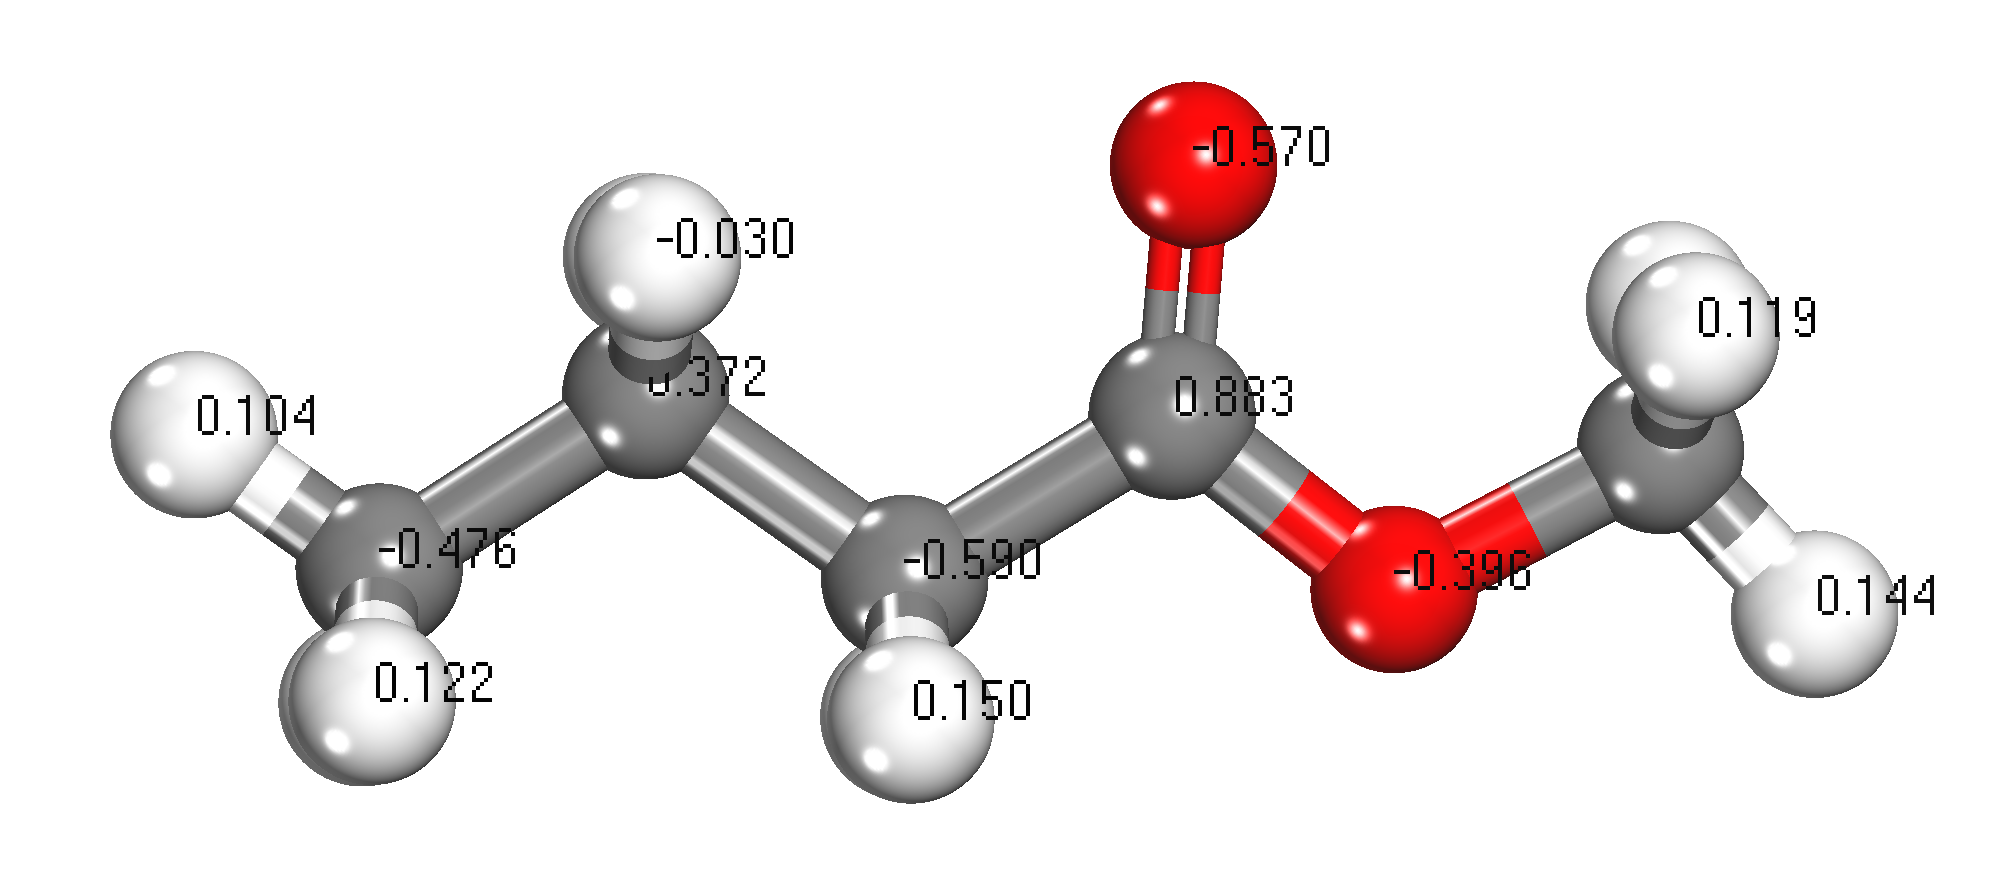
\includegraphics[width=3in]{figure/Building/saturatedC4.png}
    %\caption{fig1}
    \end{minipage}%
    }%
    \subfigure[丁烯酸甲酯(1.732Å×7.757Å×2.755 Å)]{
    \begin{minipage}[t]{0.5\linewidth}
    \centering
    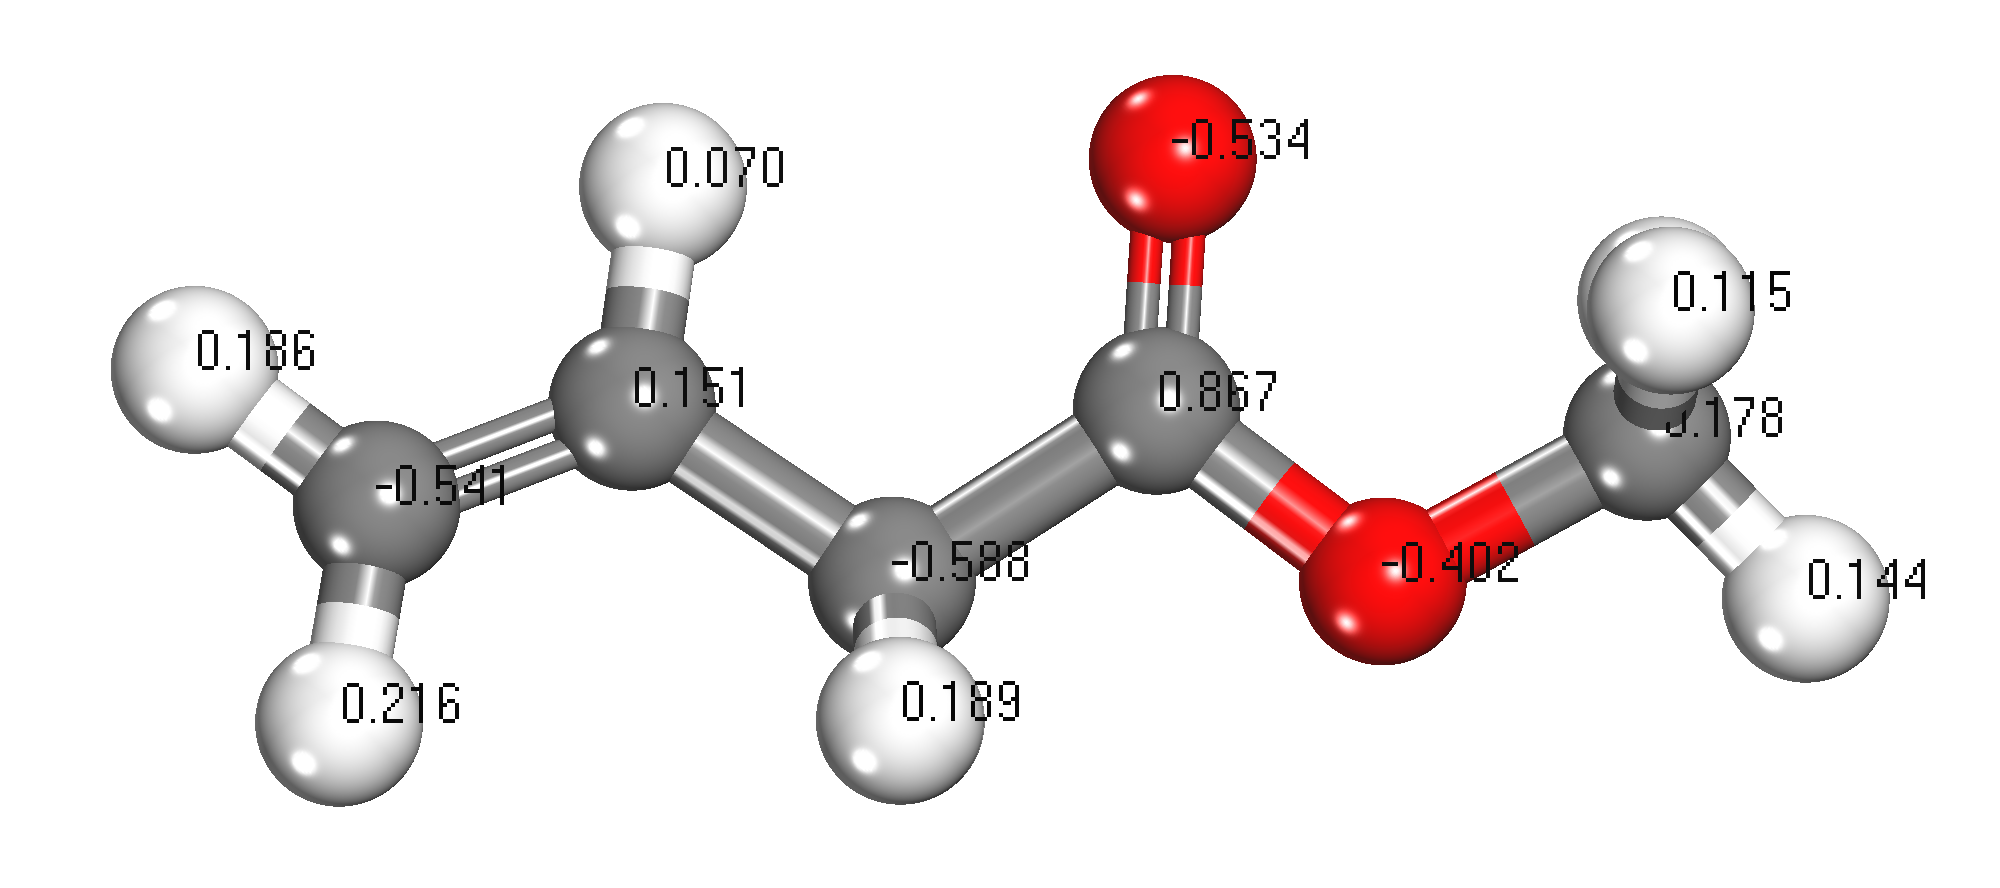
\includegraphics[width=3in]{figure/Building/unsaturatedC4.png}
    %\caption{fig2}
    \end{minipage}%
    }%

    \subfigure[油酸甲酯(2.879Å×25.220Å×2.967 Å)]{
    \begin{minipage}[c]{1\textwidth}
    \centering
    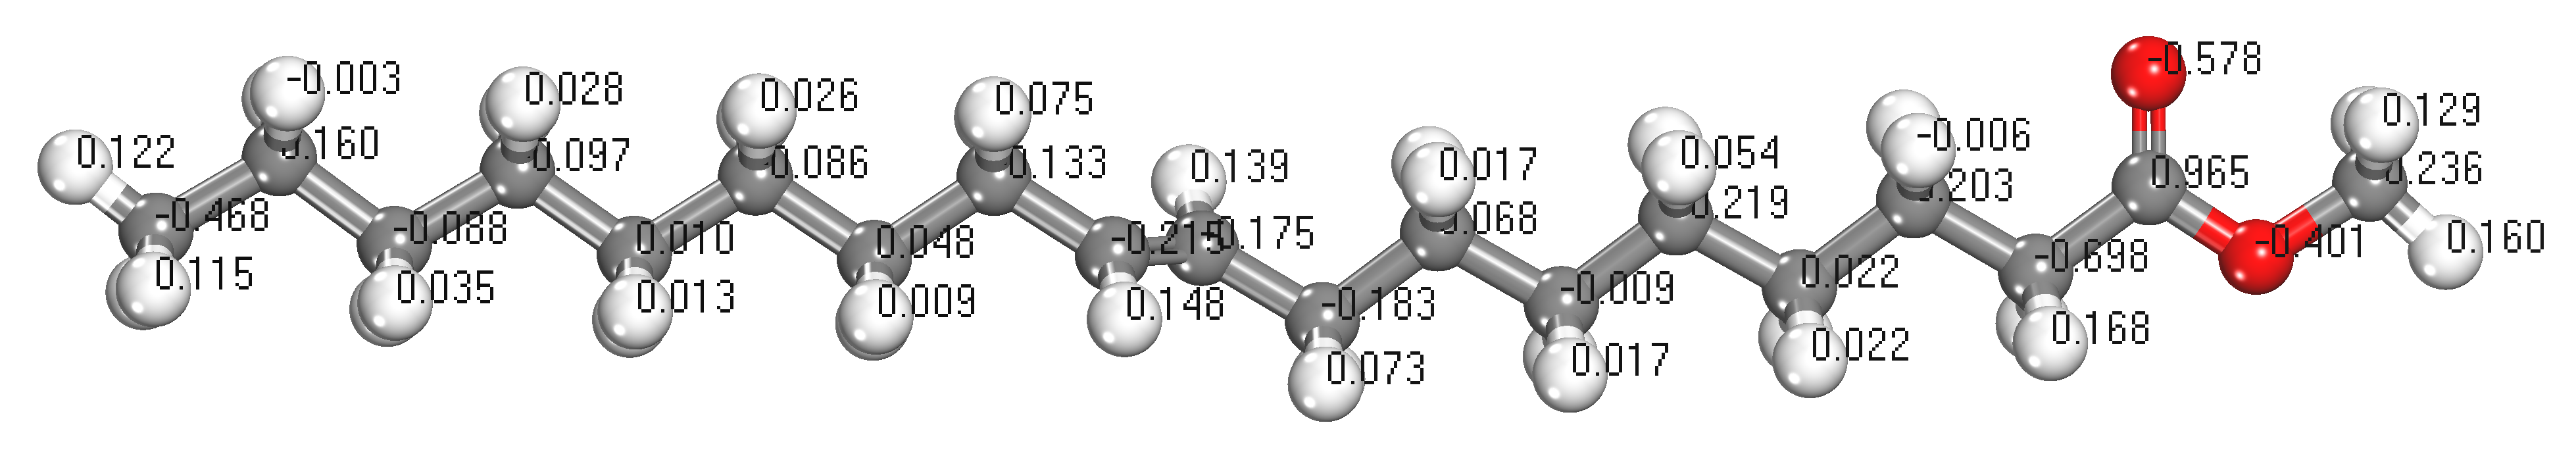
\includegraphics[width=6in]{figure/Building/C18-cis.png}
    %\caption{fig2}
    \end{minipage}%
    }%

    \subfigure[反油酸甲酯(2.879Å×24.579Å×3.017Å)]{
    \begin{minipage}[c]{1\textwidth}
    \centering
    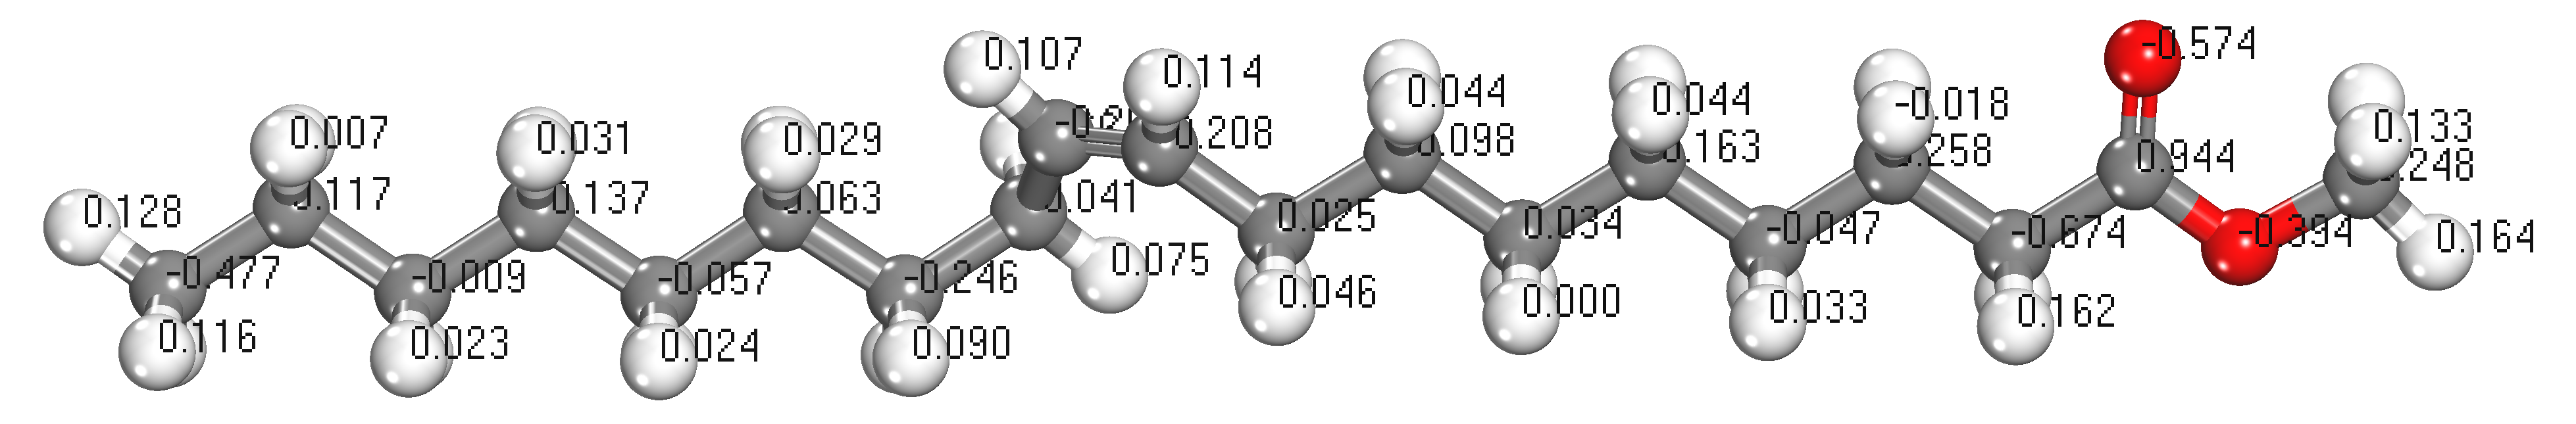
\includegraphics[width=6in]{figure/Building/C18-trans.png}
    %\caption{fig2}
    \end{minipage}%
    }%

    \subfigure[正己烷(1.732Å×8.141Å×2.511 Å)]{
    \begin{minipage}[t]{0.5\linewidth}
    \centering
    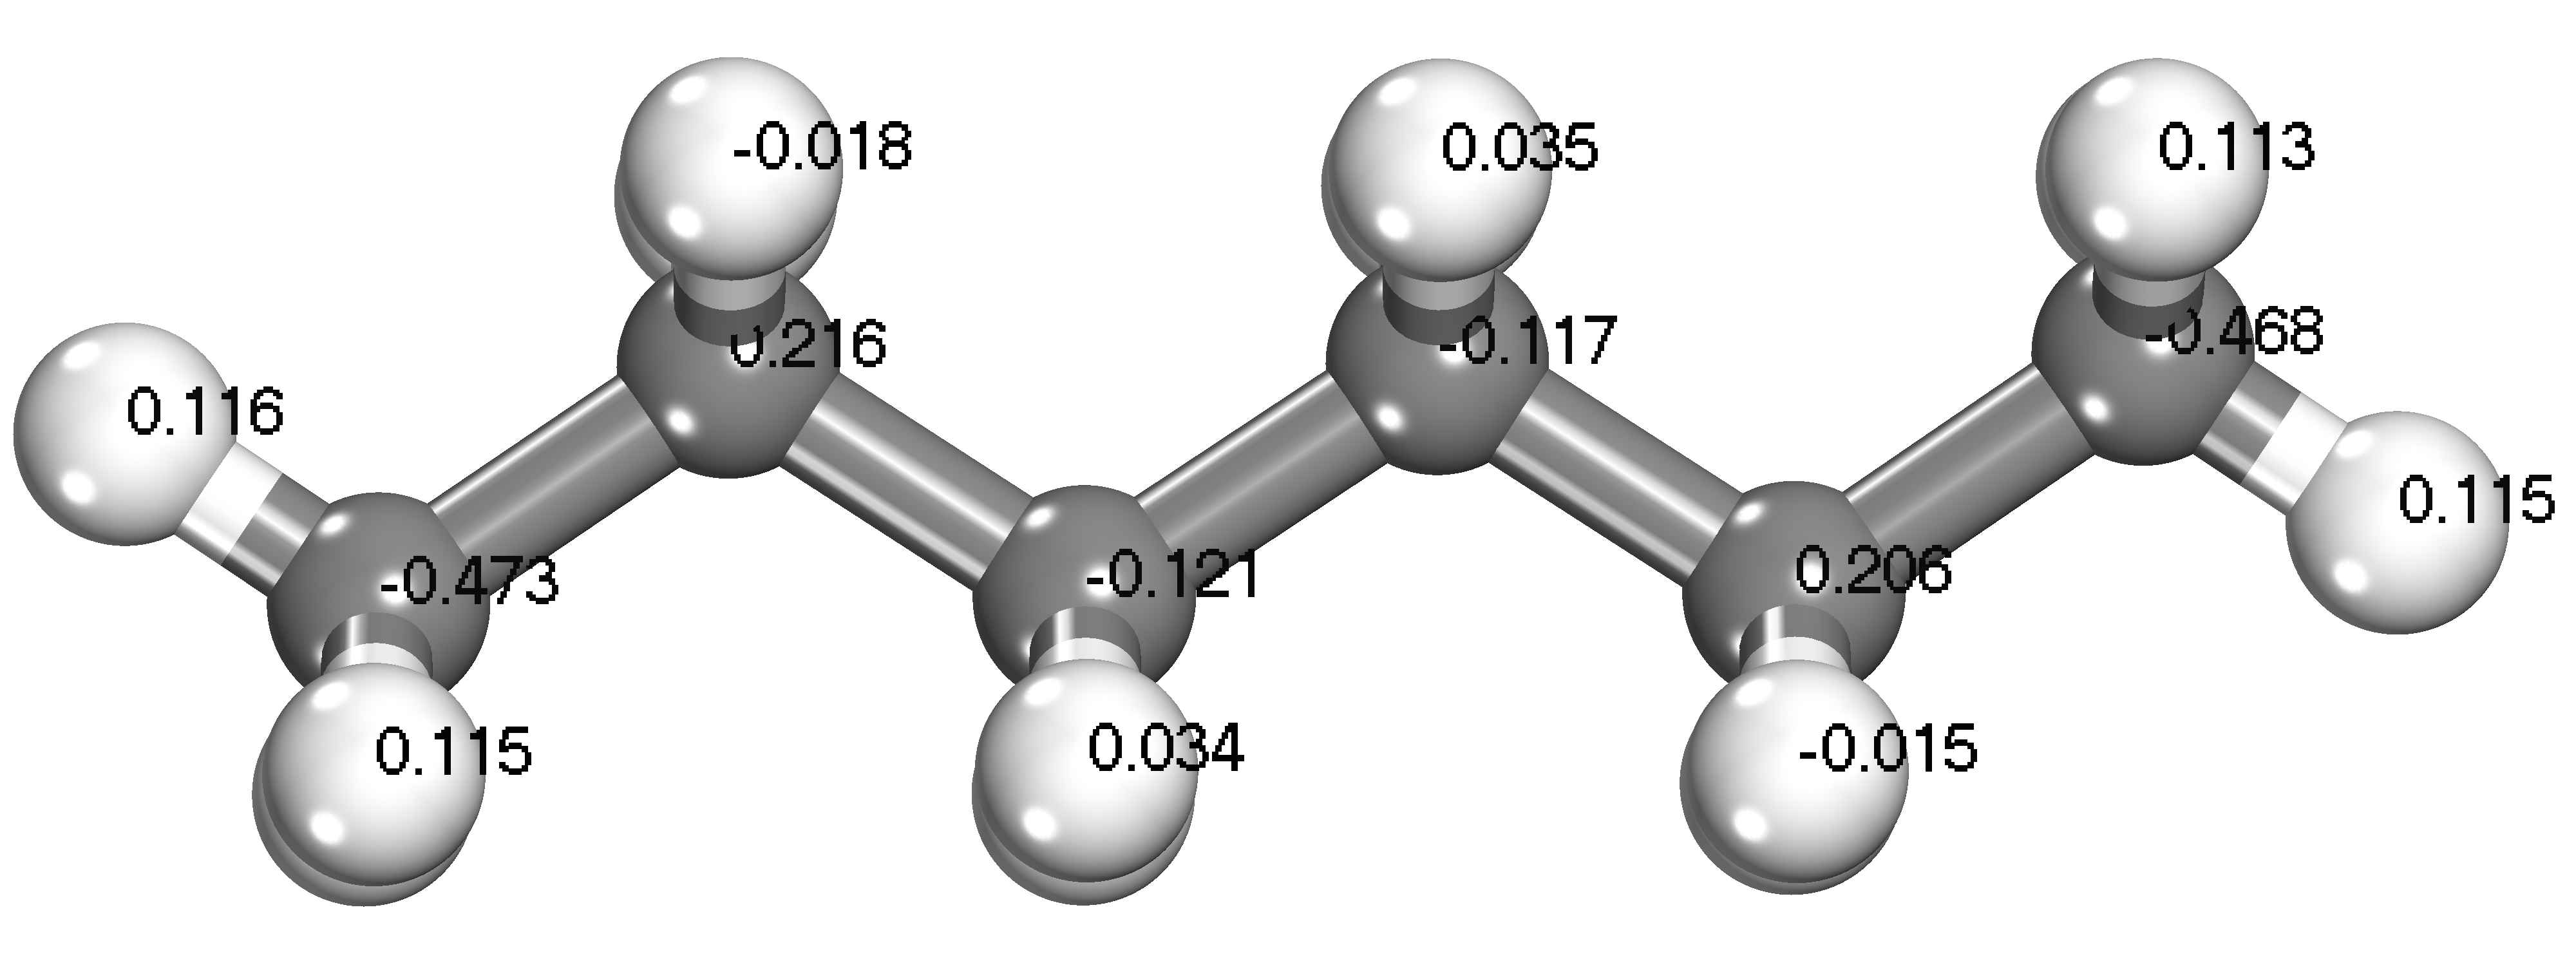
\includegraphics[width=3in]{figure/Building/C6.png}
    %\caption{fig2}
    \end{minipage}%
    }%
    \caption{吸附分子几何优化构象和ESP电荷图}
    \label{fig:build}
\end{figure}

% \subsubsection{丁酸甲酯模型结构}
% \par{本文通过使用Materialss Studio 8.0中Materialss Visualizer模块搭建丁酸甲酯模型,然后使用Dmol3模块对其设置上述参数,然藏对丁酸甲酯模型进行结构优化。优化后的丁酸甲酯分子模型的三维尺寸为1.732Å×7.794Å×2.755 Å,其具体三维结构见\reffig{fig:sC4ESP}。H-ZSM-5分子筛的正弦孔道孔径为5.5Å×5.1Å,直孔道孔径为5.3Å×5.6Å\cite{baerlocher2007atlas},故丁酸甲酯分子可以通过H-ZSM-5分子筛的孔道。将优化后的丁酸甲酯模型用Dmol3 Analysis赋予ESP电荷,其电荷分布见\reffig{fig:sC4ESP},其中C原子为灰色,H原子为白色,O原子为红色。}
% \begin{figure}[H]
%     \centering
%     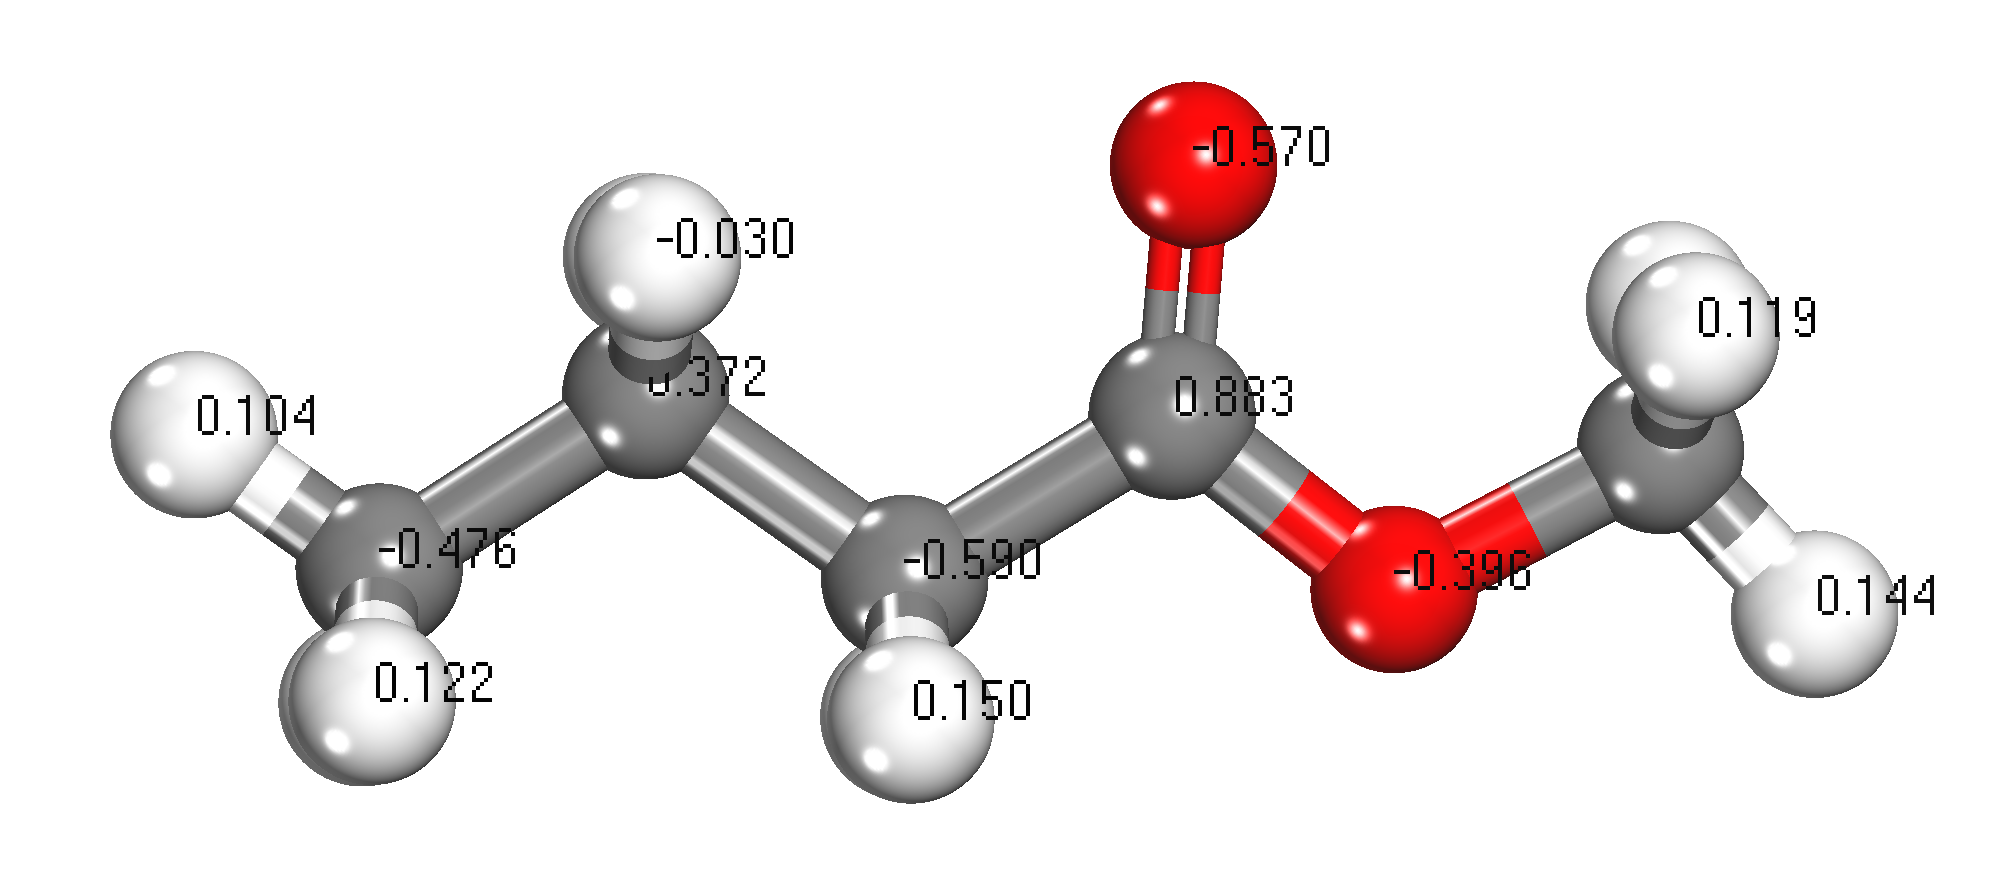
\includegraphics[width=0.6\textwidth]{figure/Building/saturatedC4.png}
%     \caption{丁酸甲酯模型电荷分布图}
%     \label{fig:sC4ESP}
% \end{figure}
% \subsubsection{丁烯酸甲酯模型结构}
% \par{优化后的丁酸甲酯分子模型的三维尺寸为1.732Å×7.757Å×2.755 Å,其具体三维结构见\reffig{fig:uC4ESP}。}
% \begin{figure}[H]
%     \centering
%     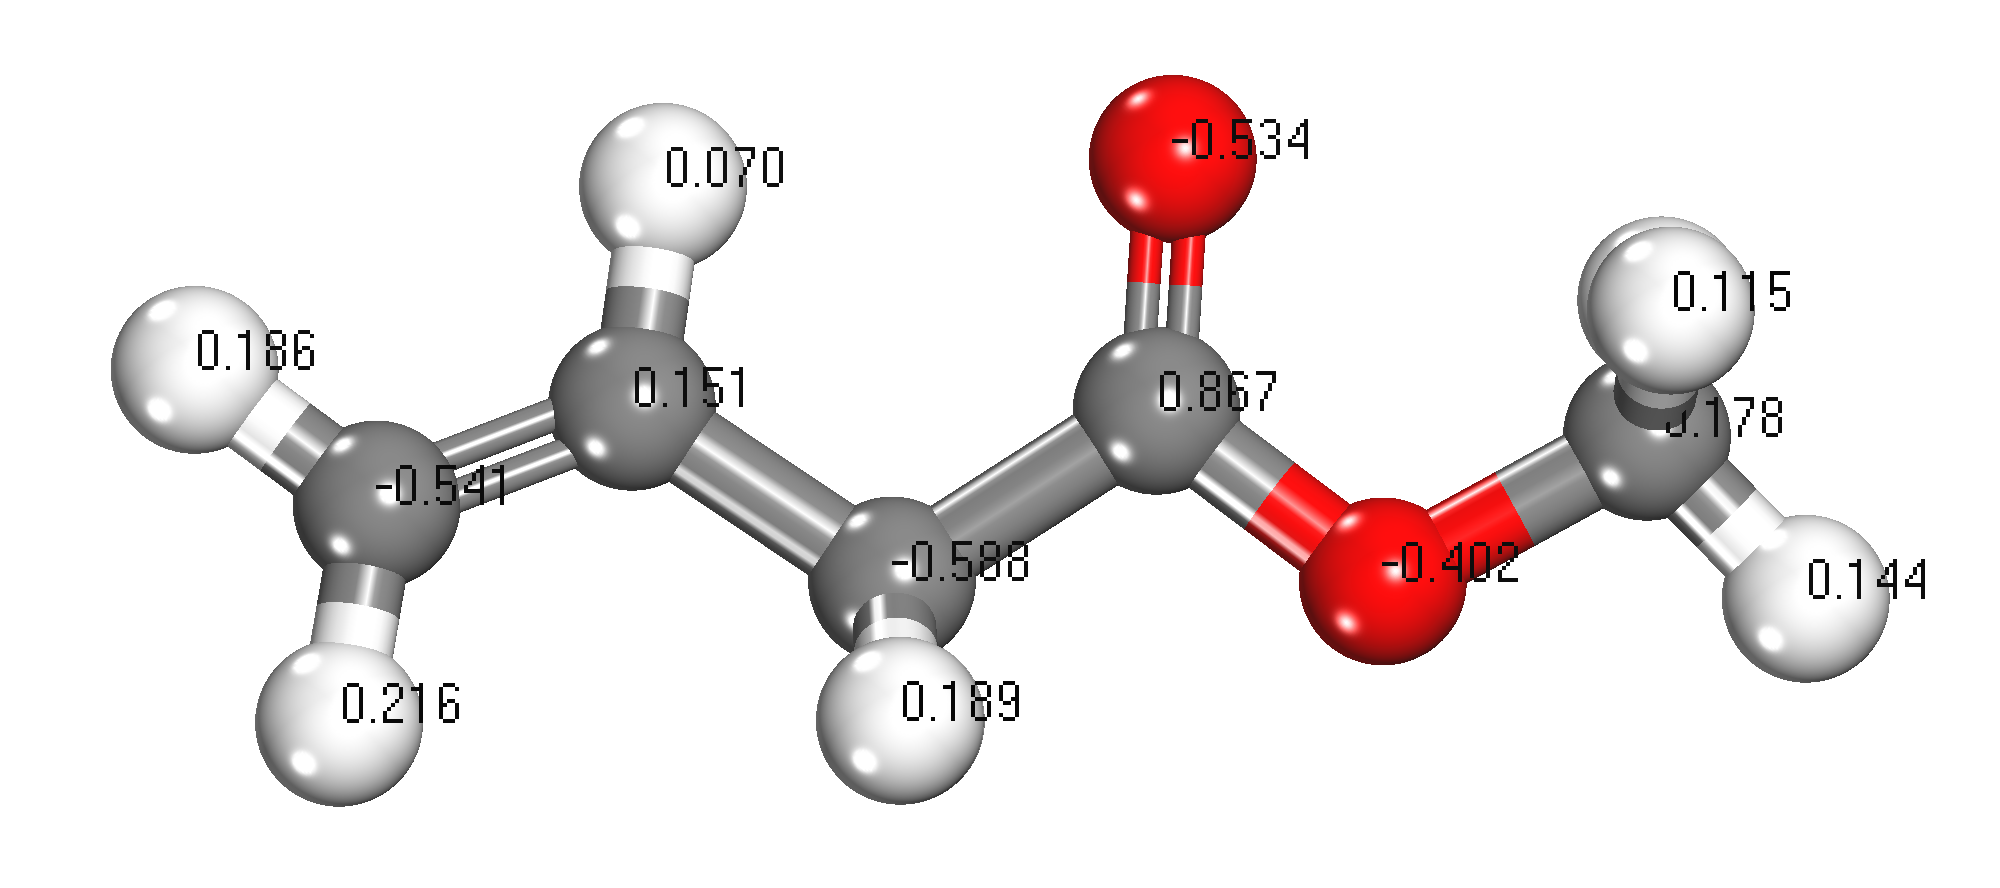
\includegraphics[width=0.6\textwidth]{figure/Building/unsaturatedC4.png}
%     \caption{丁烯酸甲酯模型电荷分布图}
%     \label{fig:uC4ESP}
% \end{figure}
% \subsubsection{乙酸甲酯模型结构}
% \par{优化后的乙酸甲酯分子模型的三维尺寸为1.732Å×5.228Å×2.755 Å,其具体三维结构见\reffig{fig:C2ESP}。}
% \begin{figure}[H]
%     \centering
%     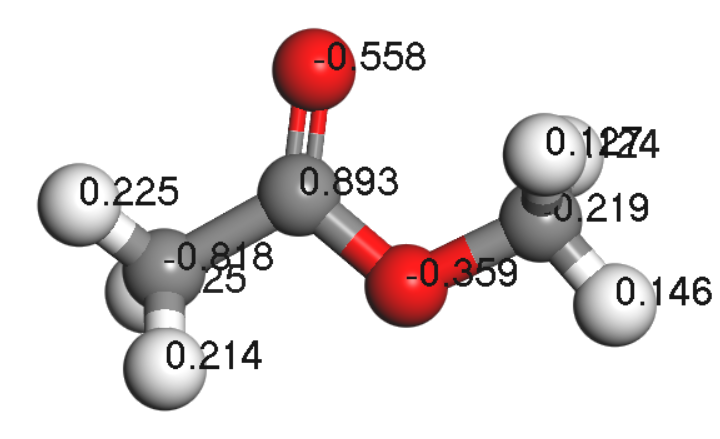
\includegraphics[width=0.5\textwidth]{figure/Building/C2.png}
%     \caption{乙酸甲酯模型电荷分布图}
%     \label{fig:C2ESP}
% \end{figure}
% \subsubsection{丙酸甲酯模型结构}
% \par{优化后的丙酸甲酯分子模型的三维尺寸为1.732Å×6.504Å×2.755 Å,其具体三维结构见\reffig{fig:C3ESP}。}
% \begin{figure}[H]
%     \centering
%     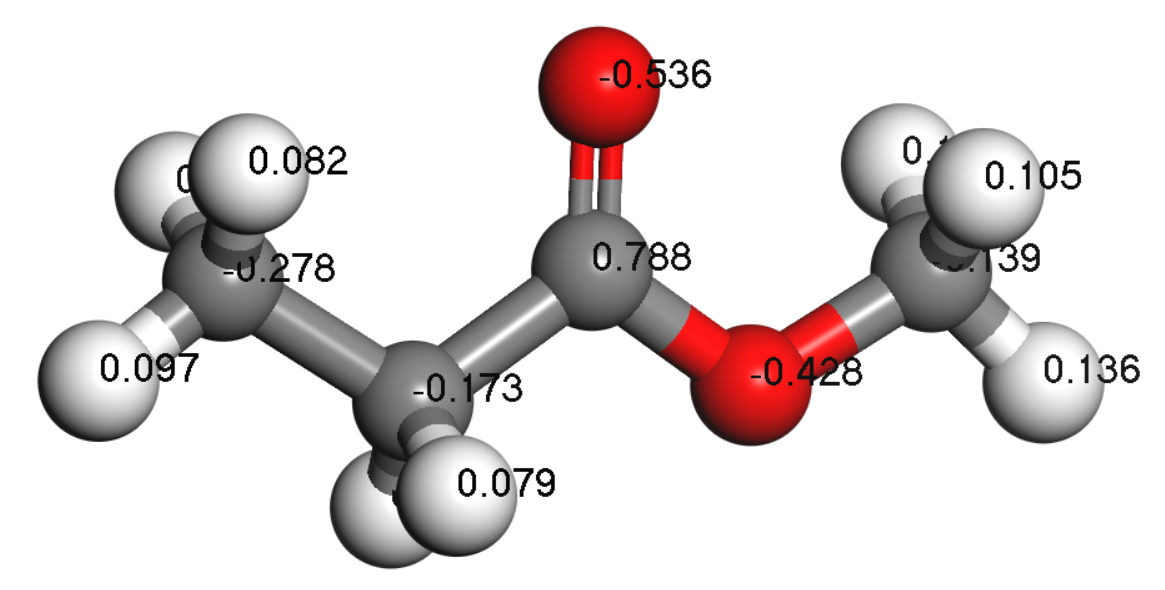
\includegraphics[width=0.6\textwidth]{figure/Building/C3.png}
%     \caption{丙酸甲酯模型电荷分布图}
%     \label{fig:C3ESP}
% \end{figure}
% \subsubsection{戊酸甲酯模型结构}
% \par{优化后的戊酸甲酯分子模型的三维尺寸为1.732Å×9.035Å×2.755 Å,其具体三维结构见\reffig{fig:C5ESP}。}
% \begin{figure}[H]
%     \centering
%     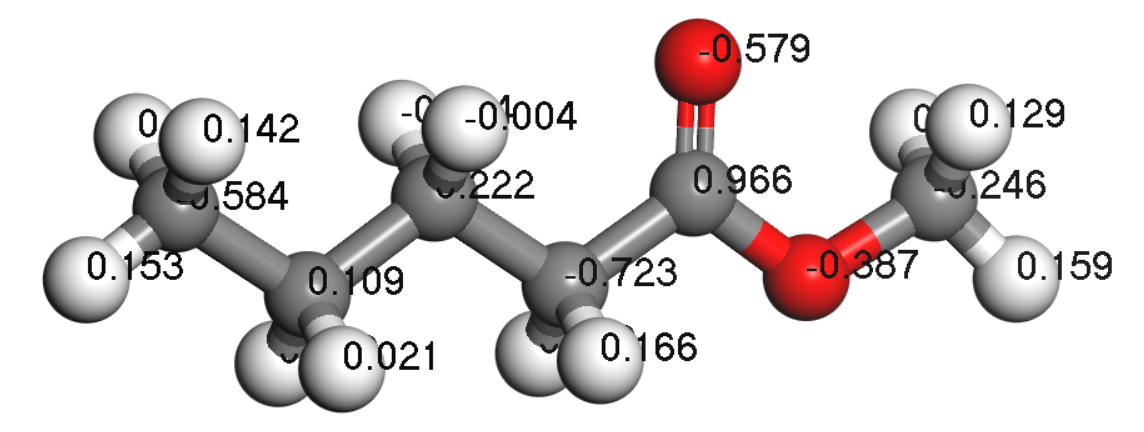
\includegraphics[width=0.6\textwidth]{figure/Building/C5.png}
%     \caption{戊酸甲酯模型电荷分布图}
%     \label{fig:C5ESP}
% \end{figure}
% \subsubsection{正己烷模型结构}
% \par{优化后的正己烷分子模型的三维尺寸为1.732Å×8.141Å×2.511 Å,其具体三维结构见\reffig{fig:C6ESP}。}
% \begin{figure}[H]
%     \centering
%     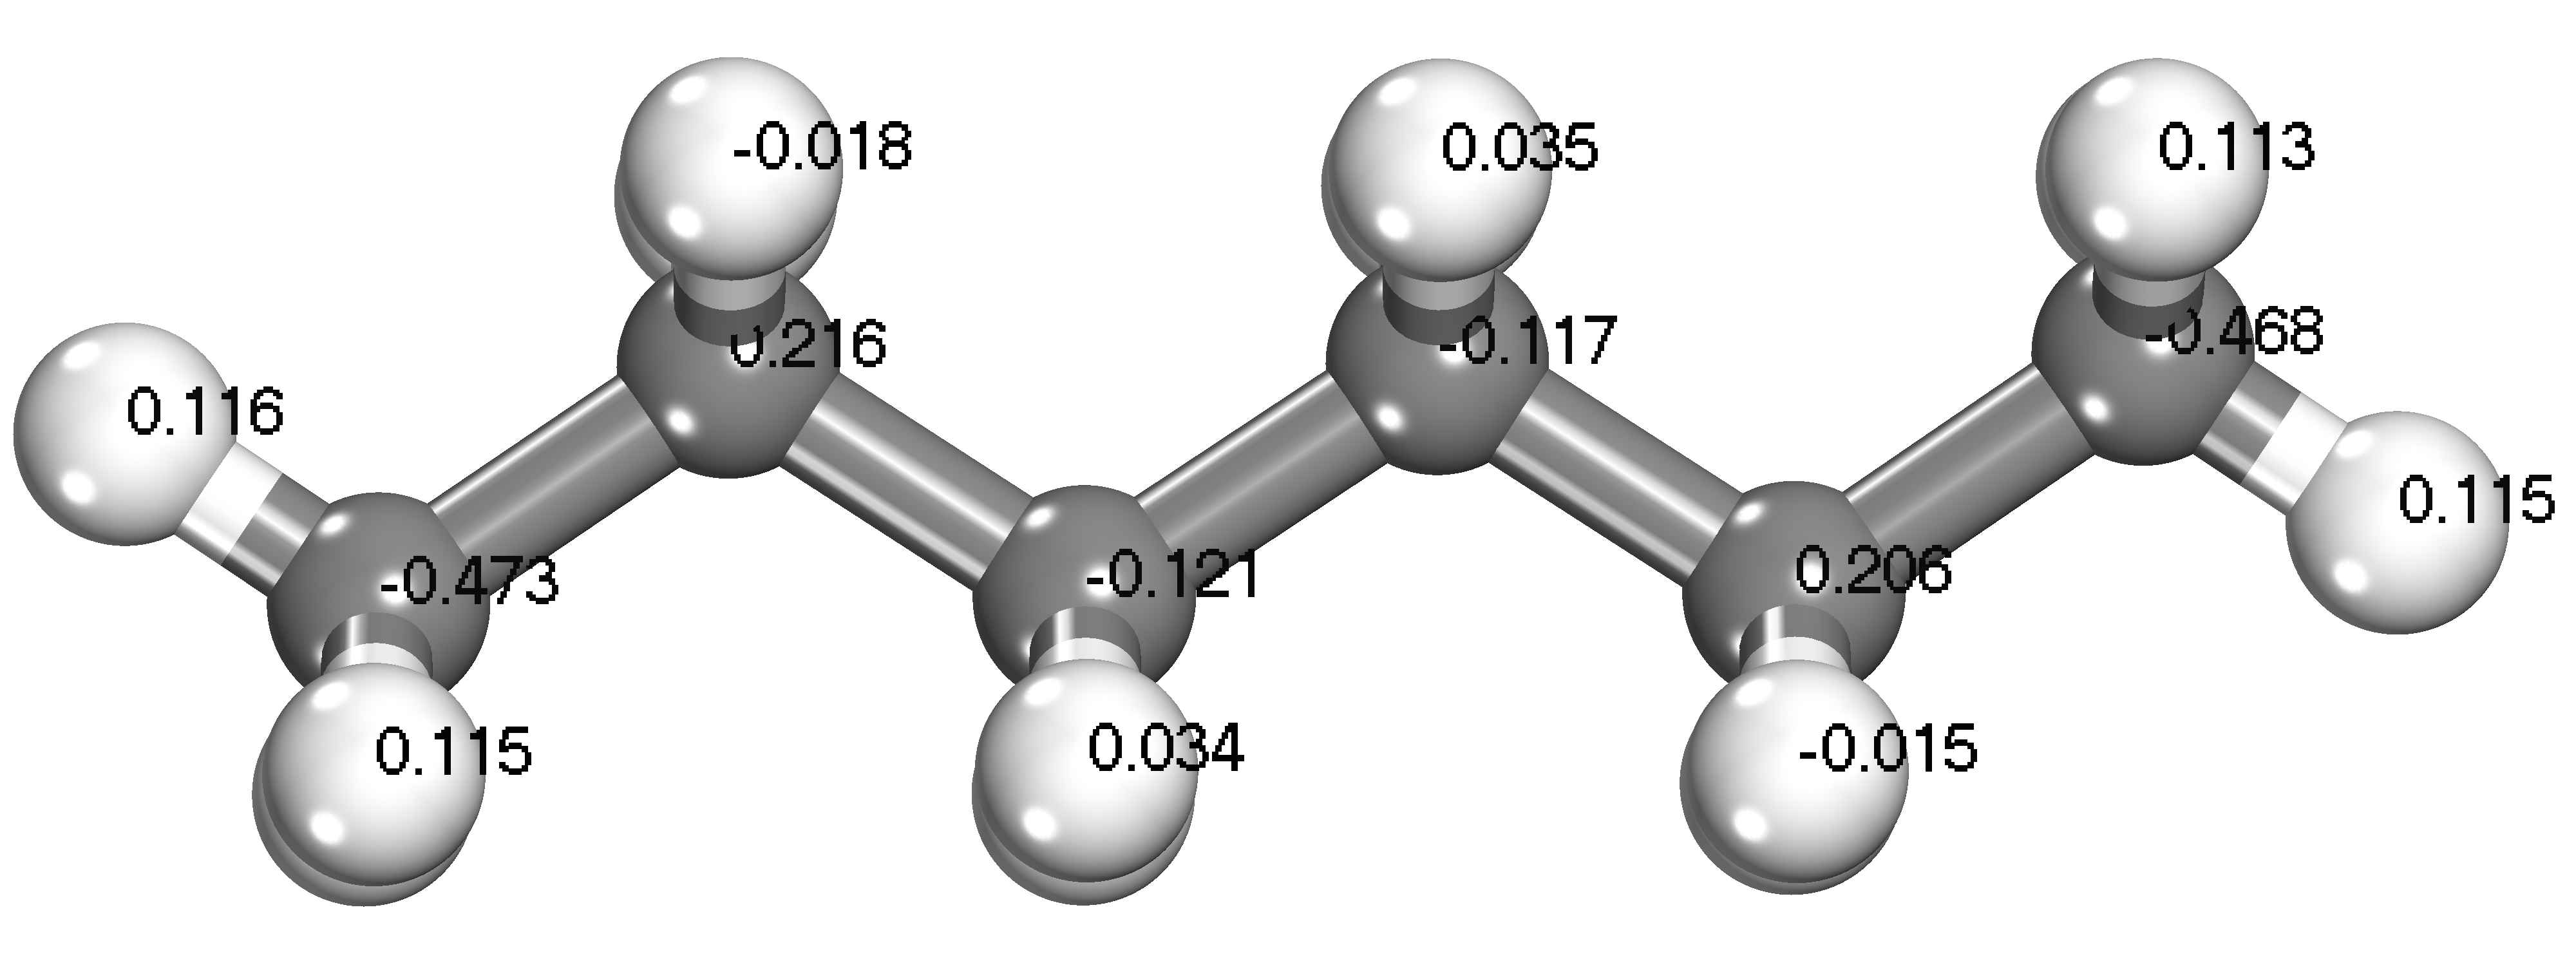
\includegraphics[width=0.6\textwidth]{figure/Building/C6.png}
%     \caption{正己烷模型电荷分布图}
%     \label{fig:C6ESP}
% \end{figure}
\subsection{H-ZSM-5微介孔分子筛模型构建与优化}
\subsubsection{Forcite 参数设置}\label{Forcite 参数设置}
\par{本节使用Forcite模块对H-ZSM-5分子筛进行结构优化以及确定各原子的电荷,相关参数设置如下:}
\begin{enumerate}
    \item 任务选择:结构优化(Geometry Optimization),收敛精度选择Ultra-Fine精度,算法选择默认的Smart方法;
    \item 力场(Forcefield)采用COMPASS\uppercase\expandafter{\romannumeral2}力场,其适用于大多数有机物、无机物、金属及其氧化物与卤化物,电荷选择Forcefield  assigned;
    \item 能量计算精度选择: Ultra-Fine精度;
    \item 加和方法(Summation method)中的静电相互作用(Electrostatic)选择埃瓦德方法(Ewald \& Group),非键相互作用(van der Waals)选择基于原子(Atom based)。
\end{enumerate}
% \par{一个合适的力场不仅能够计算出分子合理的最低构象,也能够准确地描述分子筛和吸附质分子之间的相互作用,所以力场选取的正确与否很大程度上决定了模拟结果是否可靠。本文选取的力场为COMPASS\uppercase\expandafter{\romannumeral2}。COMPASS\uppercase\expandafter{\romannumeral2}力场将 COMPASS 力场的应用范围扩大,可以用来预测聚合物和药物,并且修正了COMPASS力场的参数,使结果更加可靠\cite{Sun2016COMPASS}。而为了验证 COMPASS 力场的有效性,孙淮及其他研究者曾经对单个分子、液态分子及晶体分子共 28 类分子进行模拟验证\cite{分子模拟与高分子材料},发现COMPASS 力场能够模拟小分子与高分子,一些金属离子、金属氧化物与金属。}
\subsubsection{微孔模型构建及其优化}
\par{先导入MFI分子筛模型,其空间群为Pnma正交晶系结构。模拟采用2×2×3个晶胞\cite{bu2018diffusion},晶胞参数:a=40.044Å,b=39.798Å,c=40.149Å,α=β=γ=90°。首先根据文献\cite{danuthai2009conversion}的实验表征结果,将分子筛的硅铝比改为36,并根据文献\cite{zheng2014influence,zheng2016molecular}在Al原子相邻的O原子上引入H原子平衡电荷并作为反应活性位,并且H原子指向分子筛晶体中原有的骨架原子。最后使用Forcite模块进行结构优化和电荷赋值。}
\par{微孔H-ZSM-5分子筛超胞的分子式为:\ch{H_{31}O_{2304}Al_{31}Si_{1121}},有31个活性位,晶胞参数:a=40.044Å,b=39.798Å,c=40.149Å,α=β=γ=90°。其几何优化结构见\reffig{fig:mZSM},其中Si原子为黄色,Al原子为紫色,O原子为红色,H原子为白色。}
\begin{figure}[H]
    \centering

    \subfigure[A方向]{
    \begin{minipage}[t]{0.25\linewidth}
    \centering
    \includegraphics[width=1.5in]{figure/Building/microporeA.png}
    %\caption{fig1}
    \end{minipage}%
    }%
    \subfigure[B方向]{
    \begin{minipage}[t]{0.25\linewidth}
    \centering
    \includegraphics[width=1.5in]{figure/Building/microporeB.png}
    %\caption{fig2}
    \end{minipage}%
    }%
    \subfigure[C方向]{
    \begin{minipage}[t]{0.25\linewidth}
    \centering
    \includegraphics[width=1.5in]{figure/Building/microporeC.png}
    %\caption{fig2}
    \end{minipage}%
    }%
    \caption{微孔H-ZSM-5分子筛结构优化图}
    \label{fig:mZSM}
\end{figure}
\par{微孔分子筛经Forcite模块优化后,各原子之间的化学键方向发生了改变,H原子朝向也发生变化。模拟结果表明:微孔H-ZSM-5分子筛优化前体系能量为-78772.04 kcal/mol,优化后能量为-86248.41 kcal/mol;此时的分子筛能量最低,结构最稳定。}
\subsubsection{介孔模型构建及其优化}
\par{微孔H-ZSM-5 分子筛由沿B 方向的直通道和沿A 方向的锯齿形通道组成。在构建介孔模型时,选择沿C 方向的介孔来创建三维通道,以提高传质效率\cite{bu2018diffusion}。通过沿H-ZSM-5(4×4×3 单元)和(2×2×3 单元)两个超胞的C 方向切割,构建了60Å 和20Å 两种不同孔径的介孔H-ZSM-5 分子筛模型。两种介孔H-ZSM-5 分子筛模型的微孔壁厚度均为20Å,因此介孔体积分数分别为0.25和0.56。介孔表面硅原子以羟基封端。}
\par{20Å介孔H-ZSM-5分子筛超胞的分子式为:\ch{H_{171}O_{1800}Al_{27}Si_{837}},有27个活性位,晶胞参数:a=40.044Å,b=39.798Å,c=40.149Å。60Å介孔H-ZSM-5分子筛超胞的分子式为:\ch{H_{495}O_{4248}Al_{63}Si_{1953}},有63个活性位,晶胞参数:a=80.088Å,b=79.596Å,c=40.149Å。因为介孔A和B方向的结构和微孔的一样,所以只展示C方向的结构。介孔C方向的几何优化结构见\reffig{fig:2060ZSM},其中Si原子为黄色,Al原子为紫色,O原子为红色,H原子为白色。}
\begin{figure}[H]
    \centering

    \subfigure[20Å]{
    \begin{minipage}[t]{0.5\linewidth}
    \centering
    \includegraphics[width=3in]{figure/Building/20C.png}
    %\caption{fig1}
    \end{minipage}%
    }%
    \subfigure[60Å]{
    \begin{minipage}[t]{0.5\linewidth}
    \centering
    \includegraphics[width=3in]{figure/Building/60C.png}
    %\caption{fig2}
    \end{minipage}%
    }%
    \caption{介孔H-ZSM-5分子筛C方向结构优化图}
    \label{fig:2060ZSM}
\end{figure}

\subsubsection{分子筛中各原子电荷}
\par{优化后的分子筛中各原子电荷如\reftab{tab:ESP}所示。}

\begin{table}[H]
    \centering
    \caption{分子筛各原子所赋电荷表}
    \begin{tabular}{p{5cm}<{\centering}P{-1.3}}
        \toprule
        原子种类&\multicolumn{1}{p{5cm}<{\centering}}{电荷赋值}\\
        \midrule
        Si&1.400\\
        Al&0.800\\
        O&-0.700\\
        H&0.600\\
		\bottomrule
    \end{tabular}
	\label{tab:ESP}
\end{table}


\subsection{模型验证}
\par{为了验证所搭建的分子筛模型的结构是合理的,本文计算了结构优化后的微孔分子筛模型的X射线衍射图(XRD),并将结果和国际沸石协会(IZA-SC)数据库中的ZSM-5分子筛标准X射线衍射图\cite{baerlocher2007atlas}进行对比,结果如\reffig{fig:XRD}所示。从图中发现两者具有相同的特征峰,说明搭建的H-ZSM-5分子筛模型是合理的。}
\begin{figure}[H]
    \centering
    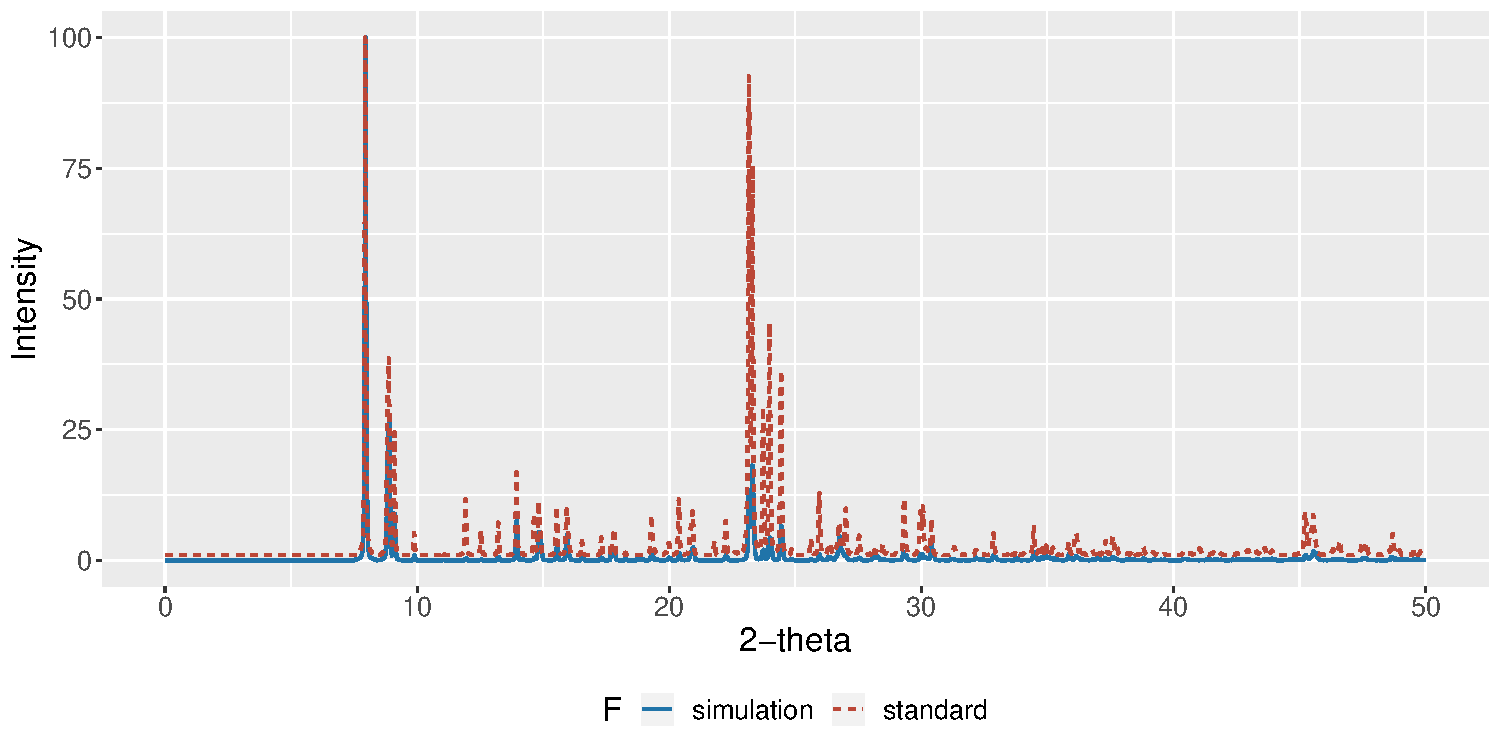
\includegraphics[height=0.5\textwidth]{figure/Building/XRD.pdf}
    \caption{微孔H-ZSM-5分子筛模型XRD与标准谱图对比图}
    \label{fig:XRD}
\end{figure}
\subsection{本章小结}
\par{本章通过Visualizer界面构建了丁酸甲酯、丁烯酸甲酯、油酸甲酯、反油酸甲酯和正己烷分子模型,并用Dmol3模块对进行其结构优化,并计算了ESP电荷,得到了吸附质分子的几何优化构型。}
\par{通过Visualizer界面构建了微介孔H-ZSM-5分子筛模型,并用Forcite模块对其进行结构优化,赋予电荷,得到了吸附剂分子的几何优化构型。}
\par{通过与标准X射线衍射图进行对比,验证了本文所构建的模型是合理的,为下文中吸附分子在H-ZSM-5分子筛中的吸附和扩散的模拟提供了合理的模拟基础。}

	%吸附
	\section{脂肪酸甲酯在H-ZSM-5分子筛上的吸附}
\par{通过传统的实验方法来获得吸附性质的效率很低,尤其是在反应的条件下研究长链分子的吸附更加困难。更重要的是,即使在温和的条件下,对于小分子而言,想通过实验的手段获得吸附位和吸附质构象等信息也是非常困难\cite{van1998chain}。}
\par{所以本章采用上文中构建的模型,使用Sorption模块,进行了丁酸甲酯、丁烯酸甲酯、油酸甲酯和反油酸甲酯在微介孔H-ZSM-5分子筛上的巨正则蒙特卡洛模拟(GCMC),考察了各类吸附分子在H-ZSM-5分子筛上的吸附性能,分析吸附分子链长和不饱和度、分子筛孔径和外界温度压力对于吸附性能的影响。}
\subsection{Sorption 参数设置}\label{Sorption 参数设置}
\par{本节使用Sorption模块进行吸附模拟,相关参数设置如下:}
\begin{enumerate}
    \item 任务选择:固定压力(Fixed pressure);温度设定:623K、673K、723K和773K(催化裂化反应温度);压力范围:0-500kPa内取点;平衡计算步数5000000步,生产步数10000000步;勾选返回最低能量构架(Return lowest energy frames),数量为10。
    \item 计算方法:Metropolis方法;精度选择:Ultra-fine。
    \item 力场选择:COMPASS\uppercase\expandafter{\romannumeral2};电荷选择:Use current。
    \item 加和方法中的静电相互作用选择埃瓦德方法(Ewald \& Group),非键相互作用选择原子基准(Atom based),非键截断值设置为18.5Å(正好小于晶胞最小边长一半)。
\end{enumerate}
\subsection{模型验证}\label{checking}
\par{为了验证本文计算采用的参数的正确性,本文将模拟计算出来的油酸甲酯和反油酸甲酯在微孔H-ZSM-5分子筛中的吸附结果与文献\cite{philippaerts2010selectivity}的实验结果相对比,模拟参数参照上文的参数设置,温度为室温25℃。对比结果如\reftab{tab:C18}所示。}


\begin{table}[H]
    \centering
    \caption{油酸甲酯与反油酸甲酯在H-ZSM-5分子筛内的吸附情况对比表}
    \begin{tabular}{p{2.5cm}<{\centering}p{2.5cm}<{\centering}p{2.5cm}<{\centering}p{2.5cm}<{\centering}p{2.5cm}<{\centering}}
        \toprule
        项目&硅铝比&$K_{ME}$&$K_{MO}$&$\alpha$\\
        \midrule
        实验&40&3.23&3.08&1.05\\
        模拟&36&2.92&2.63&1.02\\
		\bottomrule
    \end{tabular}
	\label{tab:C18}
\end{table}

\par{其中:$K_{ME}$表示反油酸甲酯的平衡吸附常数;$K_{MO}$表示油酸甲酯的平衡吸附常数;$\alpha$表示油酸甲酯与反油酸甲酯饱和吸附量的比值。由\reftab{tab:C18}可知,模拟与实验结果非常接近,误差不超过15\%,所以 \ref{Sorption 参数设置} 的参数设置是合理的。}

\subsection{模拟结果}
\subsubsection{吸附等温线}\label{吸附等温线}
\par{本小节按照 \ref{Sorption 参数设置} 的参数设置,首先计算了模型化合物丁酸甲酯和丁烯酸甲酯在微介孔H-ZSM-5分子筛,0~500kPa的吸附等温线,结果如\reffig{fig:sA}所示。}

\begin{figure}[H]
    \centering

    \subfigure[丁酸甲酯在微孔]{
    \begin{minipage}[t]{0.5\linewidth}
    \centering
    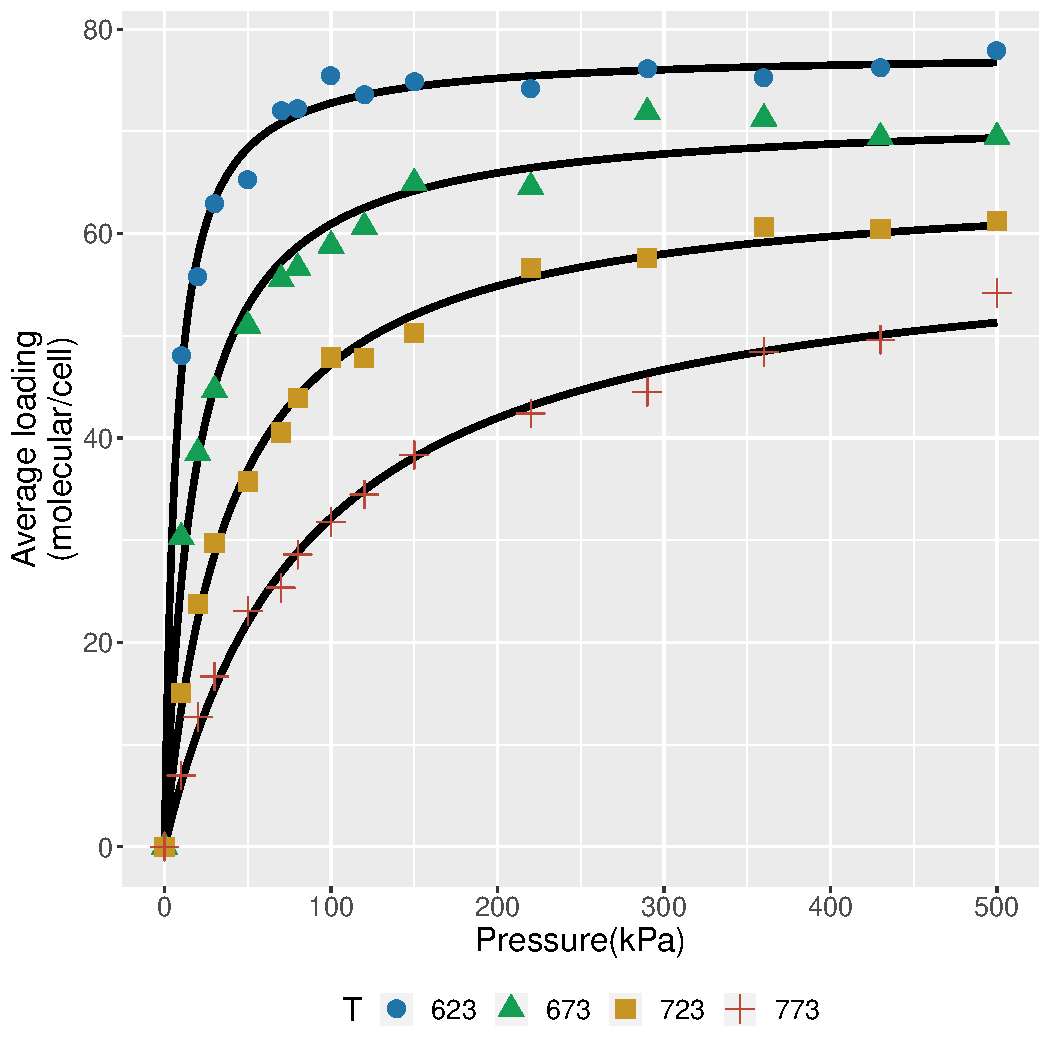
\includegraphics[width=2.7in]{figure/Adsorption/MicroPoreA.pdf}
    %\caption{fig1}
    \end{minipage}%
    }%
    \subfigure[丁烯酸甲酯在微孔]{
    \begin{minipage}[t]{0.5\linewidth}
    \centering
    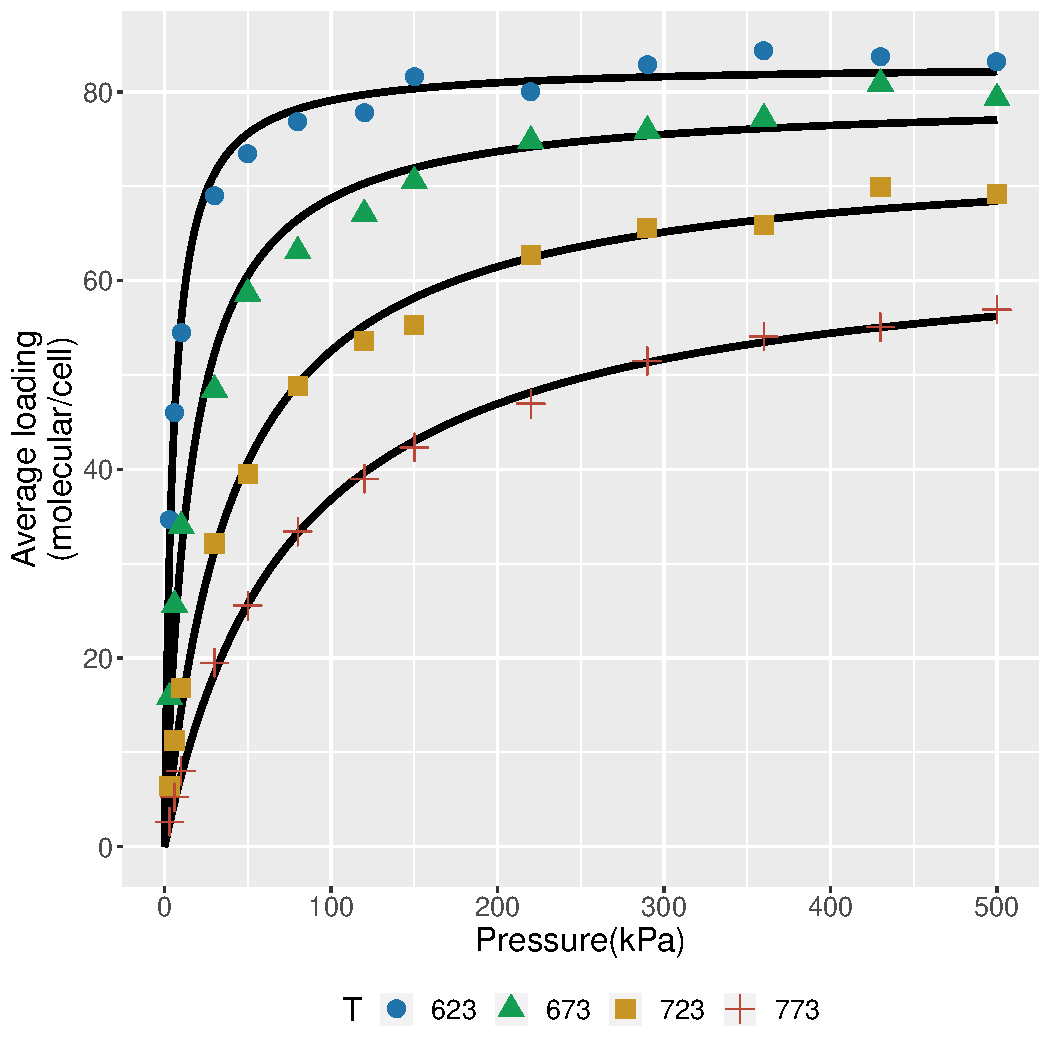
\includegraphics[width=2.7in]{figure/Adsorption/MicroPoreAunsaturated.pdf}
    %\caption{fig2}
    \end{minipage}%
    }%

    \subfigure[丁酸甲酯在20Å介孔]{
    \begin{minipage}[t]{0.5\linewidth}
    \centering
    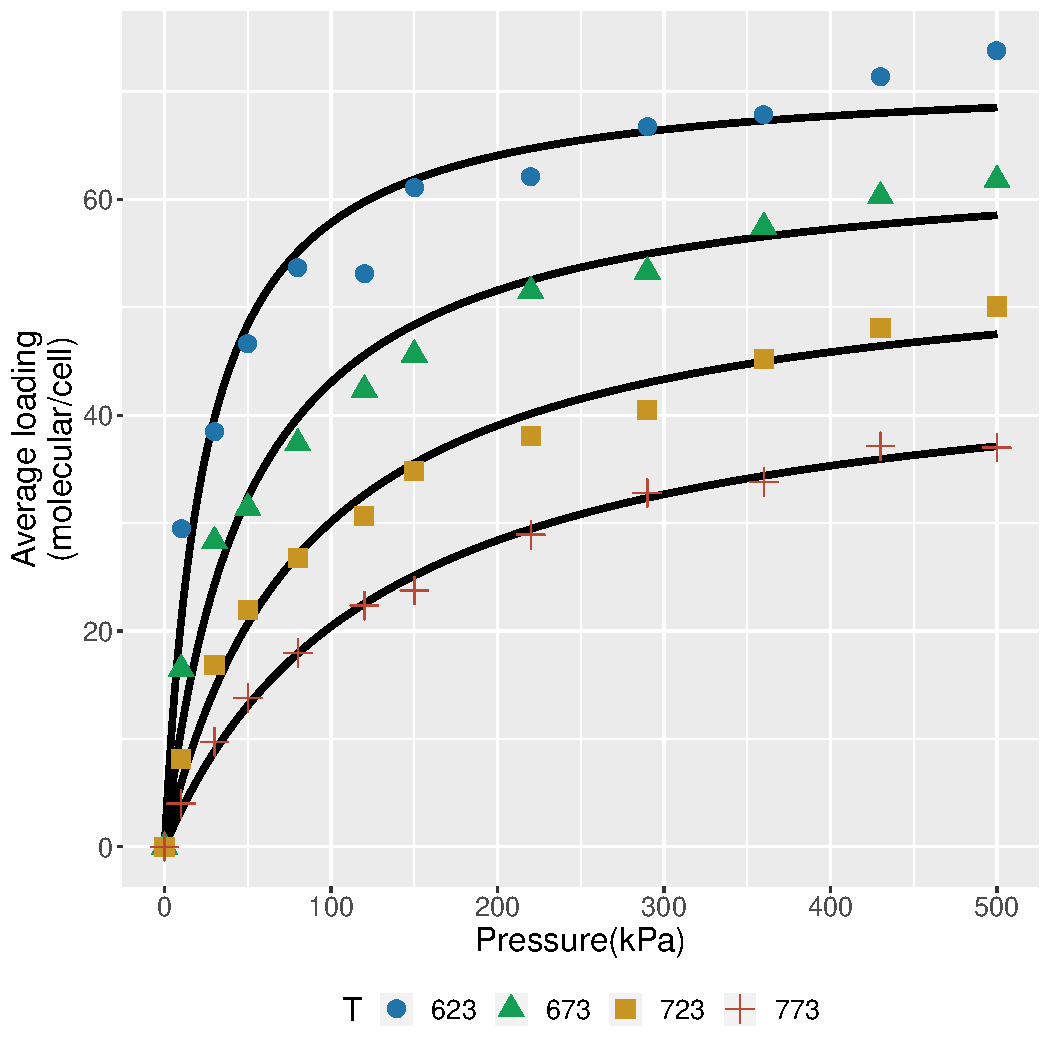
\includegraphics[width=2.7in]{figure/Adsorption/MacroPore20A.pdf}
    %\caption{fig2}
    \end{minipage}%
    }%
    \subfigure[丁酸甲酯在60Å介孔]{
    \begin{minipage}[t]{0.5\linewidth}
    \centering
    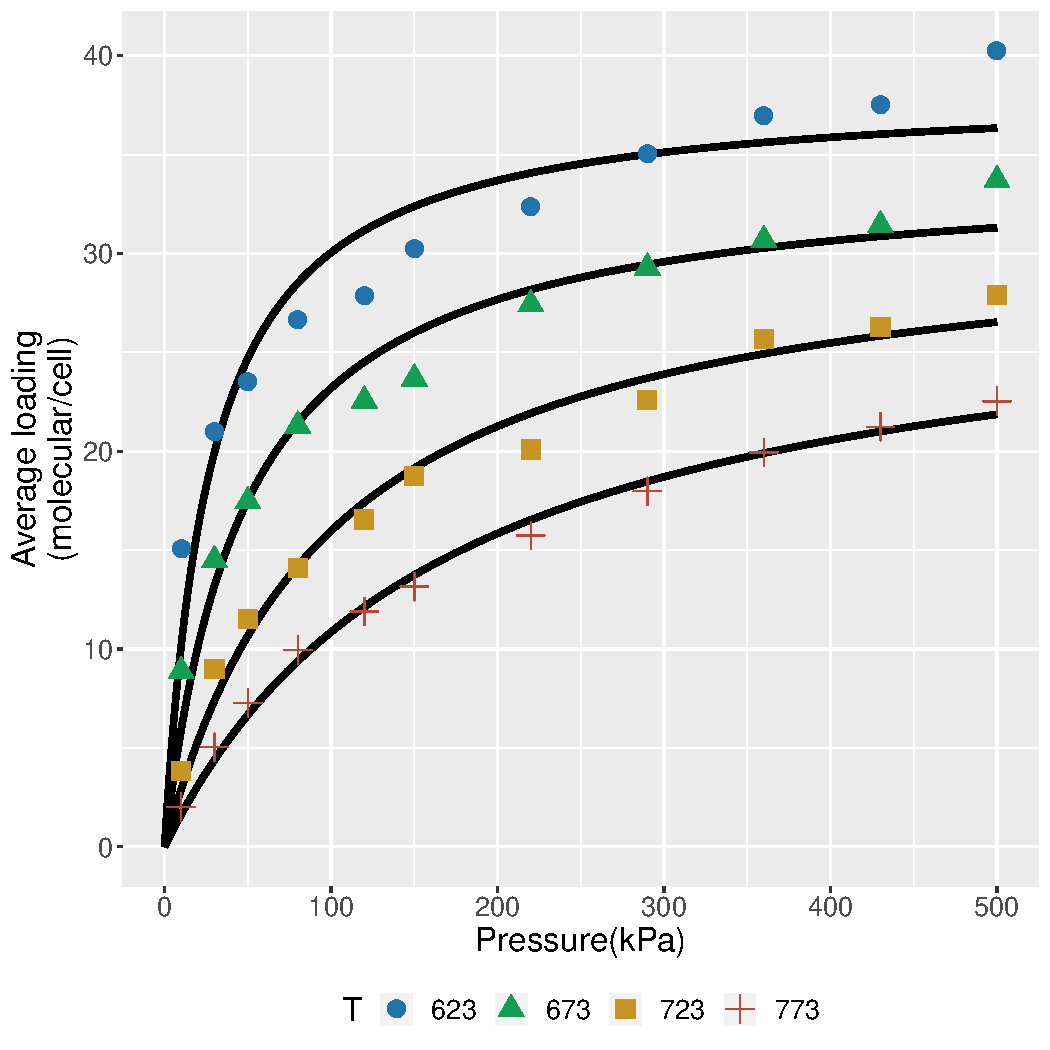
\includegraphics[width=2.7in]{figure/Adsorption/MacroPore60Anew.pdf}
    %\caption{fig2}
    \end{minipage}%
    }%
    \caption{丁酸甲酯和丁烯酸甲酯在微介孔H-ZSM-5分子筛的吸附等温线图}
    \label{fig:sA}
\end{figure}


\par{从\reffig{fig:sA}中可以看出:丁酸甲酯和丁烯酸甲酯的吸附等温线属于\uppercase\expandafter{\romannumeral1}型,满足朗格缪尔吸附方程,说明均为单层吸附,且吸附分子与分子筛之间的作用力占主导地位。对数据采用 \ref{郎格缪尔吸附} 所介绍的Langmuir公式进行拟合,公式如下:}
\begin{equation}
    V_{\mathrm{m}}=V_{\mathrm{m}^{\mathrm{a}}} \frac{b P}{1+b P}
\end{equation}
\par{式中:$V_{\mathrm{m}}$为平衡吸附量,$V_{\mathrm{m}^{a}}$ 为饱和吸附量,b为吸附平衡常数,P为压力。}
\par{拟合结果见\reftab{tab:sA}。}

\begin{table}[H]
	\small
	\centering
	\caption{在微介孔H-ZSM-5分子筛内丁酸甲酯和丁烯酸甲酯Langmuir公式拟合数据对比表}
	\begin{tabular}{p{2cm}<{\centering}p{2cm}<{\centering}p{1cm}<{\centering}p{4cm}<{\centering}p{2cm}<{\centering}p{2cm}<{\centering}}
        \toprule
        吸附质&孔径&\makecell*[c]{温度\\(K)}&\makecell*[c]{饱和吸附量\\(吸附分子数/超胞)}&\makecell*[c]{饱和吸附量\\(mmol/g)}&b\\
        \midrule
        \multirow{12}{*}{丁酸甲酯}&\multirow{4}{*}{微孔}&623&77.78&1.1238&0.1448\\
        &&673&71.83&1.0378&0.0559\\
        &&723&65.51&0.9465&0.0258\\
        &&773&60.22&0.8701&0.0115\\
        \cline{2-6}
        &\multirow{4}{*}{20Å介孔}&623&71.84&1.3502&0.0413\\
        &&673&64.31&1.2087&0.0203\\
        &&723&55.52&1.0435&0.0119\\
        &&773&46.66&0.8769&0.0078\\
        \cline{2-6}
        &\multirow{4}{*}{60Å介孔}&623&38.35&1.2271&0.0362\\
        &&673&34.31&1.0978&0.0209\\
        &&723&31.79&1.0172&0.0101\\
        &&773&29.28&0.9368&0.0059\\
        \hline
        \multirow{4}{*}{丁烯酸甲酯}&\multirow{4}{*}{微孔}&623&82.97&1.1987&0.2050\\
        &&673&79.44&1.1477&0.0642\\
        &&723&74.02&1.0694&0.0245\\
        &&773&64.77&0.9358&0.0132\\
		\bottomrule
	\end{tabular}
	\label{tab:sA}
\end{table}

\par{因为60Å介孔采用4×4×3的超胞进行模拟,所以为了和2×2×3超胞的微孔和20Å介孔在相同体积的条件下进行比较,60Å介孔的吸附量要除以四。}
\par{从\reftab{tab:sA}中可知,随着孔径的增大,丁酸甲酯的饱和吸附量越来越小。这是因为分子筛随着孔径的增大,相同体积下的活性吸附位(B位酸)数量减小(吸附位密度减小),以及微孔孔道(一般吸附位)数量减小,导致总的吸附位数量减小,从而丁酸甲酯的吸附量减小。而随着孔径的增大,单位质量下的分子筛吸附的丁酸甲酯分子的数量先增大,后减小,20Å介孔的吸附量最大,说明单位质量的20Å介孔的吸附效率最高,并不是孔径越大越好。在相同孔径的条件下,随着温度的增高,饱和吸附量减小,这是因为吸附是放热过程,低温有利于吸附。Langmuir公式中的b(吸附平衡常数)随着温度增大而减小,这是因为吸附平衡常数等于吸附速率常数比上解吸速率常数,随着温度的增高,吸附速率常数没有解吸速率常数增加得快。而在相同温度下,随着分子筛孔径的增大,丁酸甲酯的b(吸附平衡常数)减小,说明微孔与吸附分子之间的作用力更强,能更快的达到吸附饱和。}
\par{从\reftab{tab:sA}还可以看出,在623K$\sim$773K范围内,丁烯酸甲酯的饱和吸附量和b(吸附平衡常数)比丁酸甲酯的大,这是因为双键的存在,使丁烯酸甲酯具有更大的极性,而H-ZSM-5分子筛也是极性的,当吸附分子靠近吸附剂时,二者的电子结构发生变化而产生偶极矩,相互之间的主要作用力变成了更强的定向力和诱导力,从而吸附了更多的丁烯酸甲酯。}
\par{本文还研究了0$\sim$500kPa下乙酸甲酯到戊酸甲酯的吸附,随着吸附分子碳链长度的增加,脂肪酸甲酯在H-ZSM-5分子筛上的吸附也具有一定的规律。\reffig{fig:C2_C5}展示了不同碳链长度的脂肪酸甲酯在H-ZSM-5分子筛的吸附等温线。}

\begin{figure}[H]
    \centering
        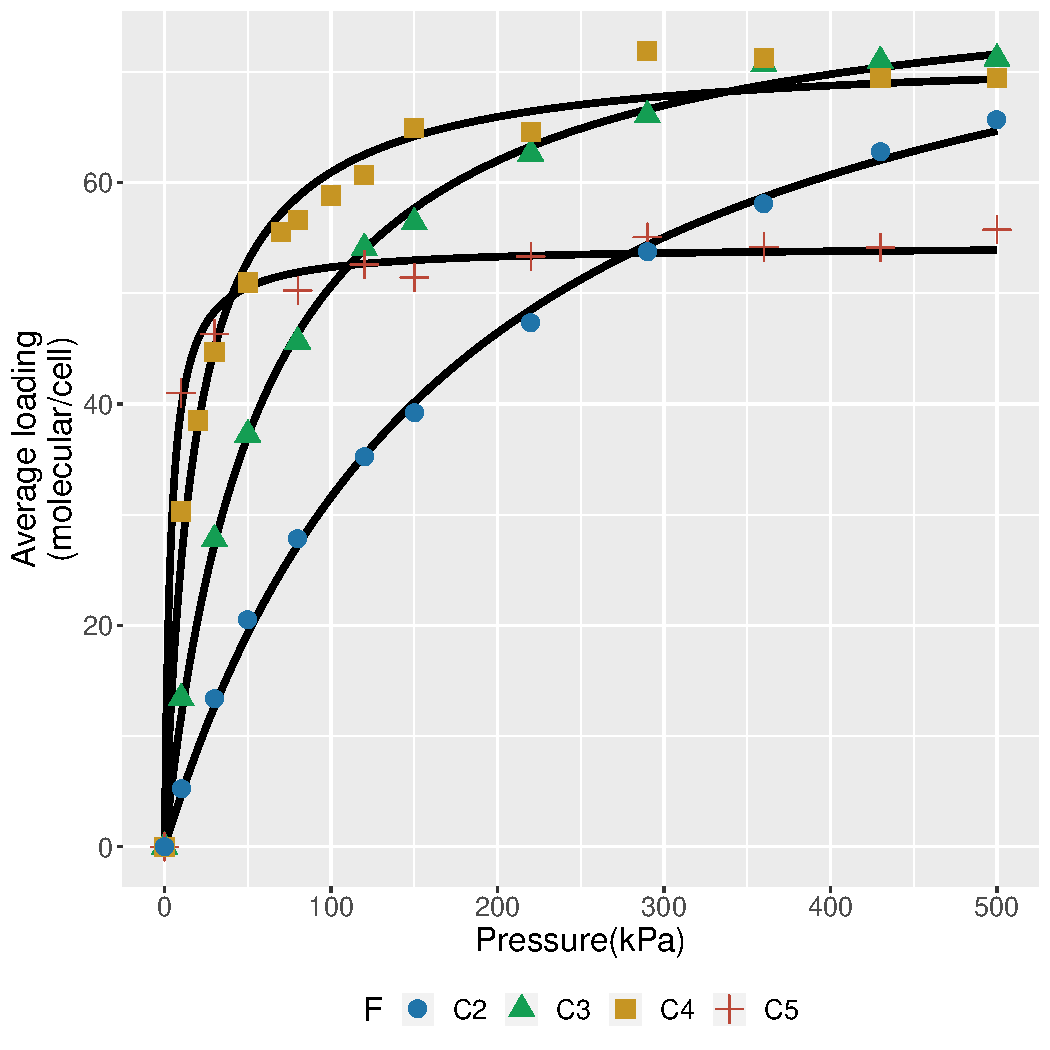
\includegraphics[width=0.5\linewidth]{figure/Adsorption/length.pdf}
    \caption{乙酸甲酯至戊酸甲酯在微孔H-ZSM-5分子筛内的吸附等温线图}
    \label{fig:C2_C5}
\end{figure}
\par{从\reffig{fig:C2_C5}可以看到,随着碳链长度的增加,脂肪酸甲酯在HZSM-5分子筛上的吸附量下降,b(吸附平衡常数)不断增大,通过 \ref{checking} 可知,油酸甲酯(十八烷酸甲酯)的b高达2.92。这是因为链长越大,分子筛对它的范德华力越大,就能越快地达到吸附平衡,但链长增大所引起的空间位阻的增大导致了其吸附量减小。具体拟合数据见\reftab{tab:C2_C5}。}
\begin{table}[H]
	\small
	\centering
	\caption{不同链长的脂肪酸甲酯Langmuir公式拟合数据对比表}
	\begin{tabular}{p{3cm}<{\centering}p{4cm}<{\centering}p{2.5cm}<{\centering}p{2.5cm}<{\centering}}
        \toprule
        分子&\makecell*[c]{饱和吸附量\\(吸附分子数/超胞)}&\makecell*[c]{饱和吸附量\\(mmol/g)}&b\\
        \midrule
        乙酸甲酯&87.59&1.2655&0.0056\\
        丙酸甲酯&79.84&1.1535&0.0173\\
        丁酸甲酯&71.83&1.0378&0.0559\\
        戊酸甲酯&54.29&0.7844&0.2703\\
		\bottomrule
	\end{tabular}
	\label{tab:C2_C5}
\end{table}
\subsubsection{等量吸附热}
\par{等量吸附热是固体吸附气体过程中衡量吸附质分子吸附性能的一个重要参数,被定义为吸附质分子在由游离的气体分子状态转为被吸附剂分子吸附时的状态所放出的热量。}
\par{在巨正则蒙特卡洛法(GCMC)的模拟中,等量吸附热Q是依据下式计算得出:}
\begin{equation}
    Q=R T-\frac{\left\langle N U_{N}\right\rangle-\langle N\rangle\left\langle U_{N}\right\rangle}{\left\langle N^{2}\right\rangle\langle N\rangle^{2}}
    \end{equation}
\par{式中:$N$为吸附分子数;$R$为体系开式温度;$R$为理想气体常数;$U_N$为吸附相势能;$ \langle \rangle$为系综平均。}

\par{\reffig{fig:sH1}为丁酸甲酯分子在673K,微介孔H-ZSM-5分子筛中的等量吸附热随吸附量和压力的变化图。}
\begin{figure}[H]
    \centering

    \subfigure[等量吸附热随压力变化图]{
        \begin{minipage}[t]{0.5\linewidth}
        \centering
        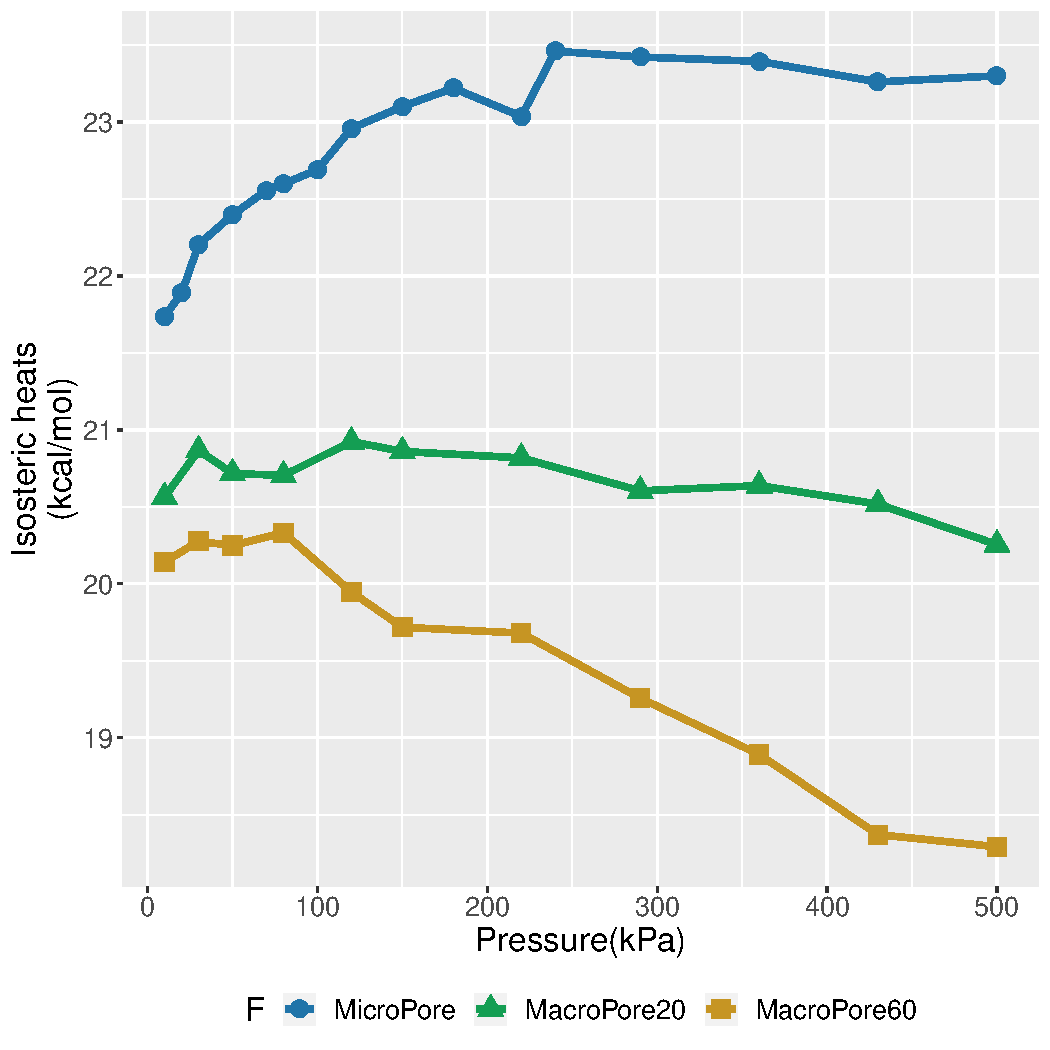
\includegraphics[width=2.8in]{figure/Adsorption/Heat673.pdf}
        %\caption{fig1}
        \end{minipage}%
    }%
    \subfigure[等量吸附热随吸附量变化图]{
        \begin{minipage}[t]{0.5\linewidth}
        \centering
        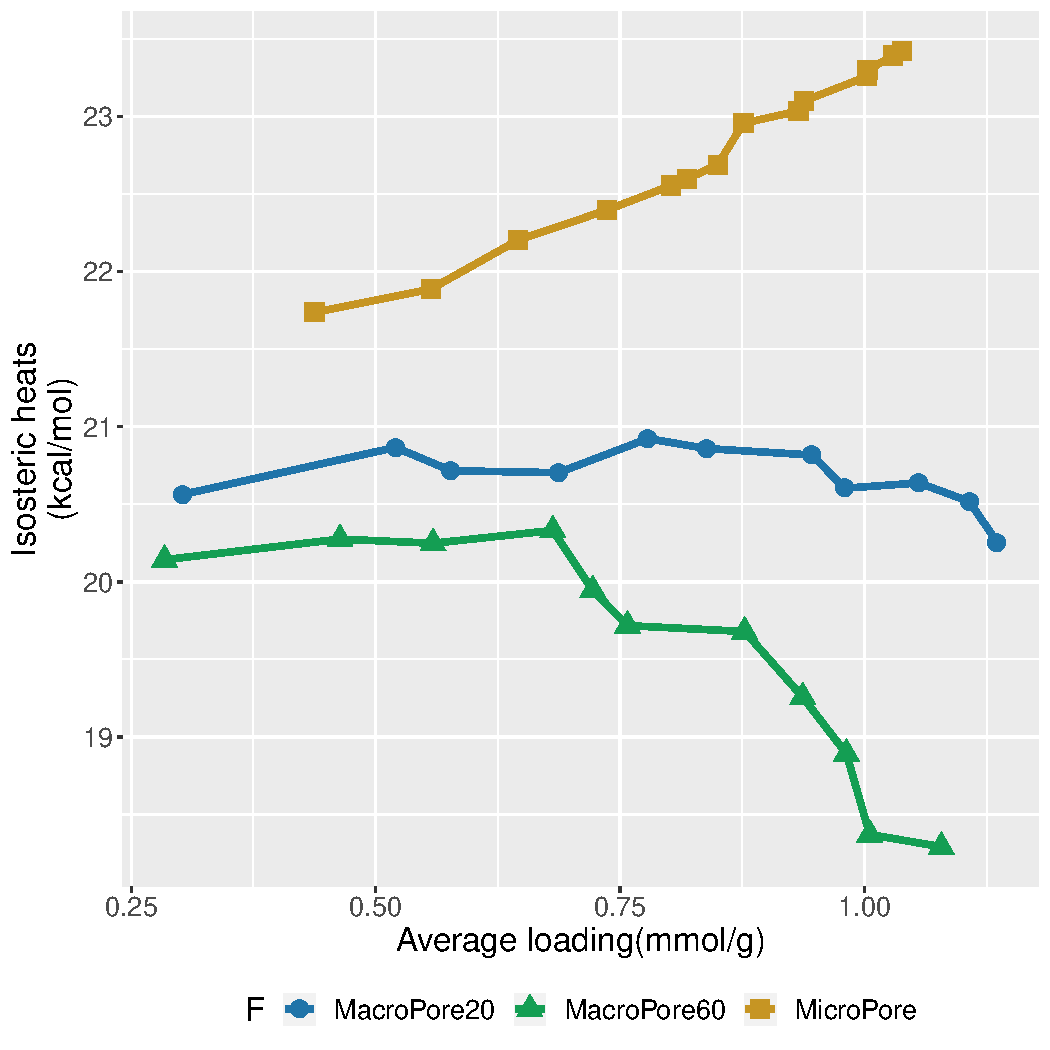
\includegraphics[width=2.8in]{figure/Adsorption/111.pdf}
        %\caption{fig1}
        \end{minipage}%
    }%
    \caption{丁酸甲酯在673K下不同孔径分子筛中的等量吸附热随吸附量和压力的变化图}
    \label{fig:sH1}
\end{figure}
\par{从\reffig{fig:sH1}中可以看出,在相同压力或者吸附量的条件下,60Å介孔 < 20Å介孔<微孔的等量吸附热,说明孔径越大,等量吸附热越小。翟冬\cite{翟冬2011C4}认为吸附热主要受两部分作用力影响:吸附质与吸附剂之间的相互作用力以及吸附剂分子之间的相互作用力。因为从 \ref{吸附等温线} 可知,吸附分子与微孔之间的作用力大于与介孔的(在微孔中的吸附平衡常数比在介孔的大),所以微孔的更加稳定,放出的热就更多。}
\par{在微孔分子筛中,随着压力的增大,等量吸附热逐渐增大,直到达到最大值,随着吸附量的增大,等量吸附热线性增大。因为当吸附量增加时,吸附质分子之间距离的变小,吸附质分子之间的相互作用将越来越大,单位数量的吸附质之间的作用力引起的吸附热将越来越大,但吸附分子与吸附剂之间的相互作用并不会随吸附量的增大而增大,所以丁酸甲酯在微孔内的吸附热的变化本质上是由于吸附质分子之间的相互作用增大而引起的。}
\par{而介孔的等量吸附热随着压力或者吸附量的增大,等量吸附热先增大后减小,有一个最大值。这是因为在分子筛中引入介孔为吸附分子提供了较短的扩散路径和较高的扩散速率\cite{liu2012adsorption}。在低压下丁酸甲酯在介孔分子筛孔道吸附固定的效率较高,优先占据活性吸附位(B位酸),放出较高吸附热量\cite{2017介孔材料吸附气相多环芳烃实验及分子模拟研究},再加上上文所说的吸附量增加,吸附分子之间作用力增大,等量吸附热增大,所以刚开始等量吸附热会随吸附量(压力)增大而增大;而随着压力升高,吸附量增加量减小,逐渐达到饱和,吸附分子之间距离减小所增加的吸附热的影响减小,活性位点(B位酸)也逐渐被占据完,吸附质分子转向一般的吸附位点(孔道),放出的吸附热下降,吸附量增加所导致的吸附热增加量小于减少量,于是等量吸附热随着吸附量增加而下降。}
\par{而60Å介孔的等量吸附热最高点时的压力小于20Å介孔的是因为在60Å介孔分子筛中,到活性位点的路径更加短,而且在相同体积的条件下,60Å介孔的活性吸附位(B位酸)的个数原小于20Å介孔的个数,所以压力更低(吸附量更少)的条件下,即可完成所有活性吸附位点的吸附。}


\par{\reffig{fig:sH2}展示了温度对等量吸附热的影响,从图中可以看出温度越高,吸附热越小,并且在相同吸附量下,介孔中的吸附热比微孔的对温度更加敏感。因为吸附热是当气体分子固定在吸附位时,吸附分子因速度变慢导致动能减小,从而释放热量,而温度升高,吸附分子运动变剧烈,所以转化的动能(吸附热)变少,而介孔分子筛中的吸附位在介孔周围,附着在吸附位上的吸附分子受到的空间位阻相对较小,所以随着温度的增大,运动幅度相较微孔增加得更大,动能增加量更大,于是释放的热量减少得更多。}

\begin{figure}[H]
    \centering

    \subfigure[微孔压力]{
    \begin{minipage}[t]{0.5\linewidth}
    \centering
    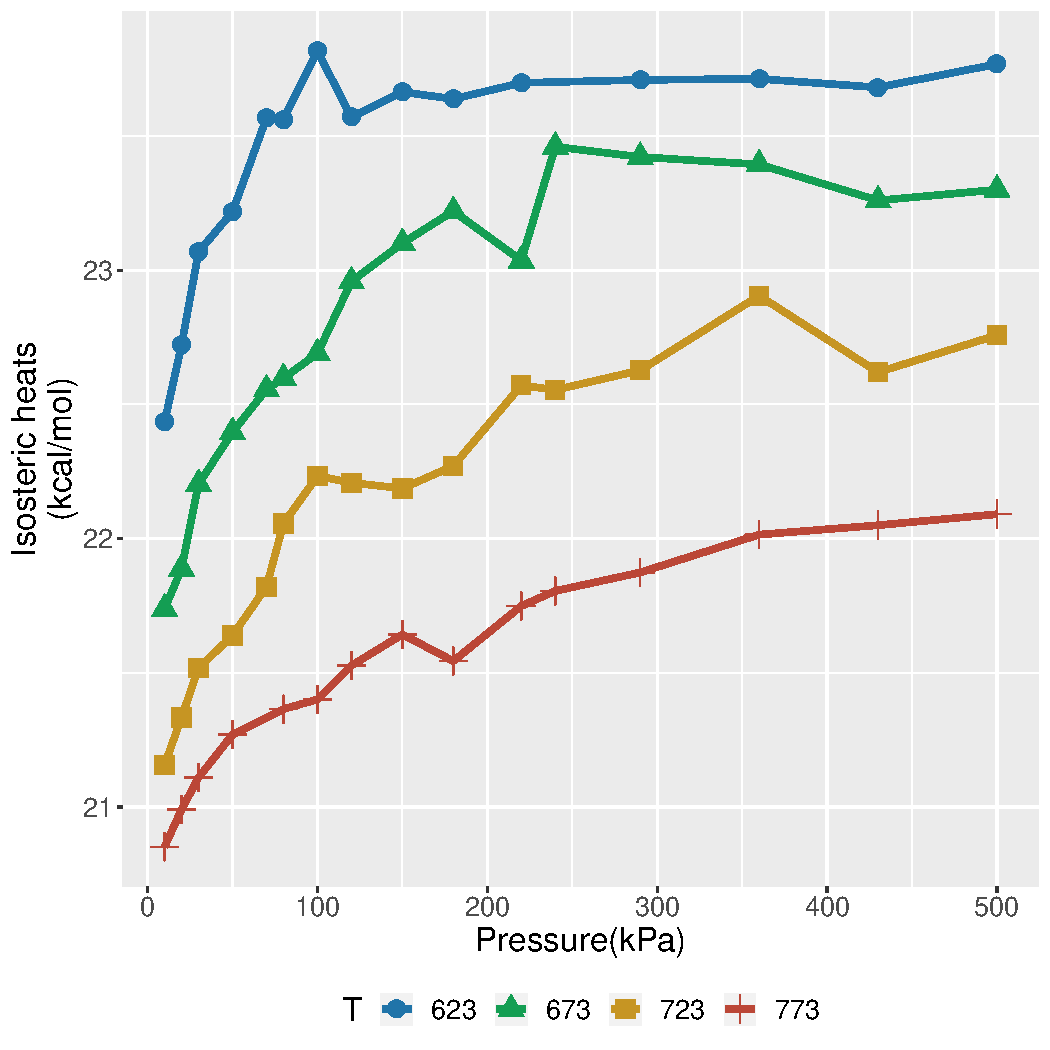
\includegraphics[width=2.7in]{figure/Adsorption/MicroPoreH.pdf}
    %\caption{fig1}
    \end{minipage}%
    }%
    \subfigure[微孔吸附量]{
    \begin{minipage}[t]{0.5\linewidth}
    \centering
    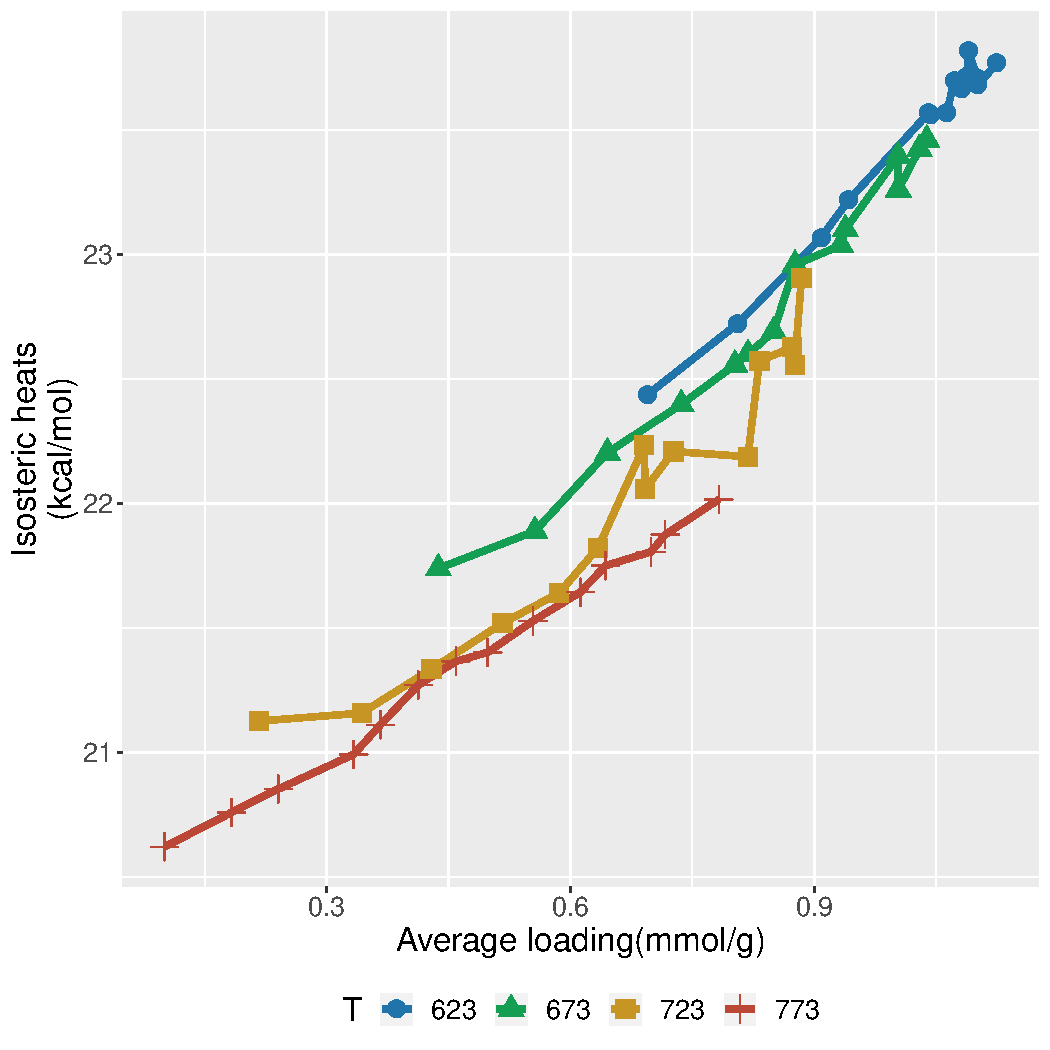
\includegraphics[width=2.7in]{figure/Adsorption/222MM.pdf}
    %\caption{fig2}
    \end{minipage}%
    }%

    \subfigure[20Å介孔压力]{
    \begin{minipage}[t]{0.5\linewidth}
    \centering
    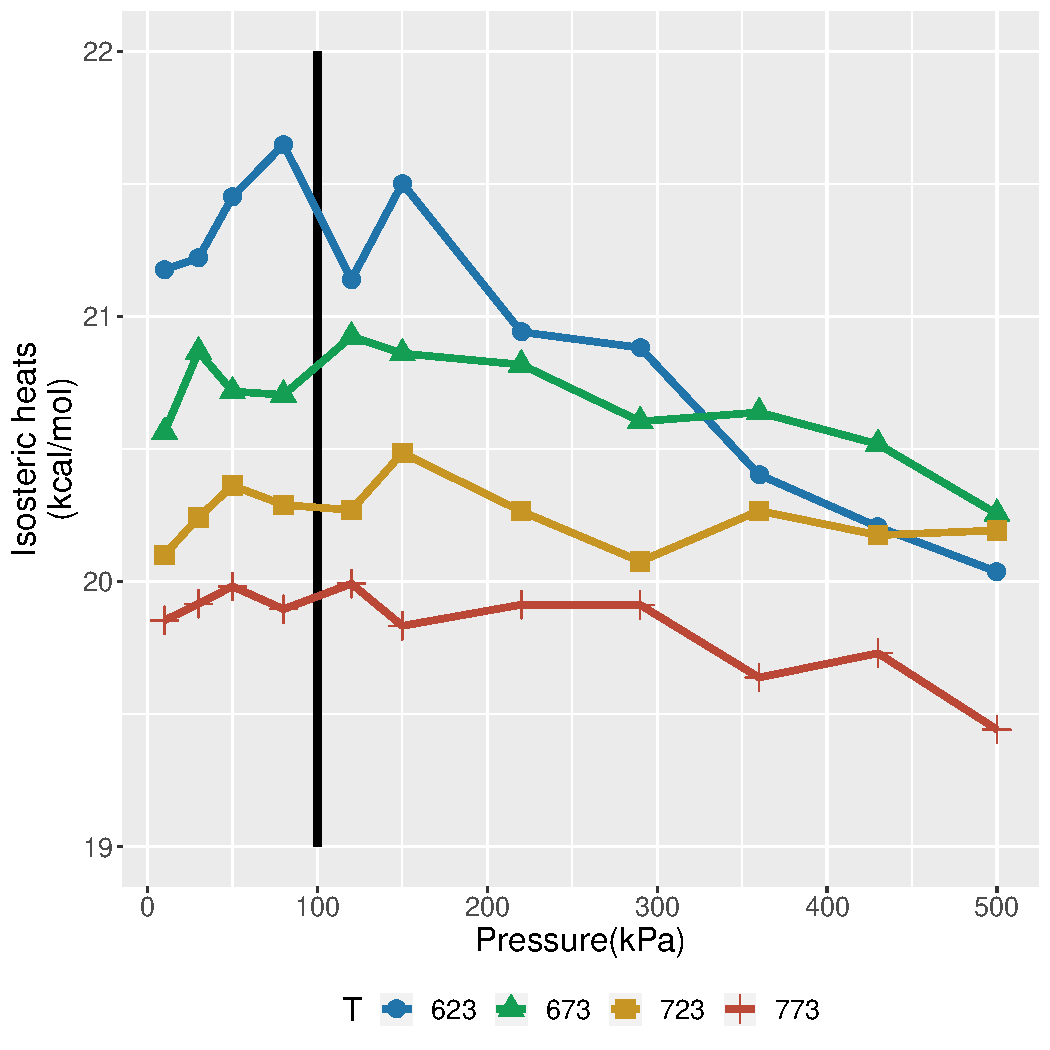
\includegraphics[width=2.7in]{figure/Adsorption/MacroPore20H.pdf}
    %\caption{fig2}
    \end{minipage}%
    }%
    \subfigure[20Å介孔吸附量]{
    \begin{minipage}[t]{0.5\linewidth}
    \centering
    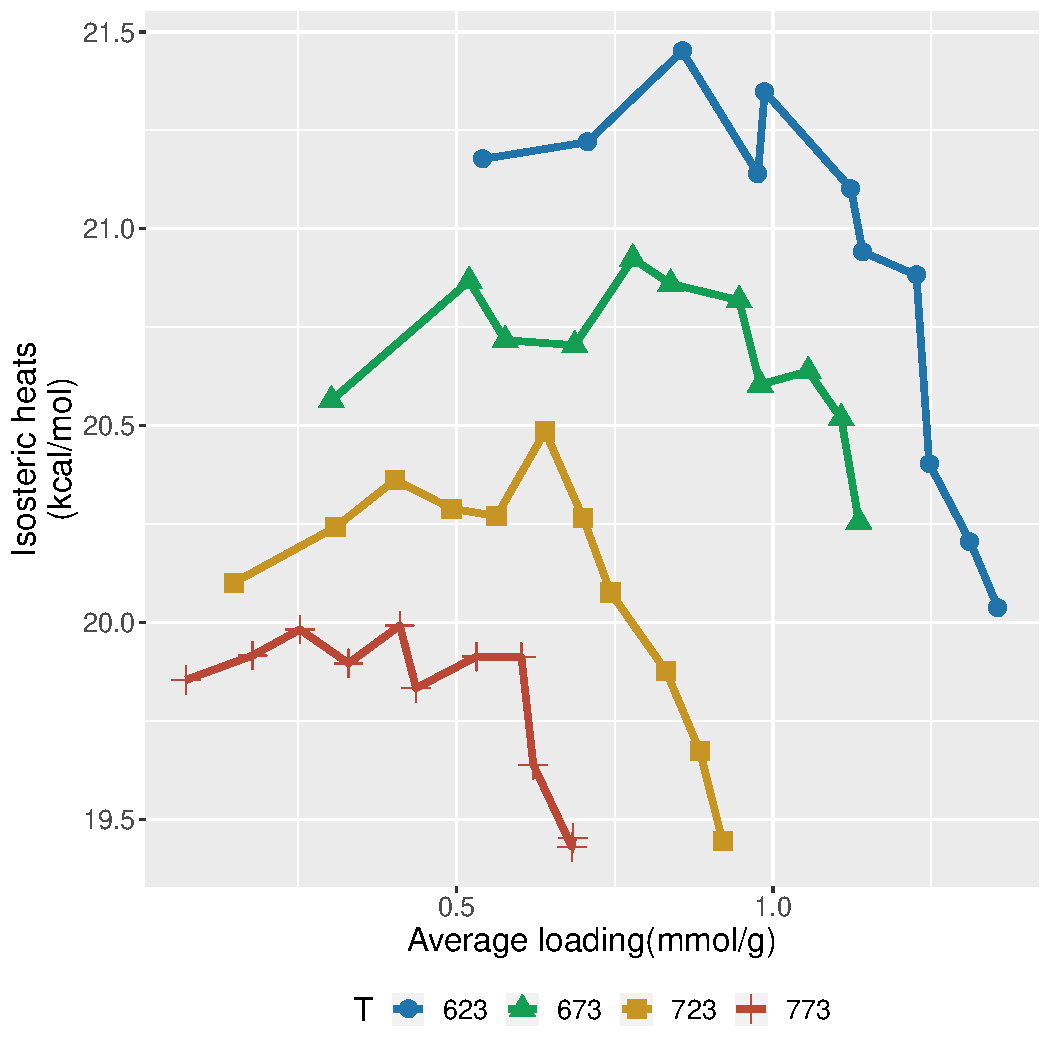
\includegraphics[width=2.7in]{figure/Adsorption/222M20.pdf}
    %\caption{fig2}
    \end{minipage}%
    }%

    \subfigure[60Å介孔压力]{
    \begin{minipage}[t]{0.5\linewidth}
    \centering
    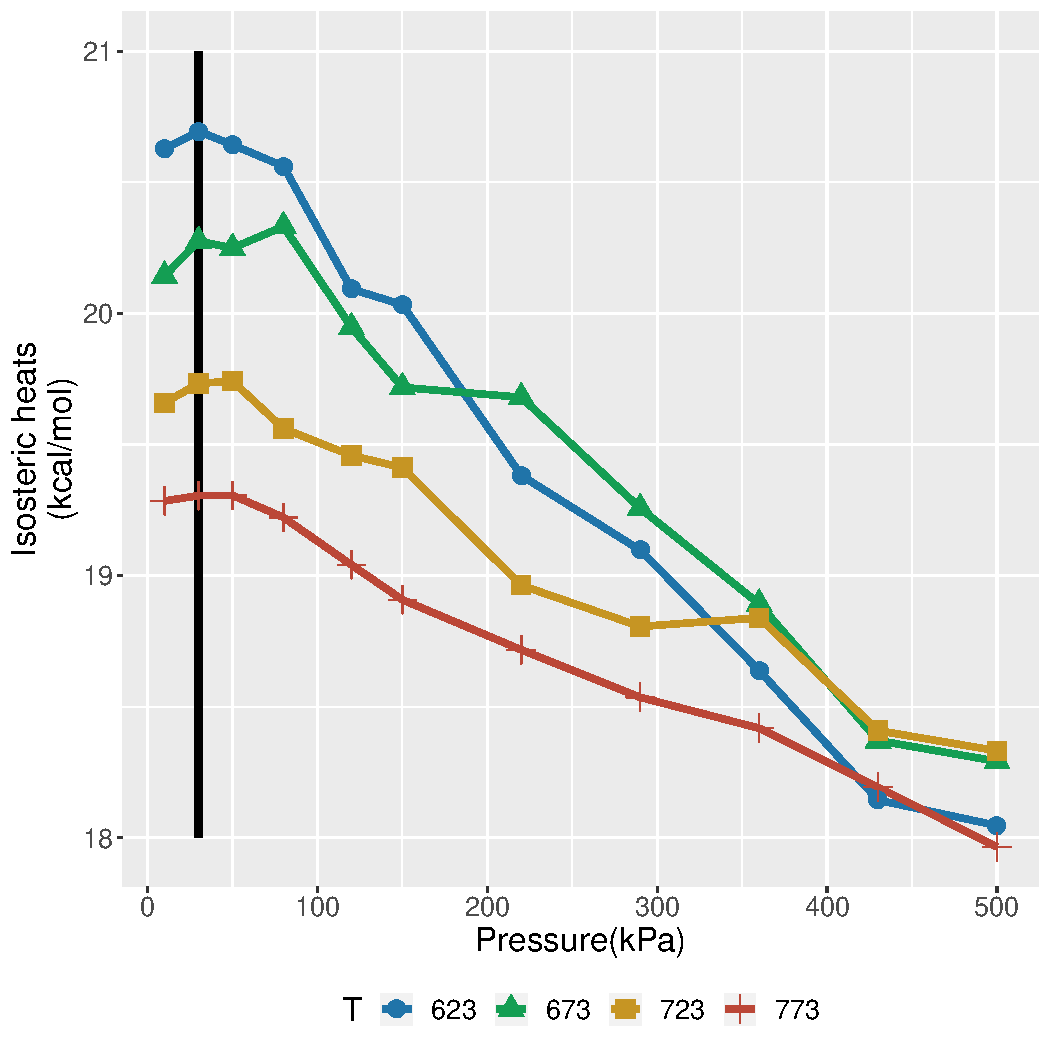
\includegraphics[width=2.7in]{figure/Adsorption/MacroPore60H.pdf}
    %\caption{fig2}
    \end{minipage}%
    }%
    \subfigure[60Å介孔吸附量]{
    \begin{minipage}[t]{0.5\linewidth}
    \centering
    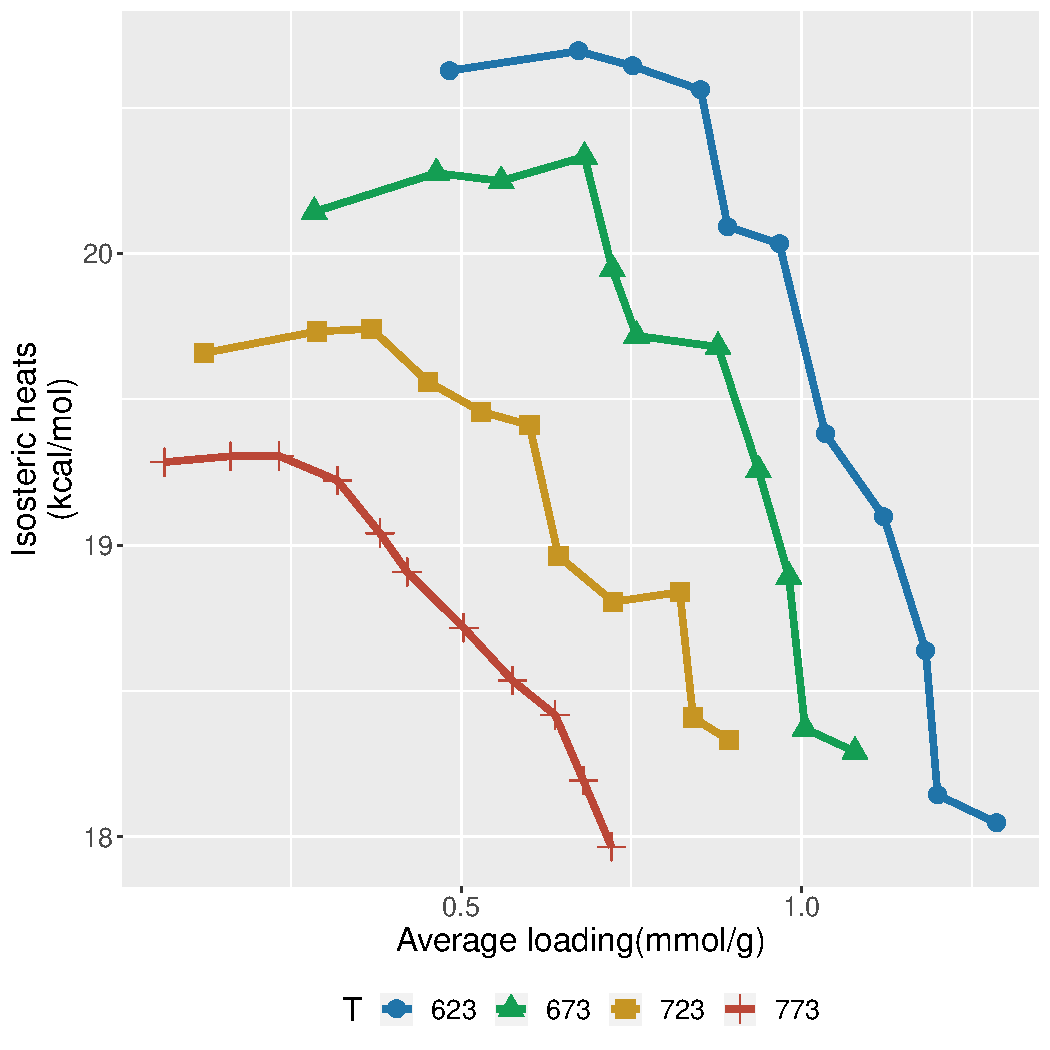
\includegraphics[width=2.7in]{figure/Adsorption/222M60.pdf}
    %\caption{fig2}
    \end{minipage}%
    }%
    \caption{丁酸甲酯在不同温度下的等量吸附热随压力和吸附量的变化图}
    \label{fig:sH2}
\end{figure}
\par{通过\reffig{fig:sH2}还发现在介孔中的等量吸附热最大值所对应的压力几乎不随温度发生变化,孔径越大,结果越明显。这是因为在60Å介孔的条件下,饱和吸附量从623K到773K下降了23.7\%,而20Å介孔下降了35.1\%,说明在相同压力下,在20Å介孔中的吸附量对温度更加敏感,而吸附量改变,等量吸附热则会改变,所以当温度改变时,在对温度相对不敏感的60Å介孔中的等量吸附热变化较小。}


% \par{本文计算了不同链长的脂肪酸甲酯在微孔H-ZSM-5上的等量吸附热随吸附量的变化曲线。如\reffig{fig:C2_C5H}所示,随着吸附量的增大,等量吸附热线性增大。这是因为随着吸附量的增大,吸附质分子之间的距离变短,从而吸附质分子之间的作用力变大,放出更多的热量,从而单位数量的吸附质分子之间的作用力引起的热量更大,而吸附质与吸附剂之间的作用力并不会随着吸附质分子数量的增大而增大,所以最后随着吸附量的增大,等量吸附热变大。}

% \begin{figure}[H]
%     \centering
%         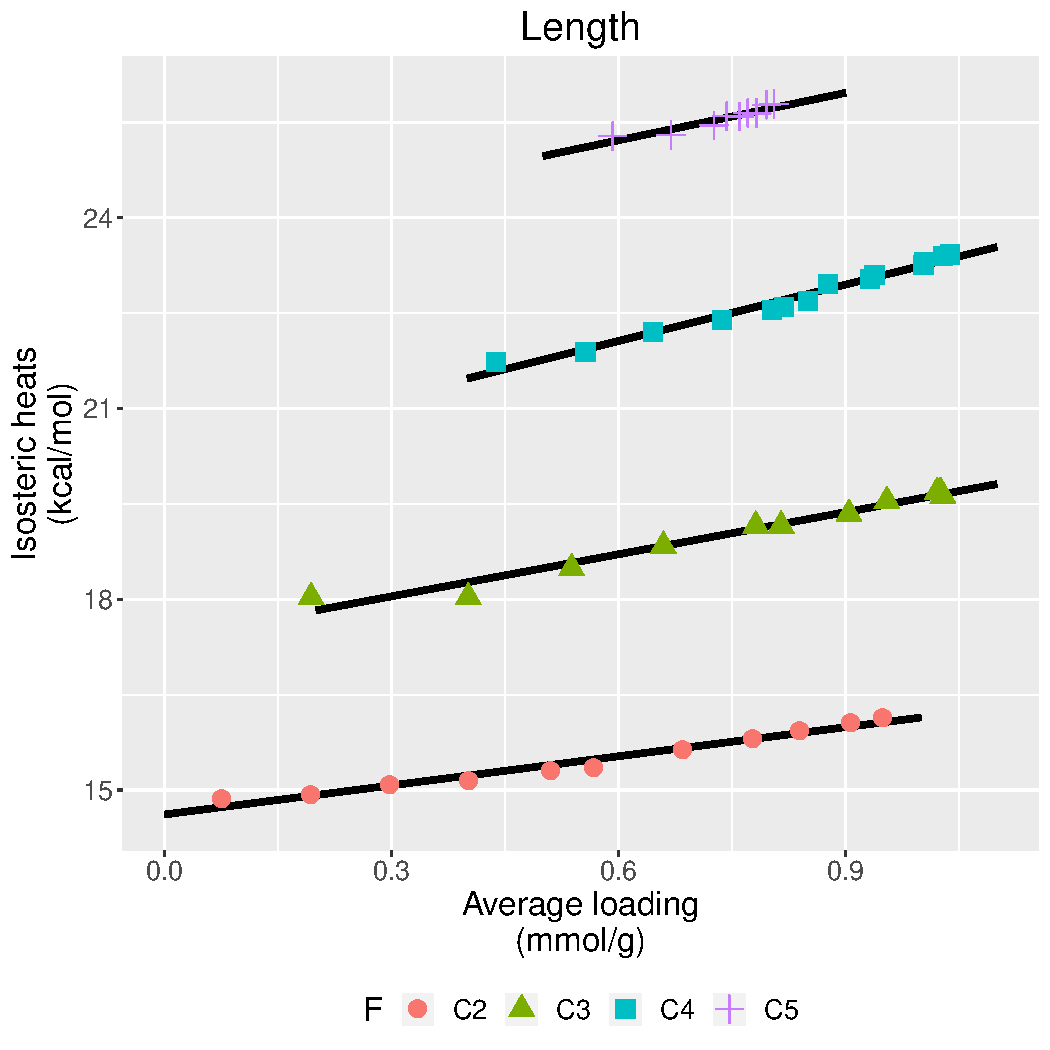
\includegraphics[width=0.6\linewidth]{figure/Adsorption/lengthheat.pdf}
%     \caption{乙酸甲酯至戊酸甲酯在微孔H-ZSM-5分子筛内的吸附热随吸附量的变化曲线图}
%     \label{fig:C2_C5H}
% \end{figure}
% \par{从\reffig{fig:C2_C5H}还发现,吸附热与链长呈直线关系,所以选取吸附量为0.6mmol/mg时的吸附热与链长作图,如所示\reffig{fig:C2_C5h}所示。R$^2$=0.9999,且每增加一个亚甲基,等量吸附热变增加3.24kcal/mol,约13.55kJ/mol。这个现象与实验报道的烷烃链长和吸附热呈线性关系,且每增加一个亚甲基等量吸附热就增加10kJ/mol\cite{yang1986use}的结果相似。}

% \begin{figure}[H]
%     \centering
%         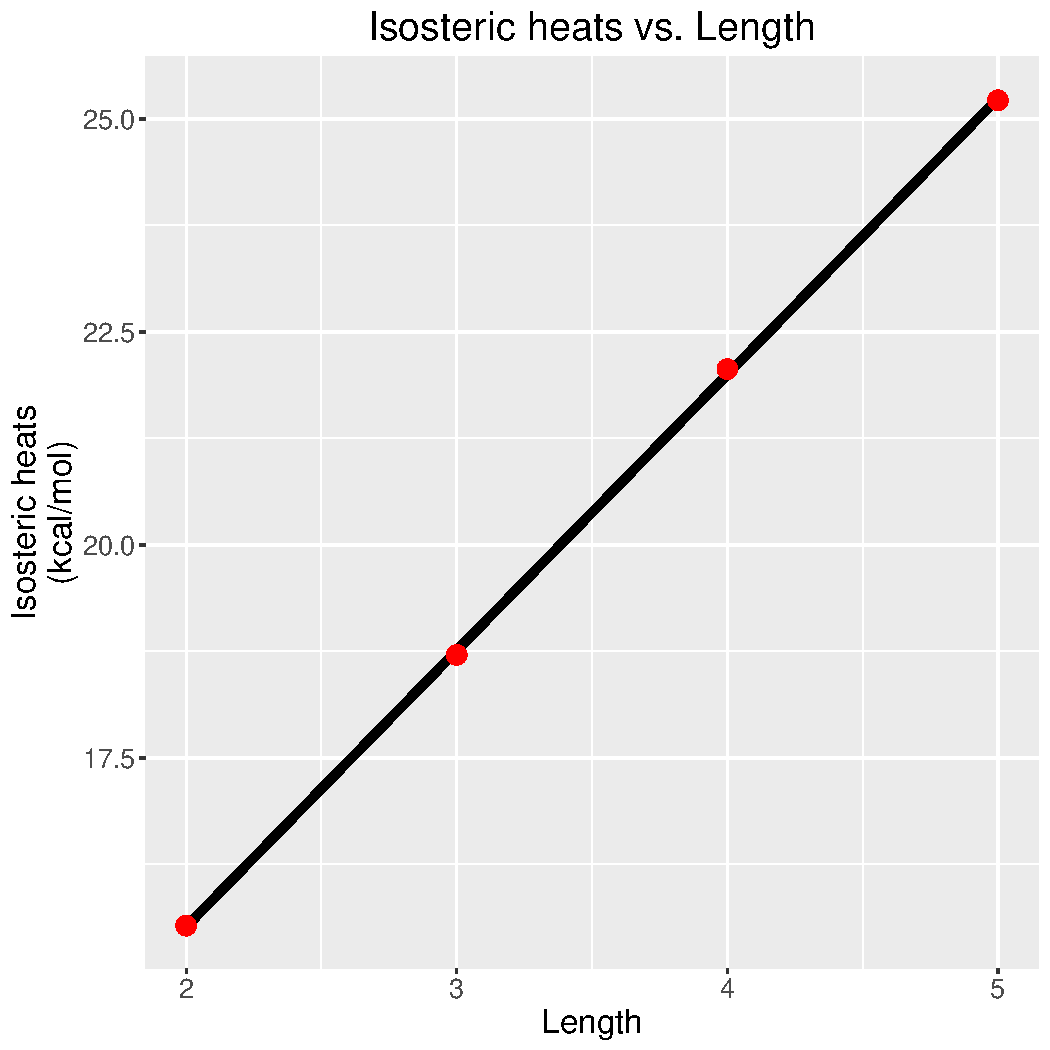
\includegraphics[width=0.6\linewidth]{figure/Adsorption/lengthH.pdf}
%     \caption{在微孔H-ZSM-5分子筛内的等量吸附热随吸附质链长的变化曲线}
%     \label{fig:C2_C5h}
% \end{figure}


\subsubsection{吸附位}
\par{本文研究了压力对吸附位置的影响,选取10kPa作为低压,1000kPa作为高压,温度取673K,结果如\ref{fig:loaction}所示。}


\begin{figure}[H]
    \centering

    \subfigure[低压A方向]{
    \begin{minipage}[t]{0.3333\linewidth}
    \centering
    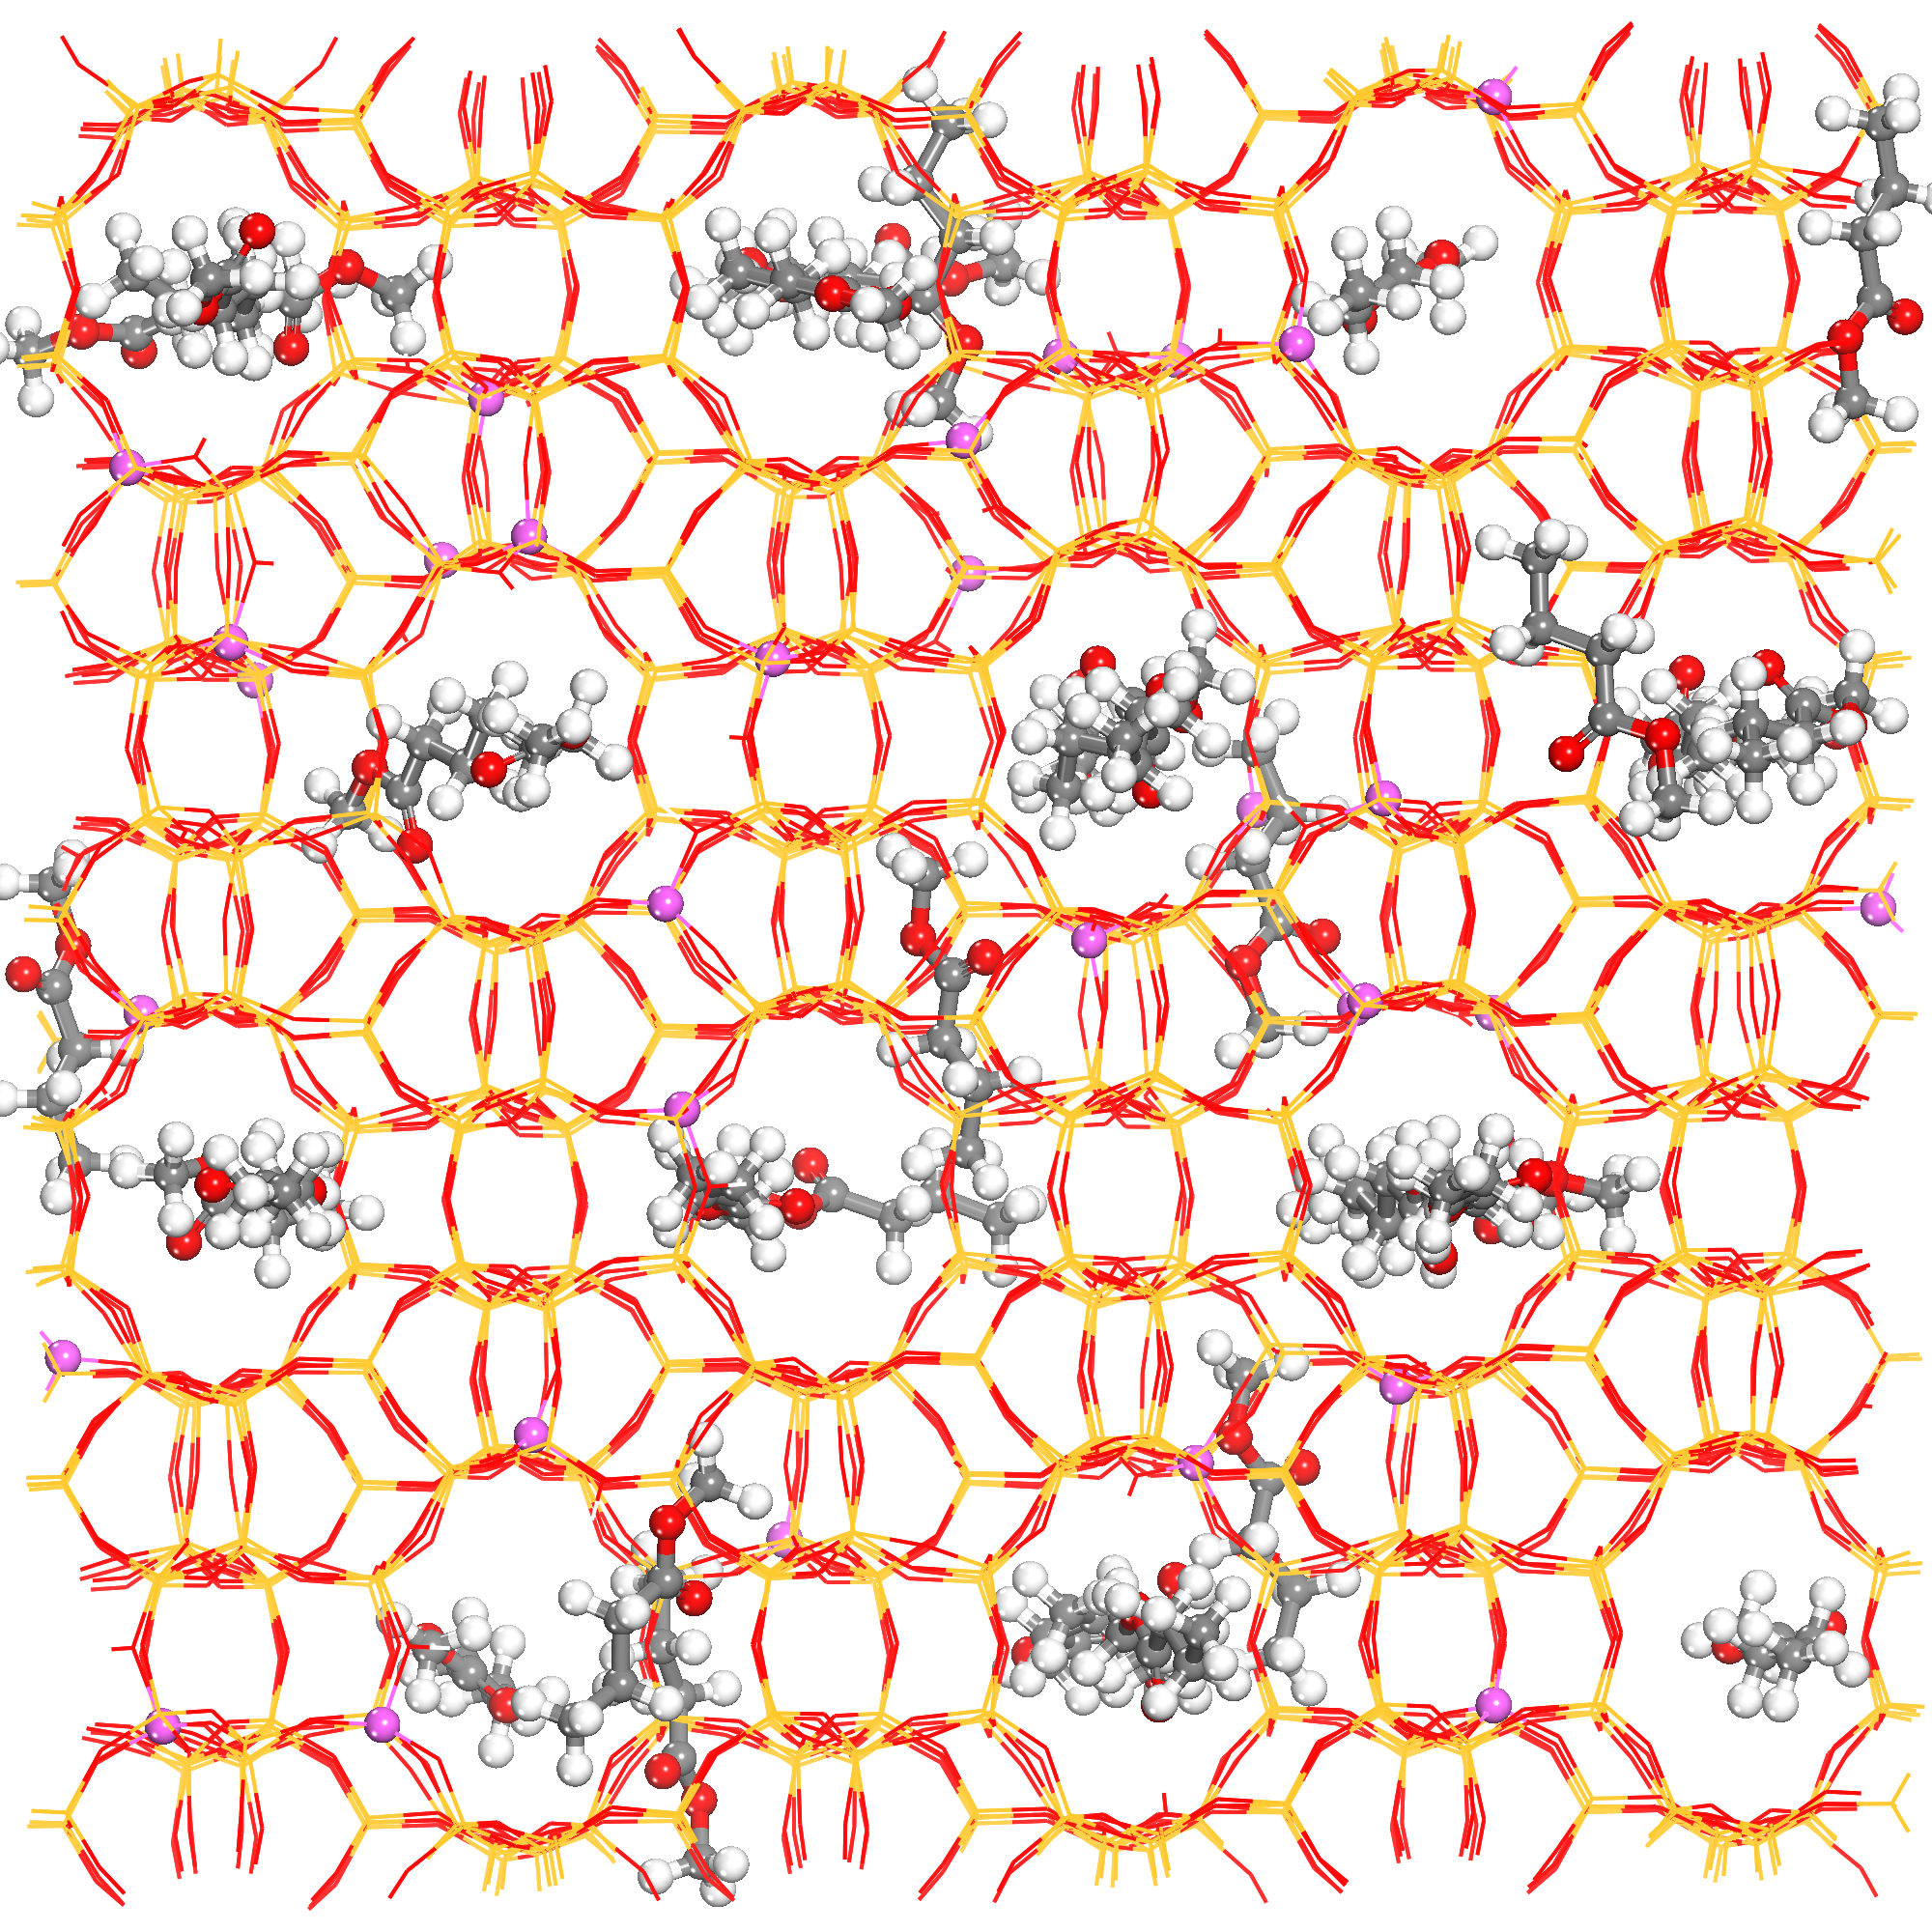
\includegraphics[width=1.8in]{figure/Adsorption/lowA.png}
    %\caption{fig1}
    \end{minipage}%
    }%
    \subfigure[低压B方向]{
    \begin{minipage}[t]{0.3333\linewidth}
    \centering
    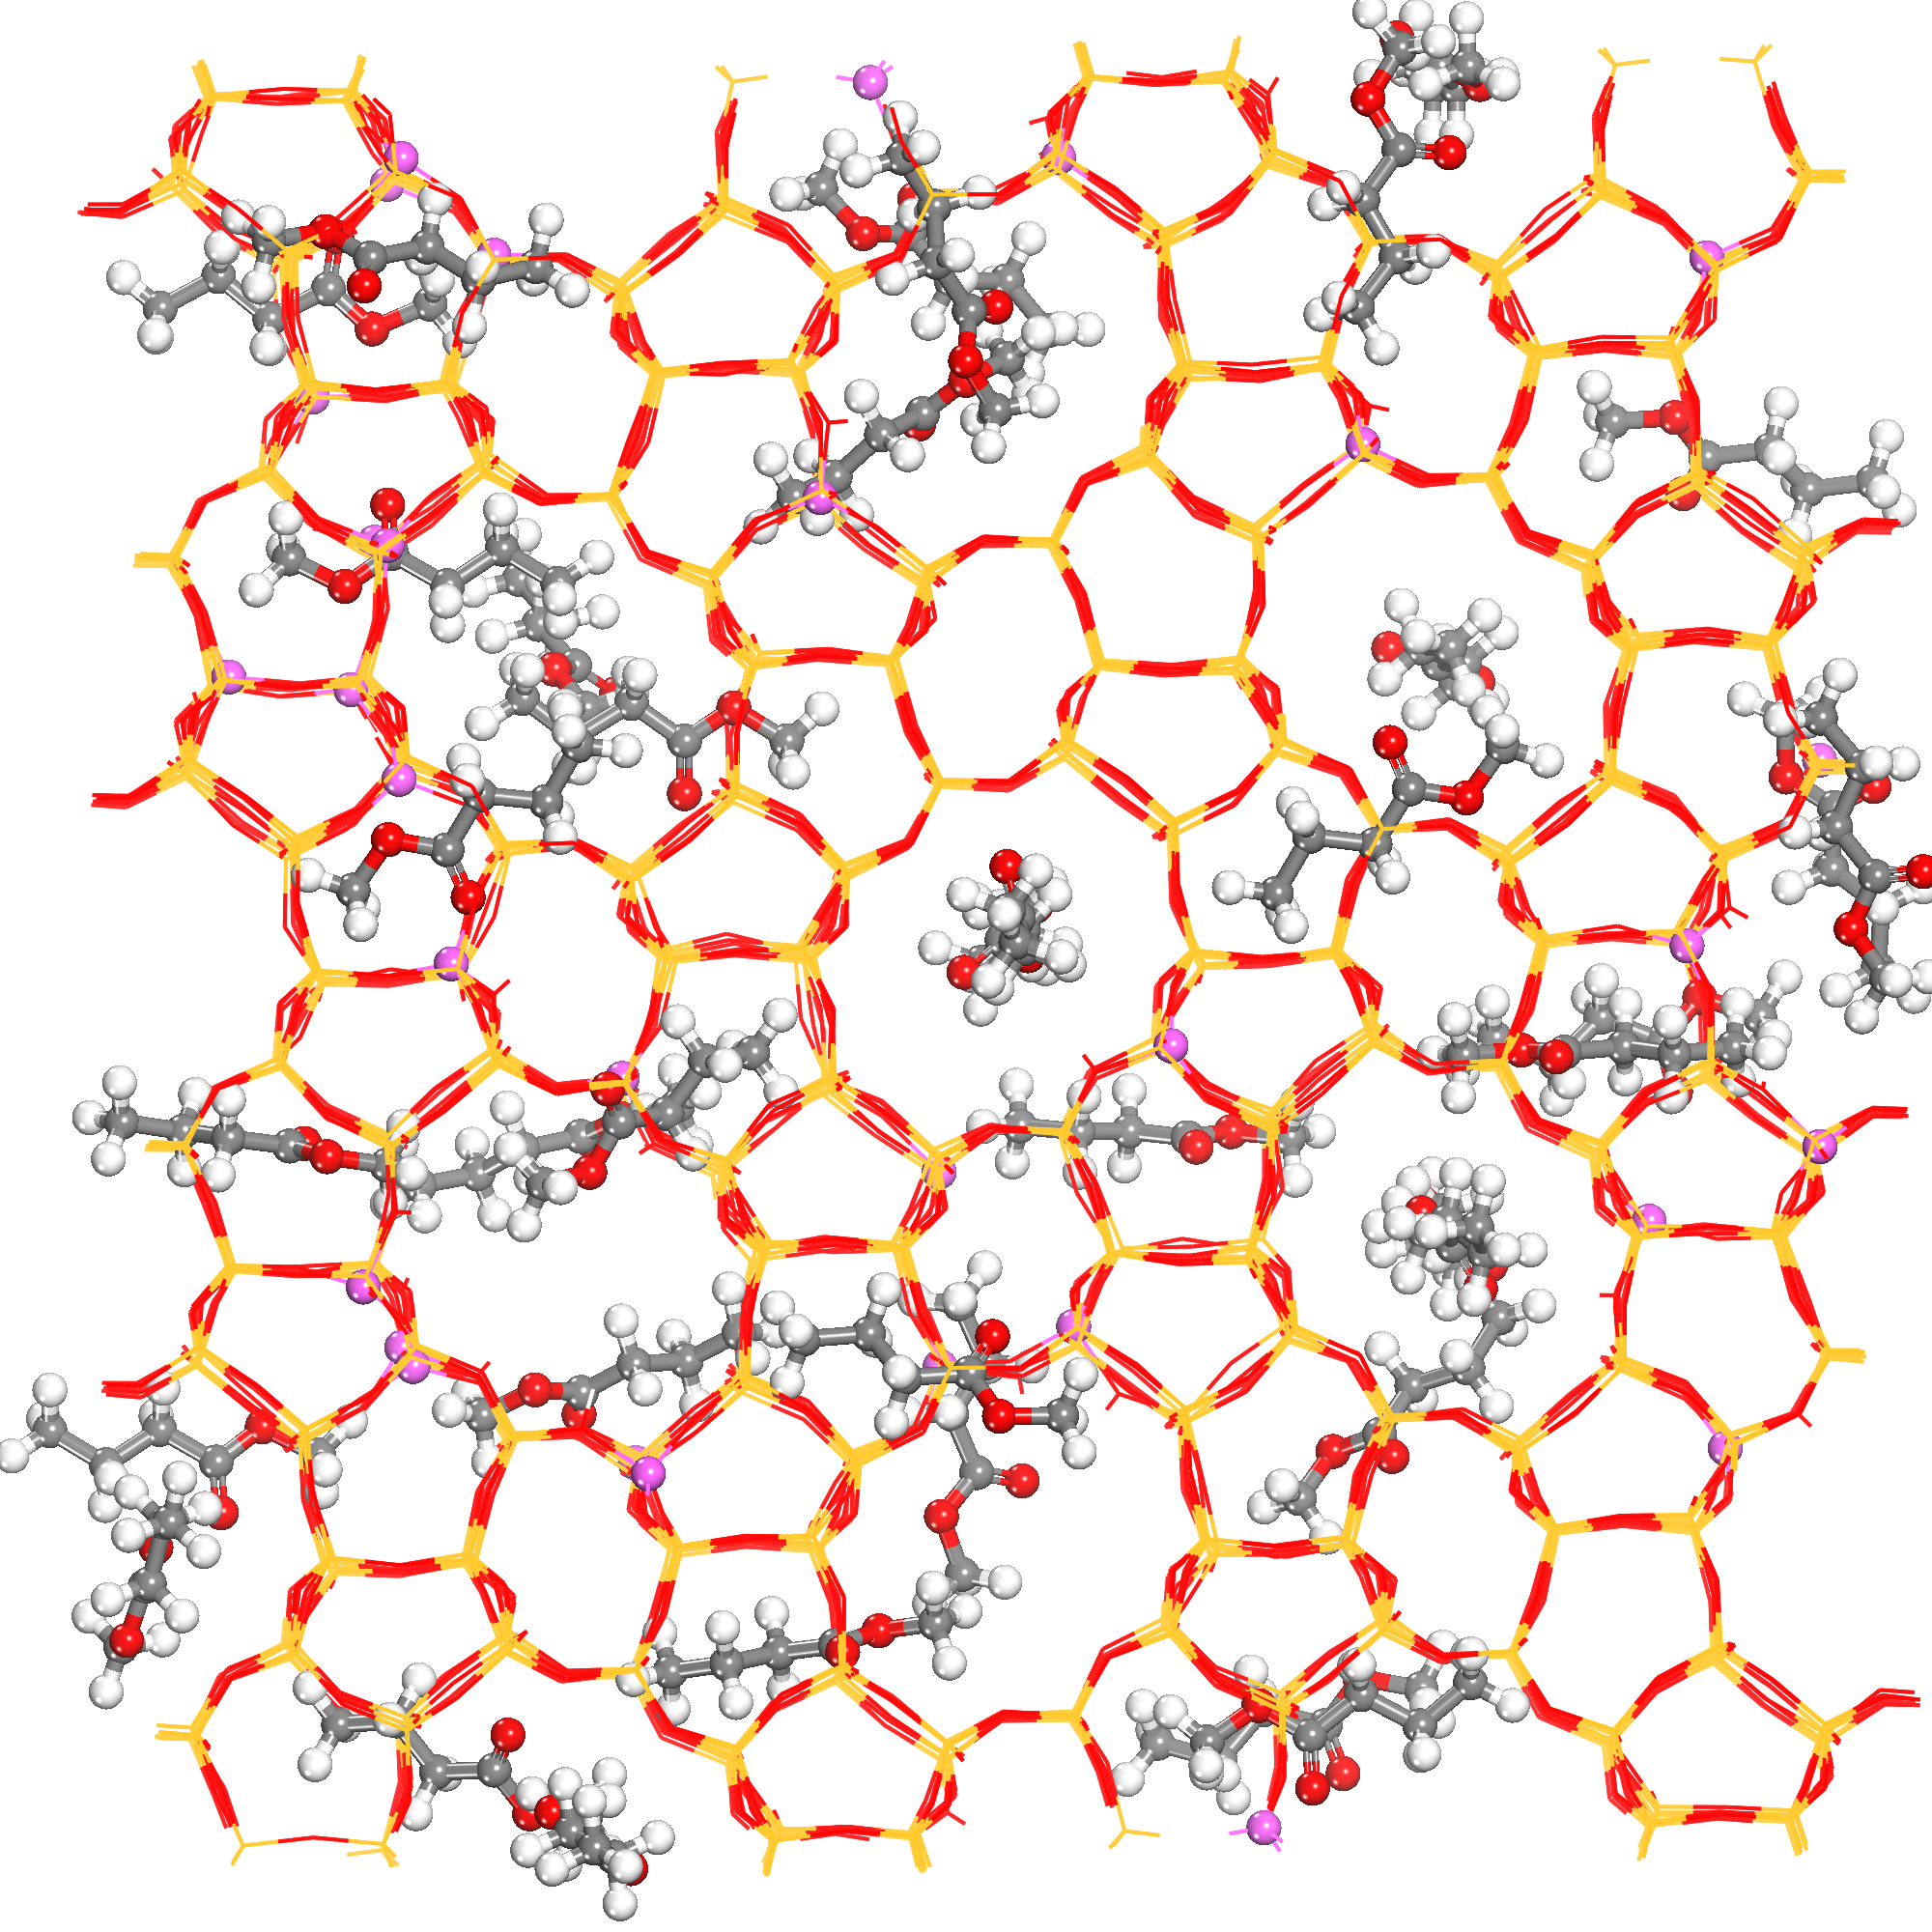
\includegraphics[width=1.8in]{figure/Adsorption/lowB.png}
    %\caption{fig2}
    \end{minipage}%
    }%
    \subfigure[低压C方向]{
    \begin{minipage}[t]{0.3333\linewidth}
    \centering
    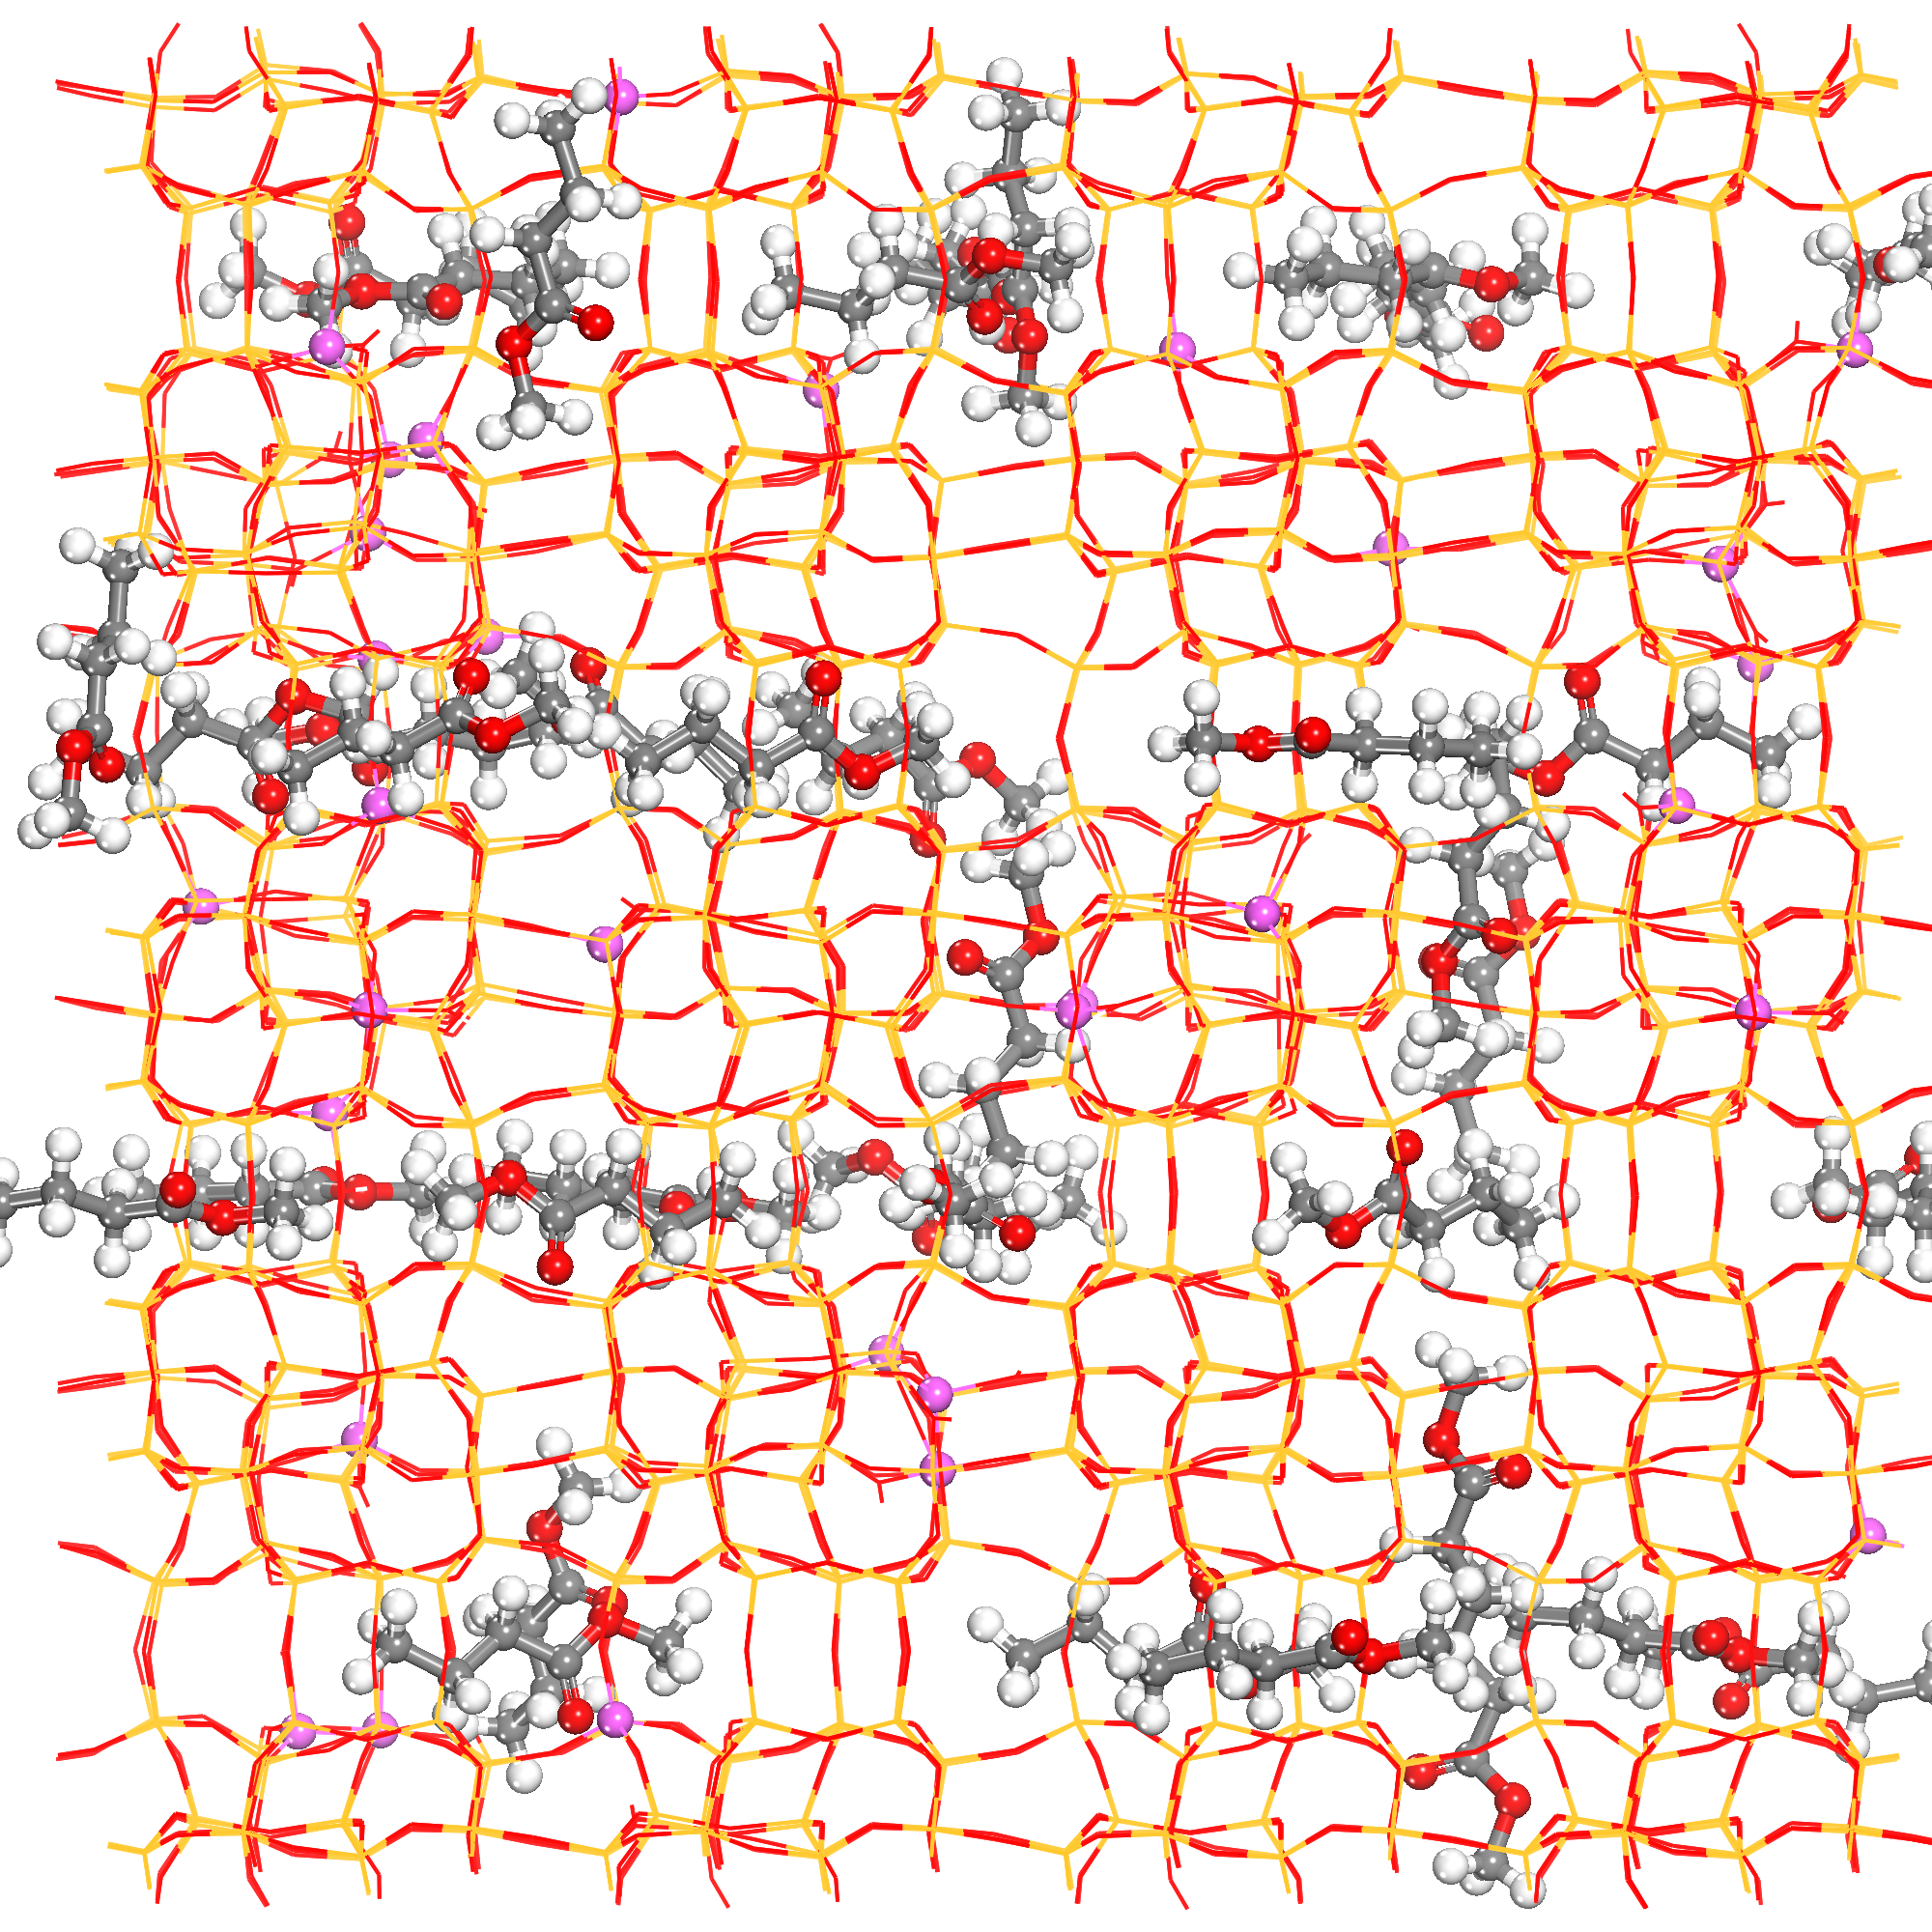
\includegraphics[width=1.8in]{figure/Adsorption/lowC.png}
    %\caption{fig2}
    \end{minipage}%
    }%

    \subfigure[高压A方向]{
    \begin{minipage}[t]{0.3333\linewidth}
    \centering
    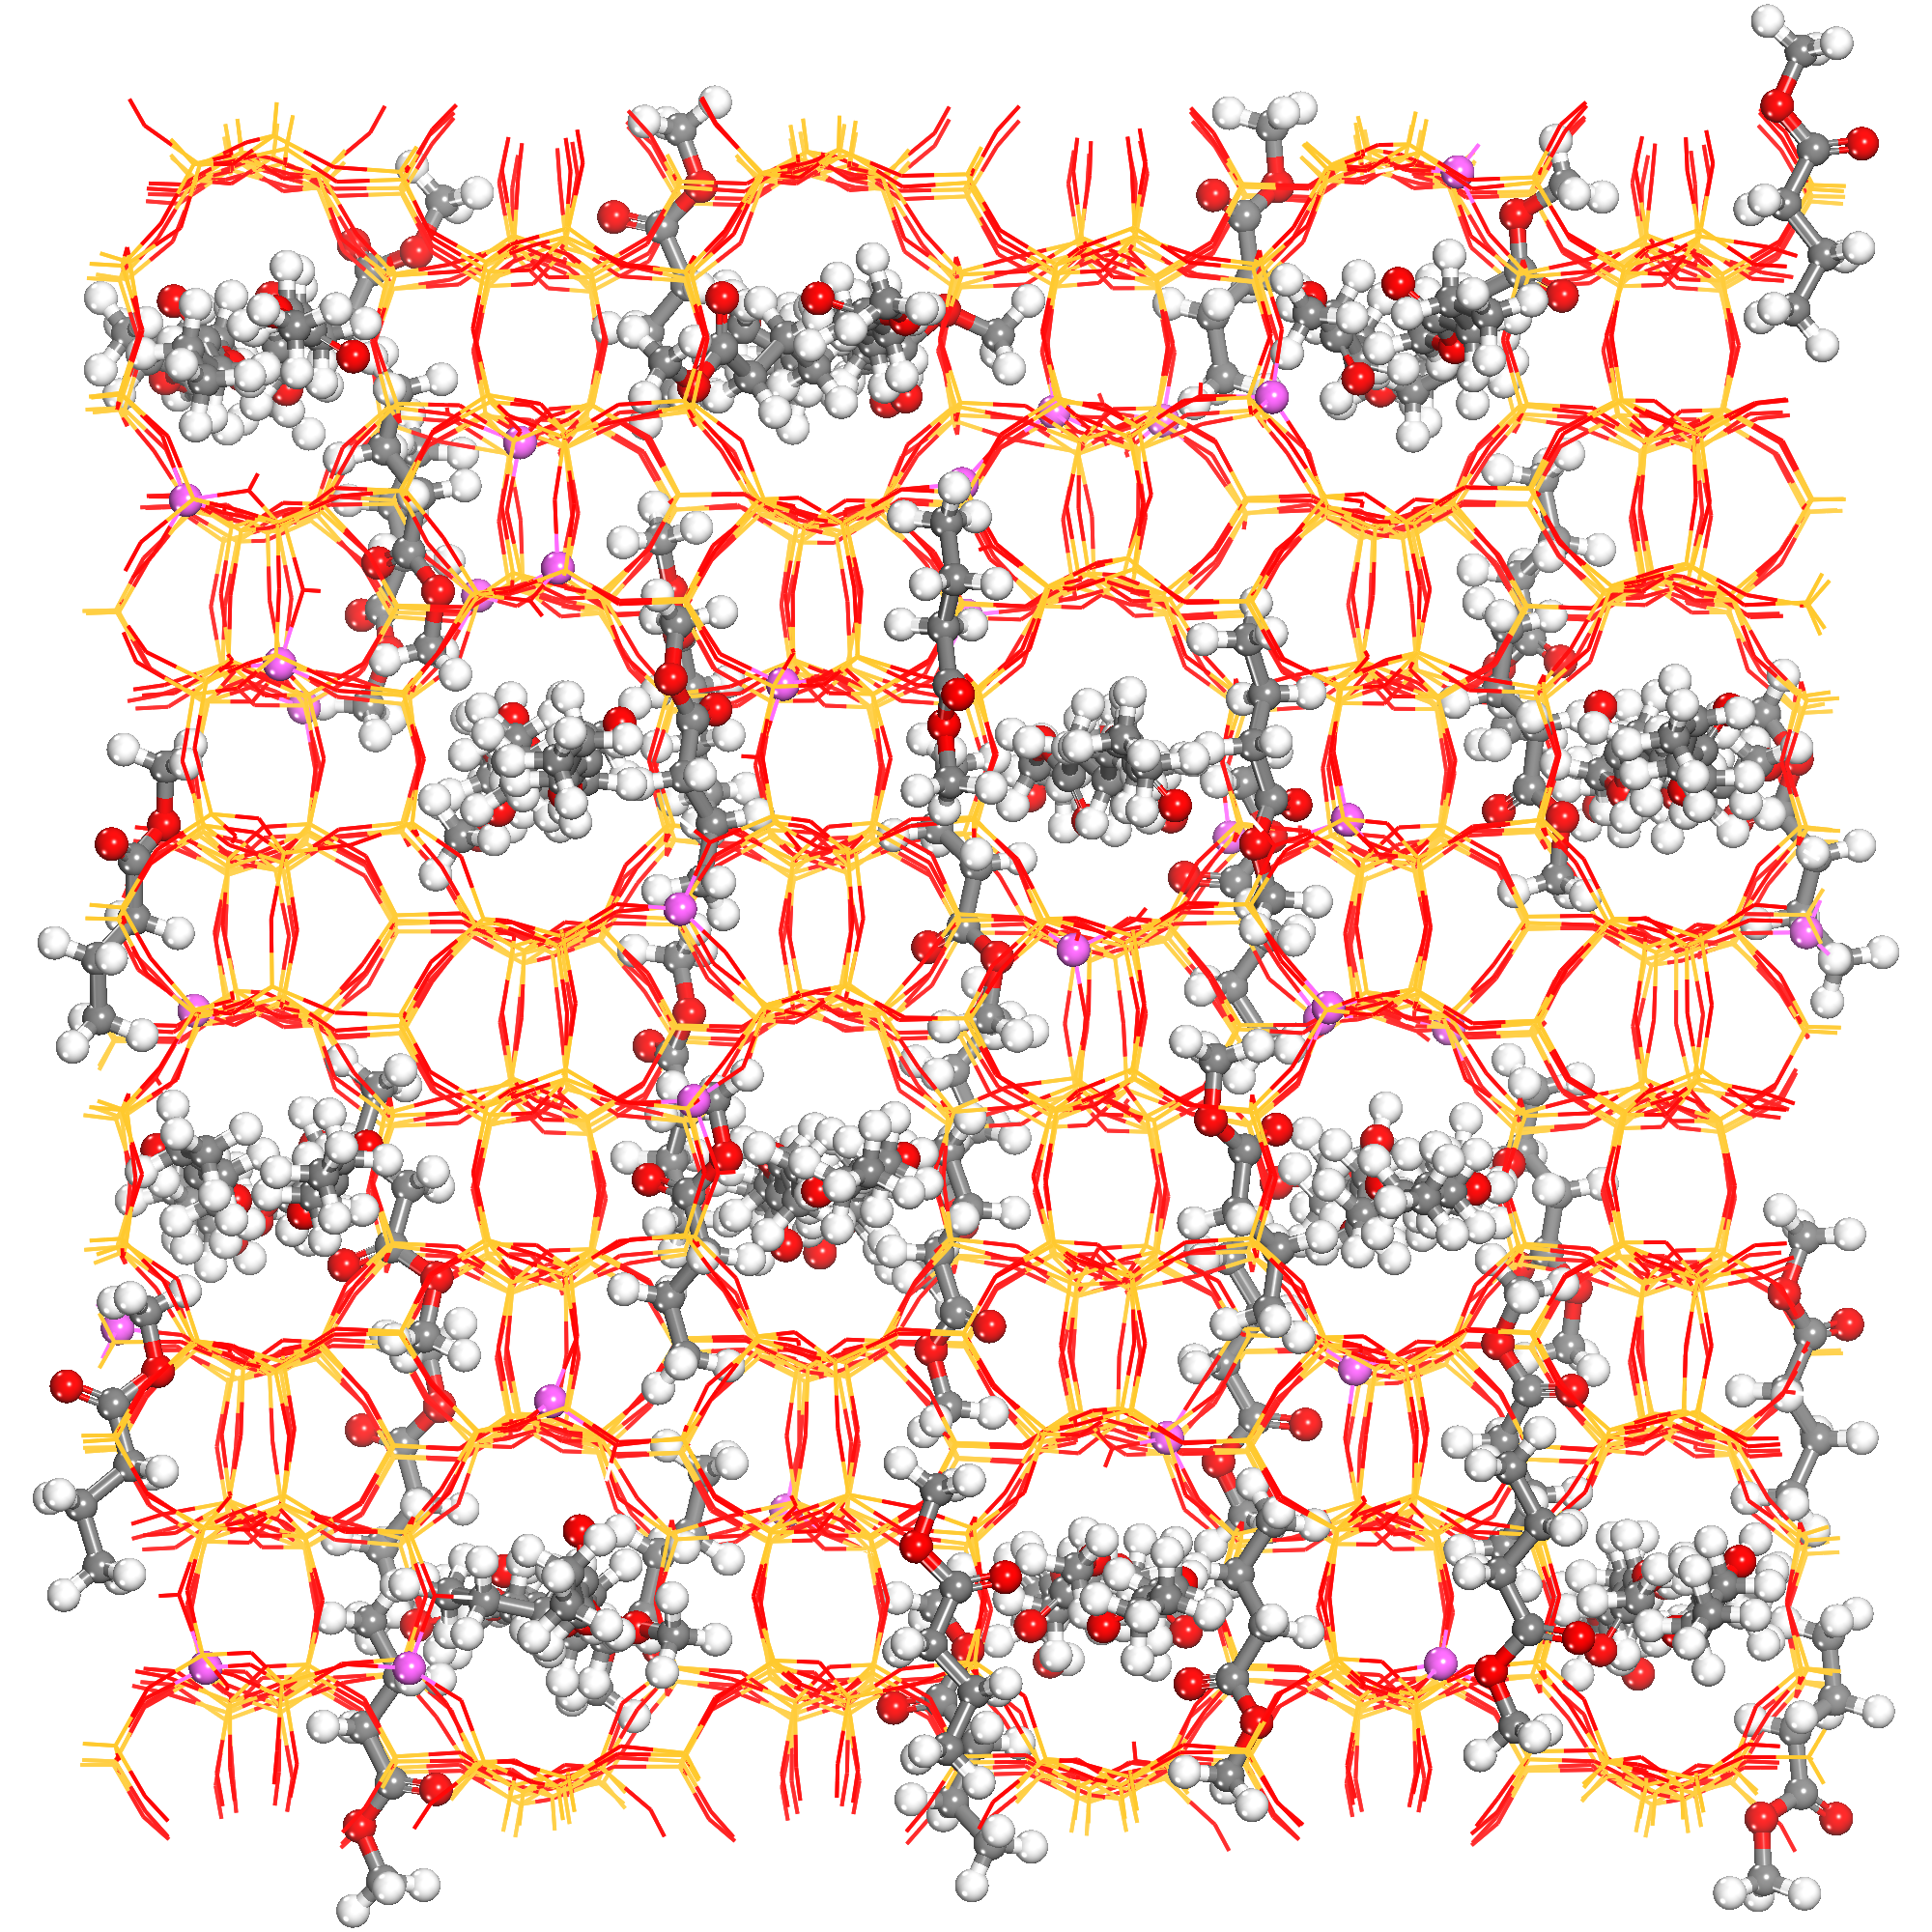
\includegraphics[width=1.8in]{figure/Adsorption/highA.png}
    %\caption{fig2}
    \end{minipage}%
    }%
    \subfigure[高压B方向]{
    \begin{minipage}[t]{0.3333\linewidth}
    \centering
    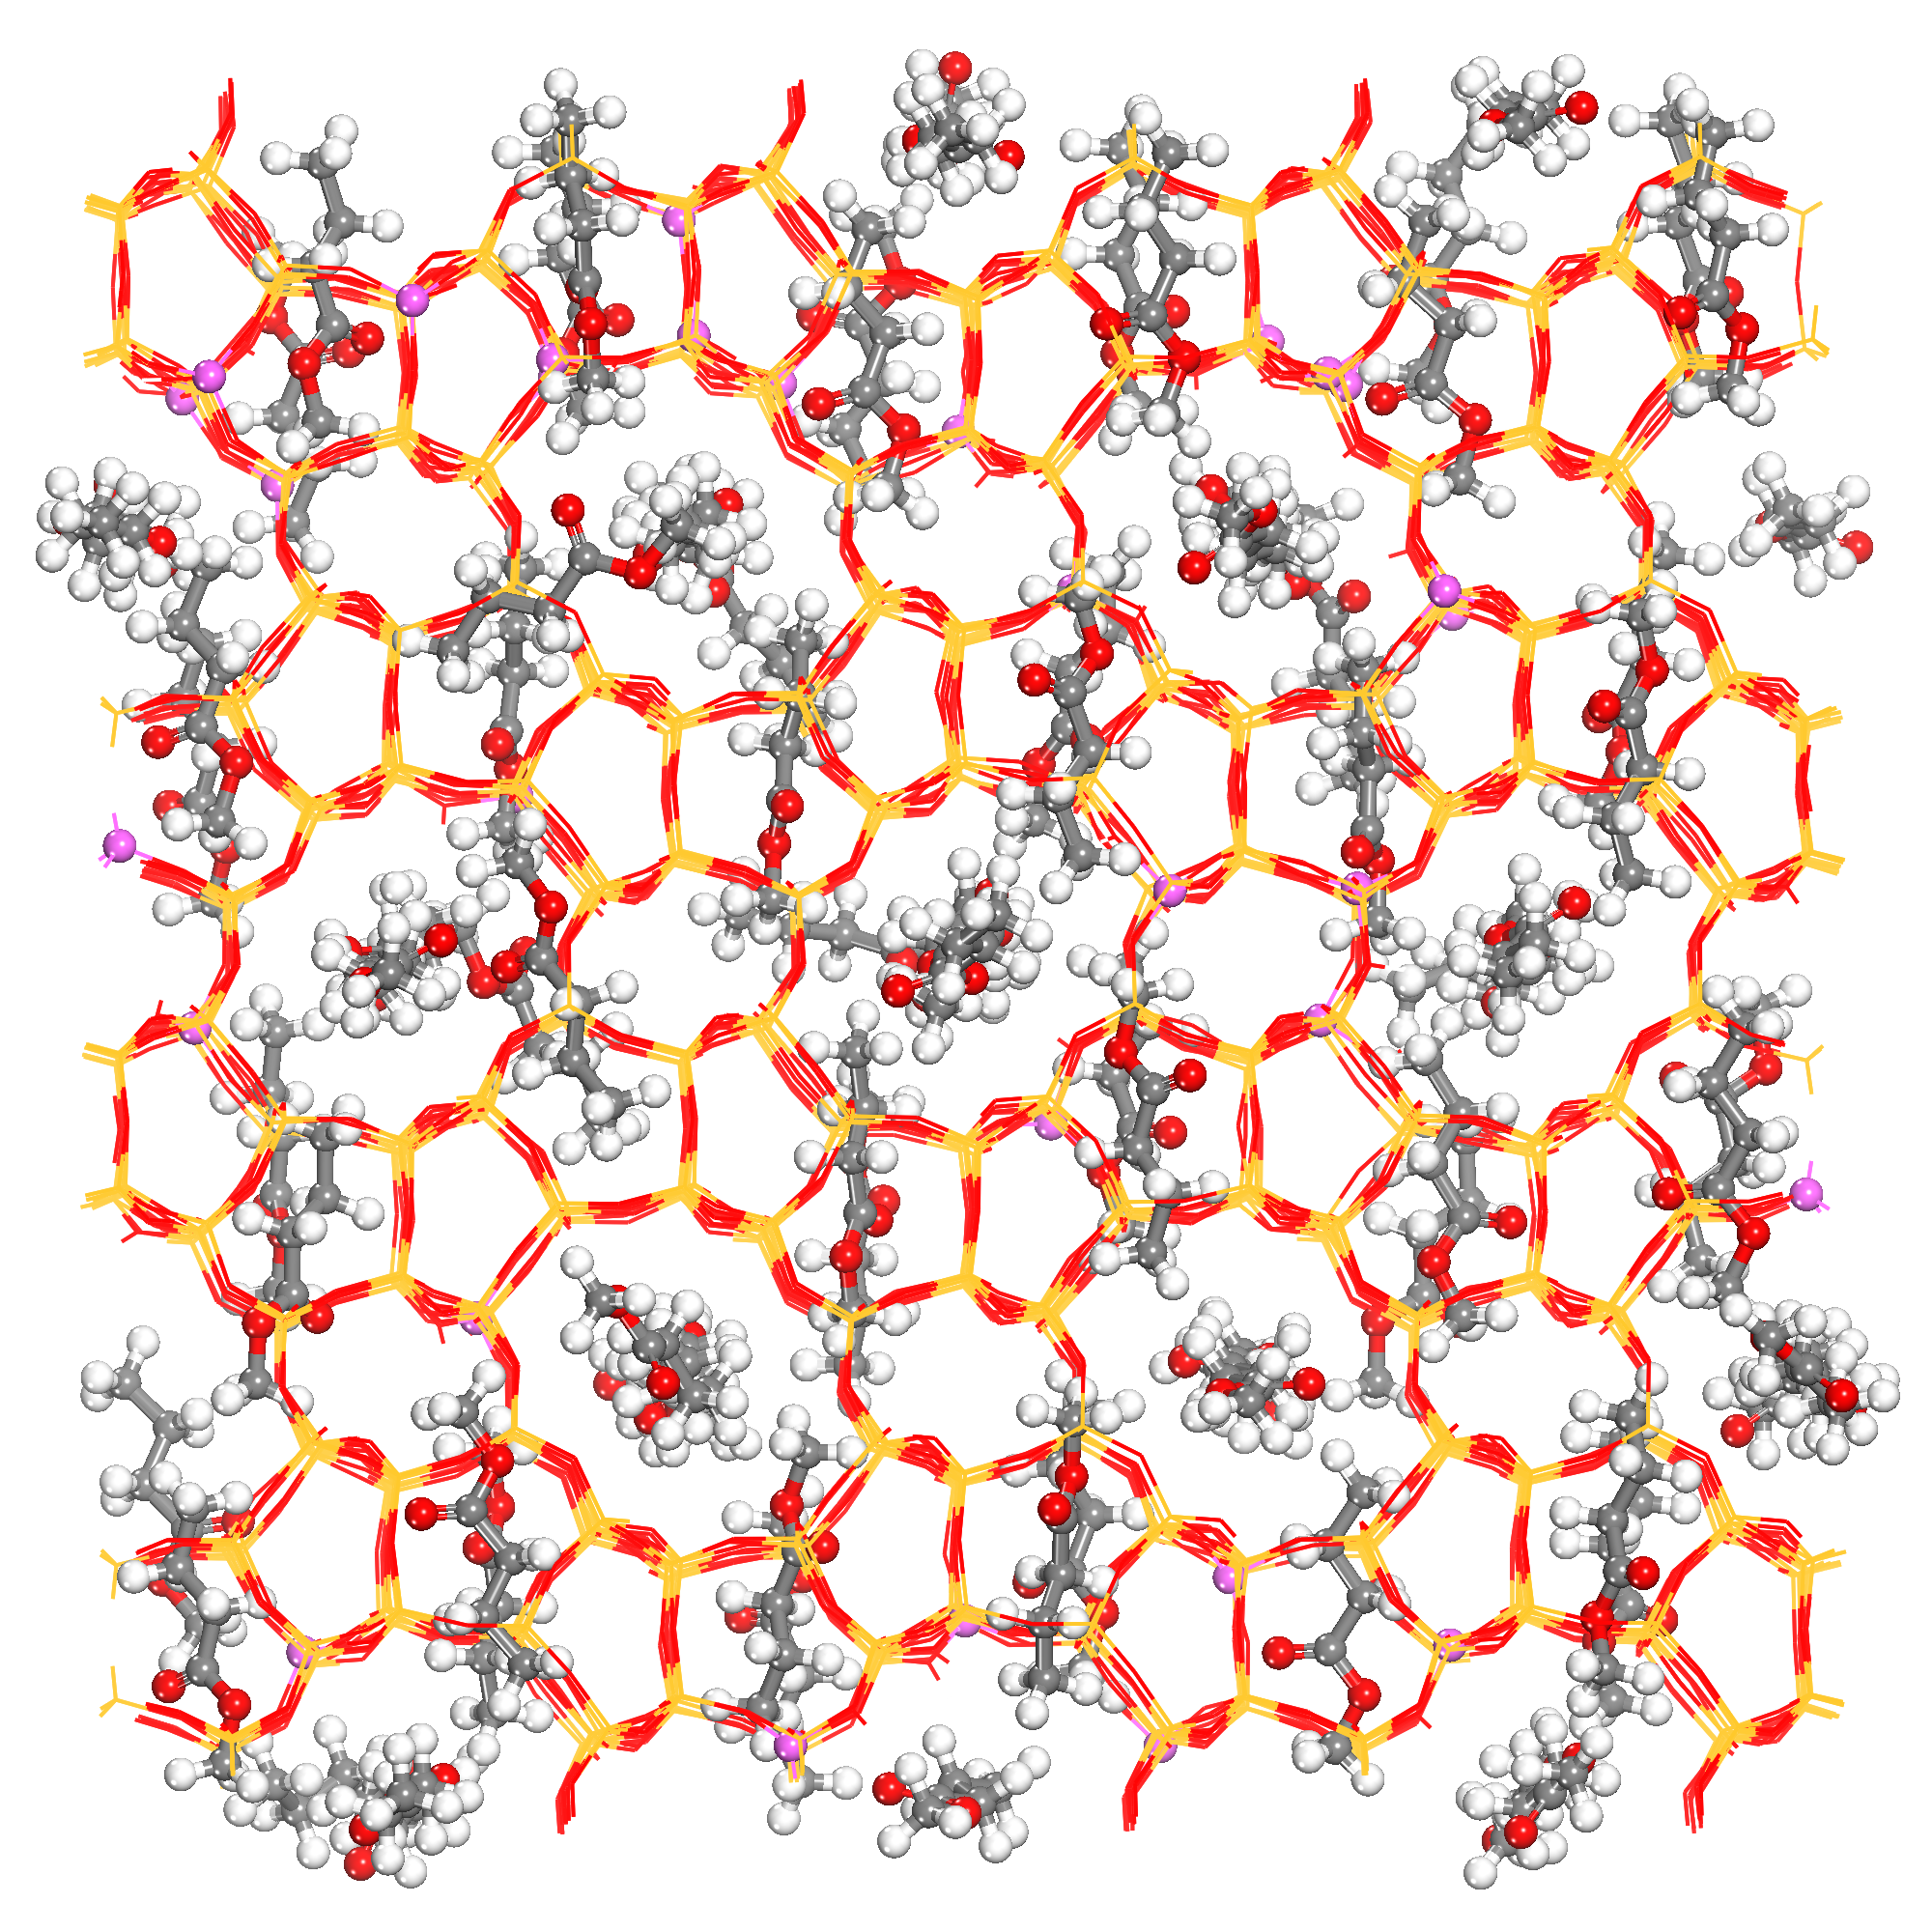
\includegraphics[width=1.8in]{figure/Adsorption/highB.png}
    %\caption{fig2}
    \end{minipage}%
    }%
    \subfigure[高压C方向]{
    \begin{minipage}[t]{0.3333\linewidth}
    \centering
    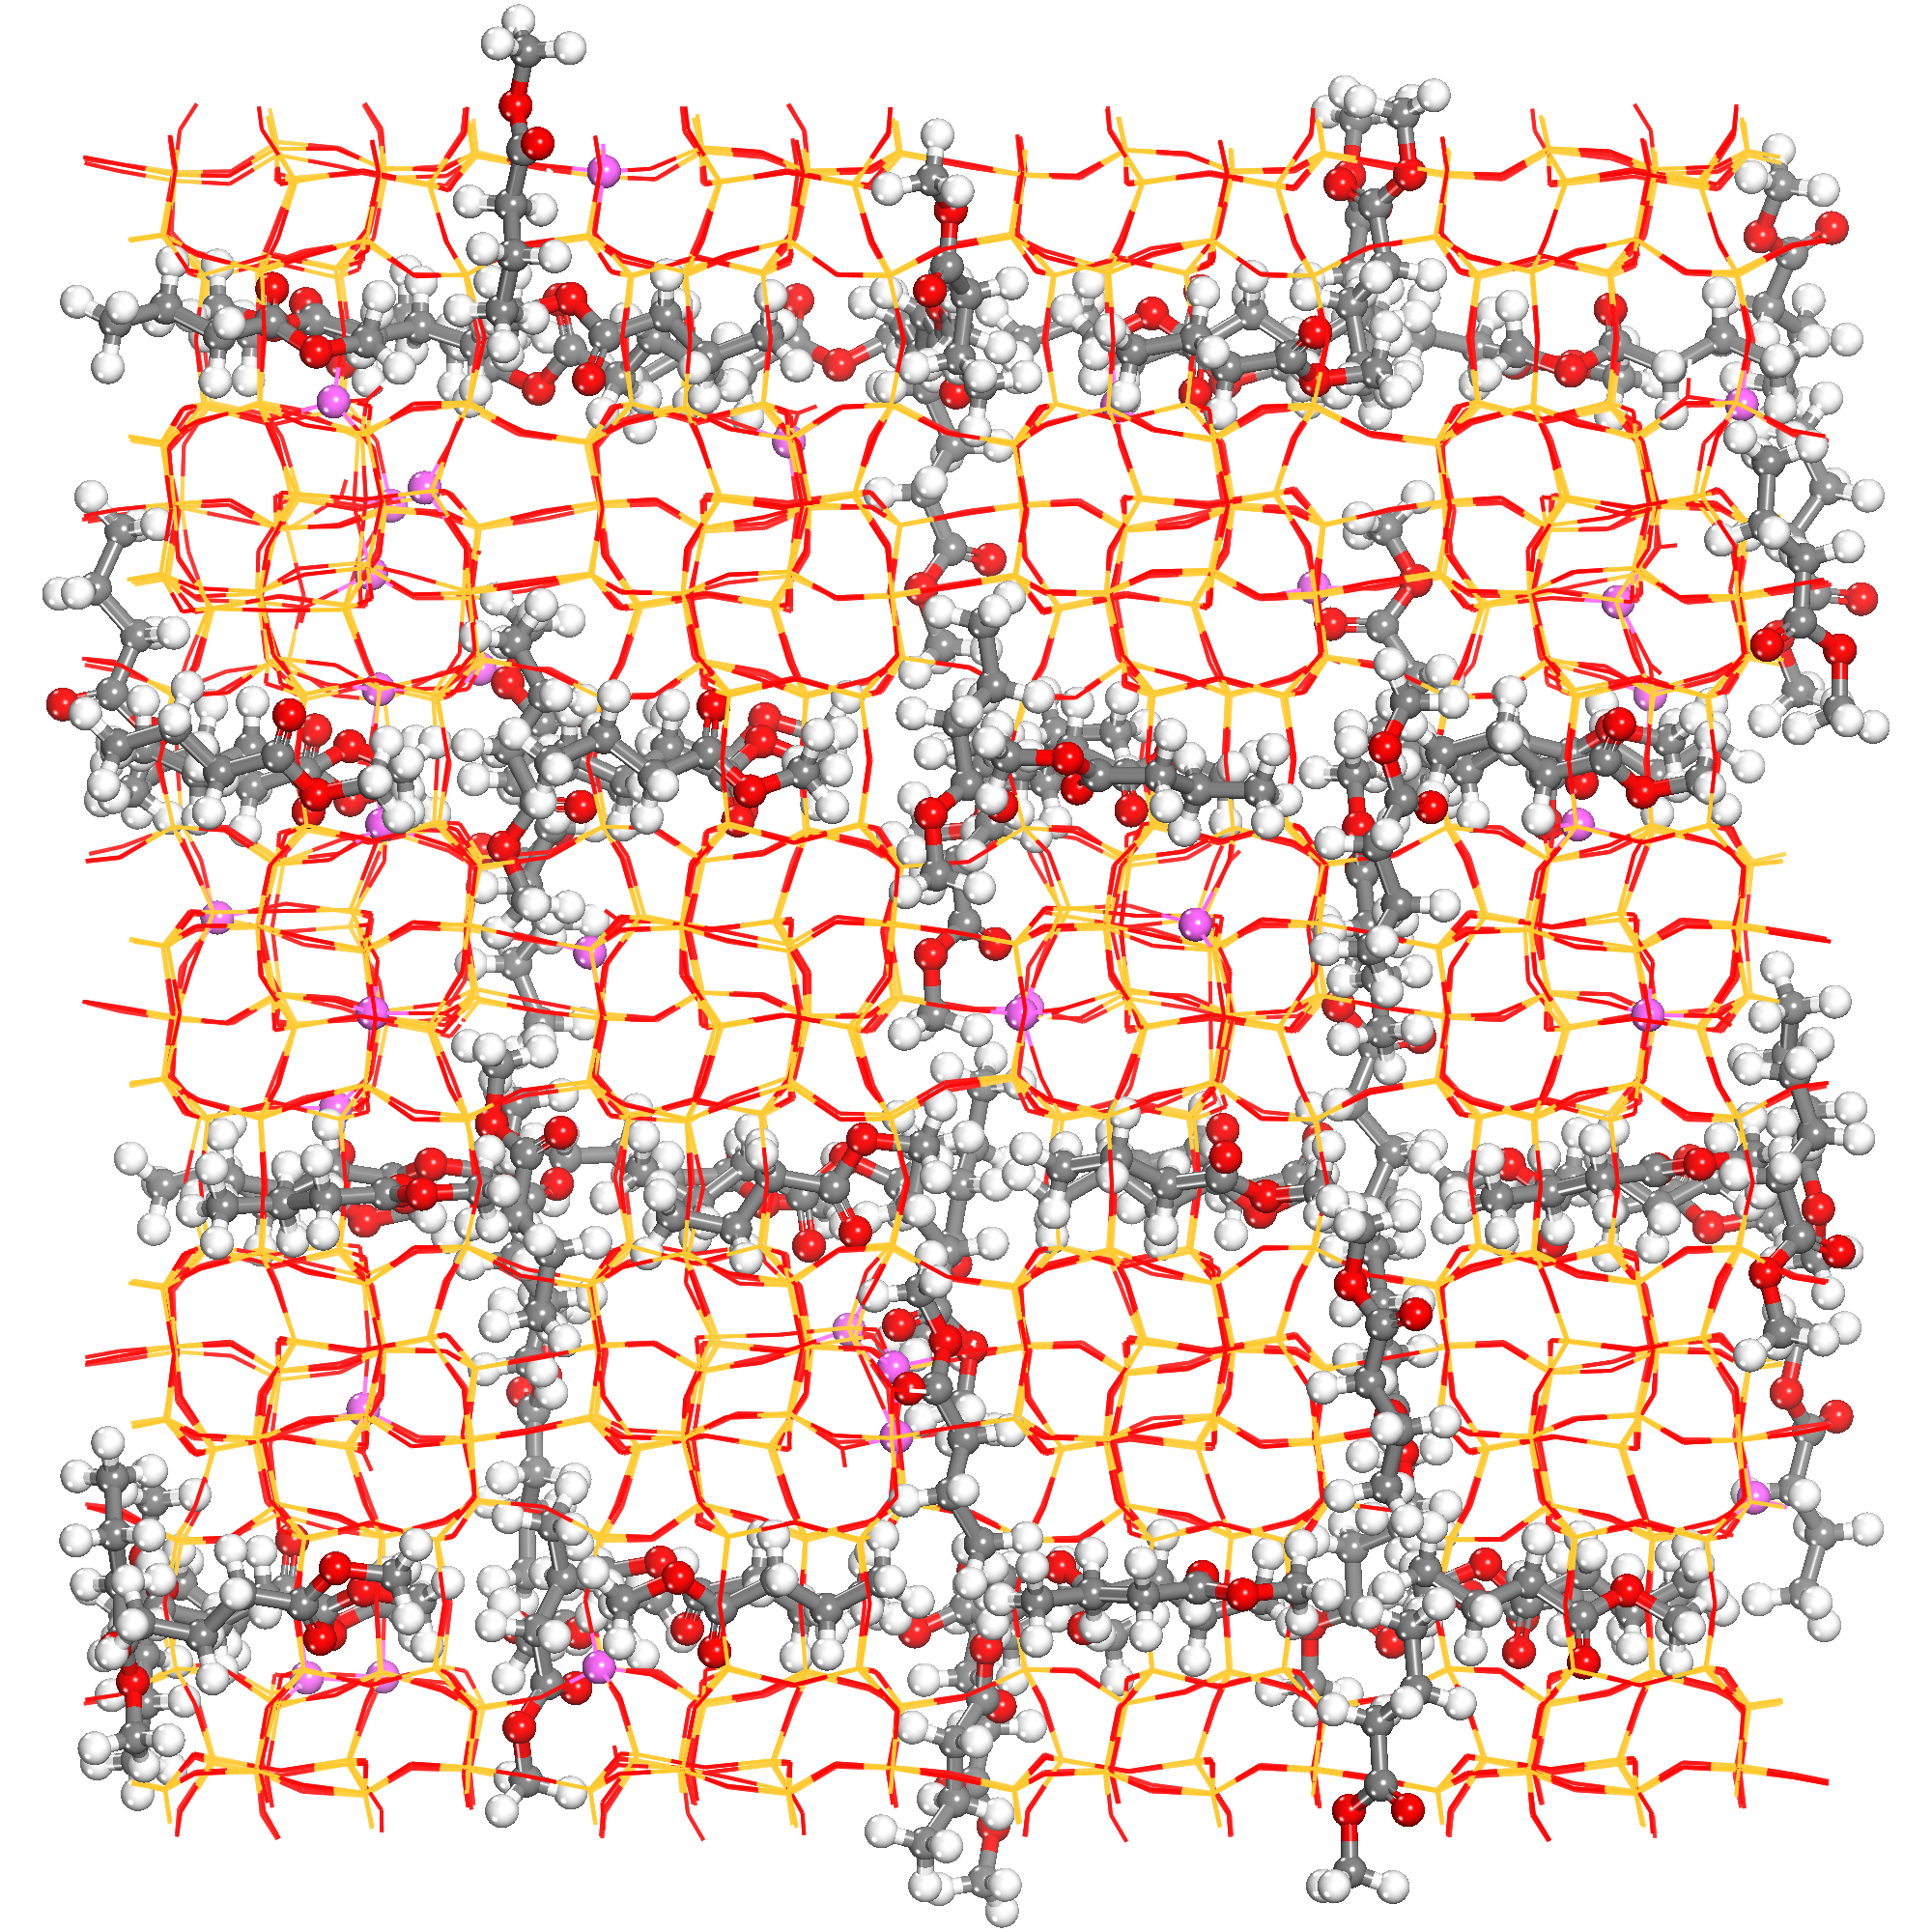
\includegraphics[width=1.8in]{figure/Adsorption/highC.png}
    %\caption{fig2}
    \end{minipage}%
    }%
    \caption{高低压力对丁酸甲酯吸附位置的构型对比图}
    \label{fig:loaction}
\end{figure}
\par{通过\reffig{fig:loaction}可以看出丁酸甲酯优先吸附在活性吸附位(B 位酸)处,并分布在交叉孔道旁,随着压力的增大,丁酸甲酯在交叉孔道和直孔道都有吸附,这与上文的结论是一致的,先吸附活性吸附位,再吸附一般吸附位。而通过\reffig{fig:L1}可以清楚地看到,丁酸甲酯中的双键氧与分子筛上的桥键氧上的氢(B位酸)形成了氢键。因为氢键的作用力比范德华力大,所以丁酸甲酯附着在活性吸附位放出的热量比一般吸附位大。从\reffig{fig:L2}可以看出,丁烯酸甲酯的双键与分子筛的B酸位相互作用形成 π 配位超分子复合物\cite{C-2-C-5直链烯烃在HY和H-ZSM-5分子筛上的吸附},使得丁烯酸甲酯与分子筛之间的作用力变强,从而丁烯酸甲酯的饱和吸附量更大,吸附平衡常数更大,这与上文的结论一致。}
% \begin{figure}[H]
%     \centering
%         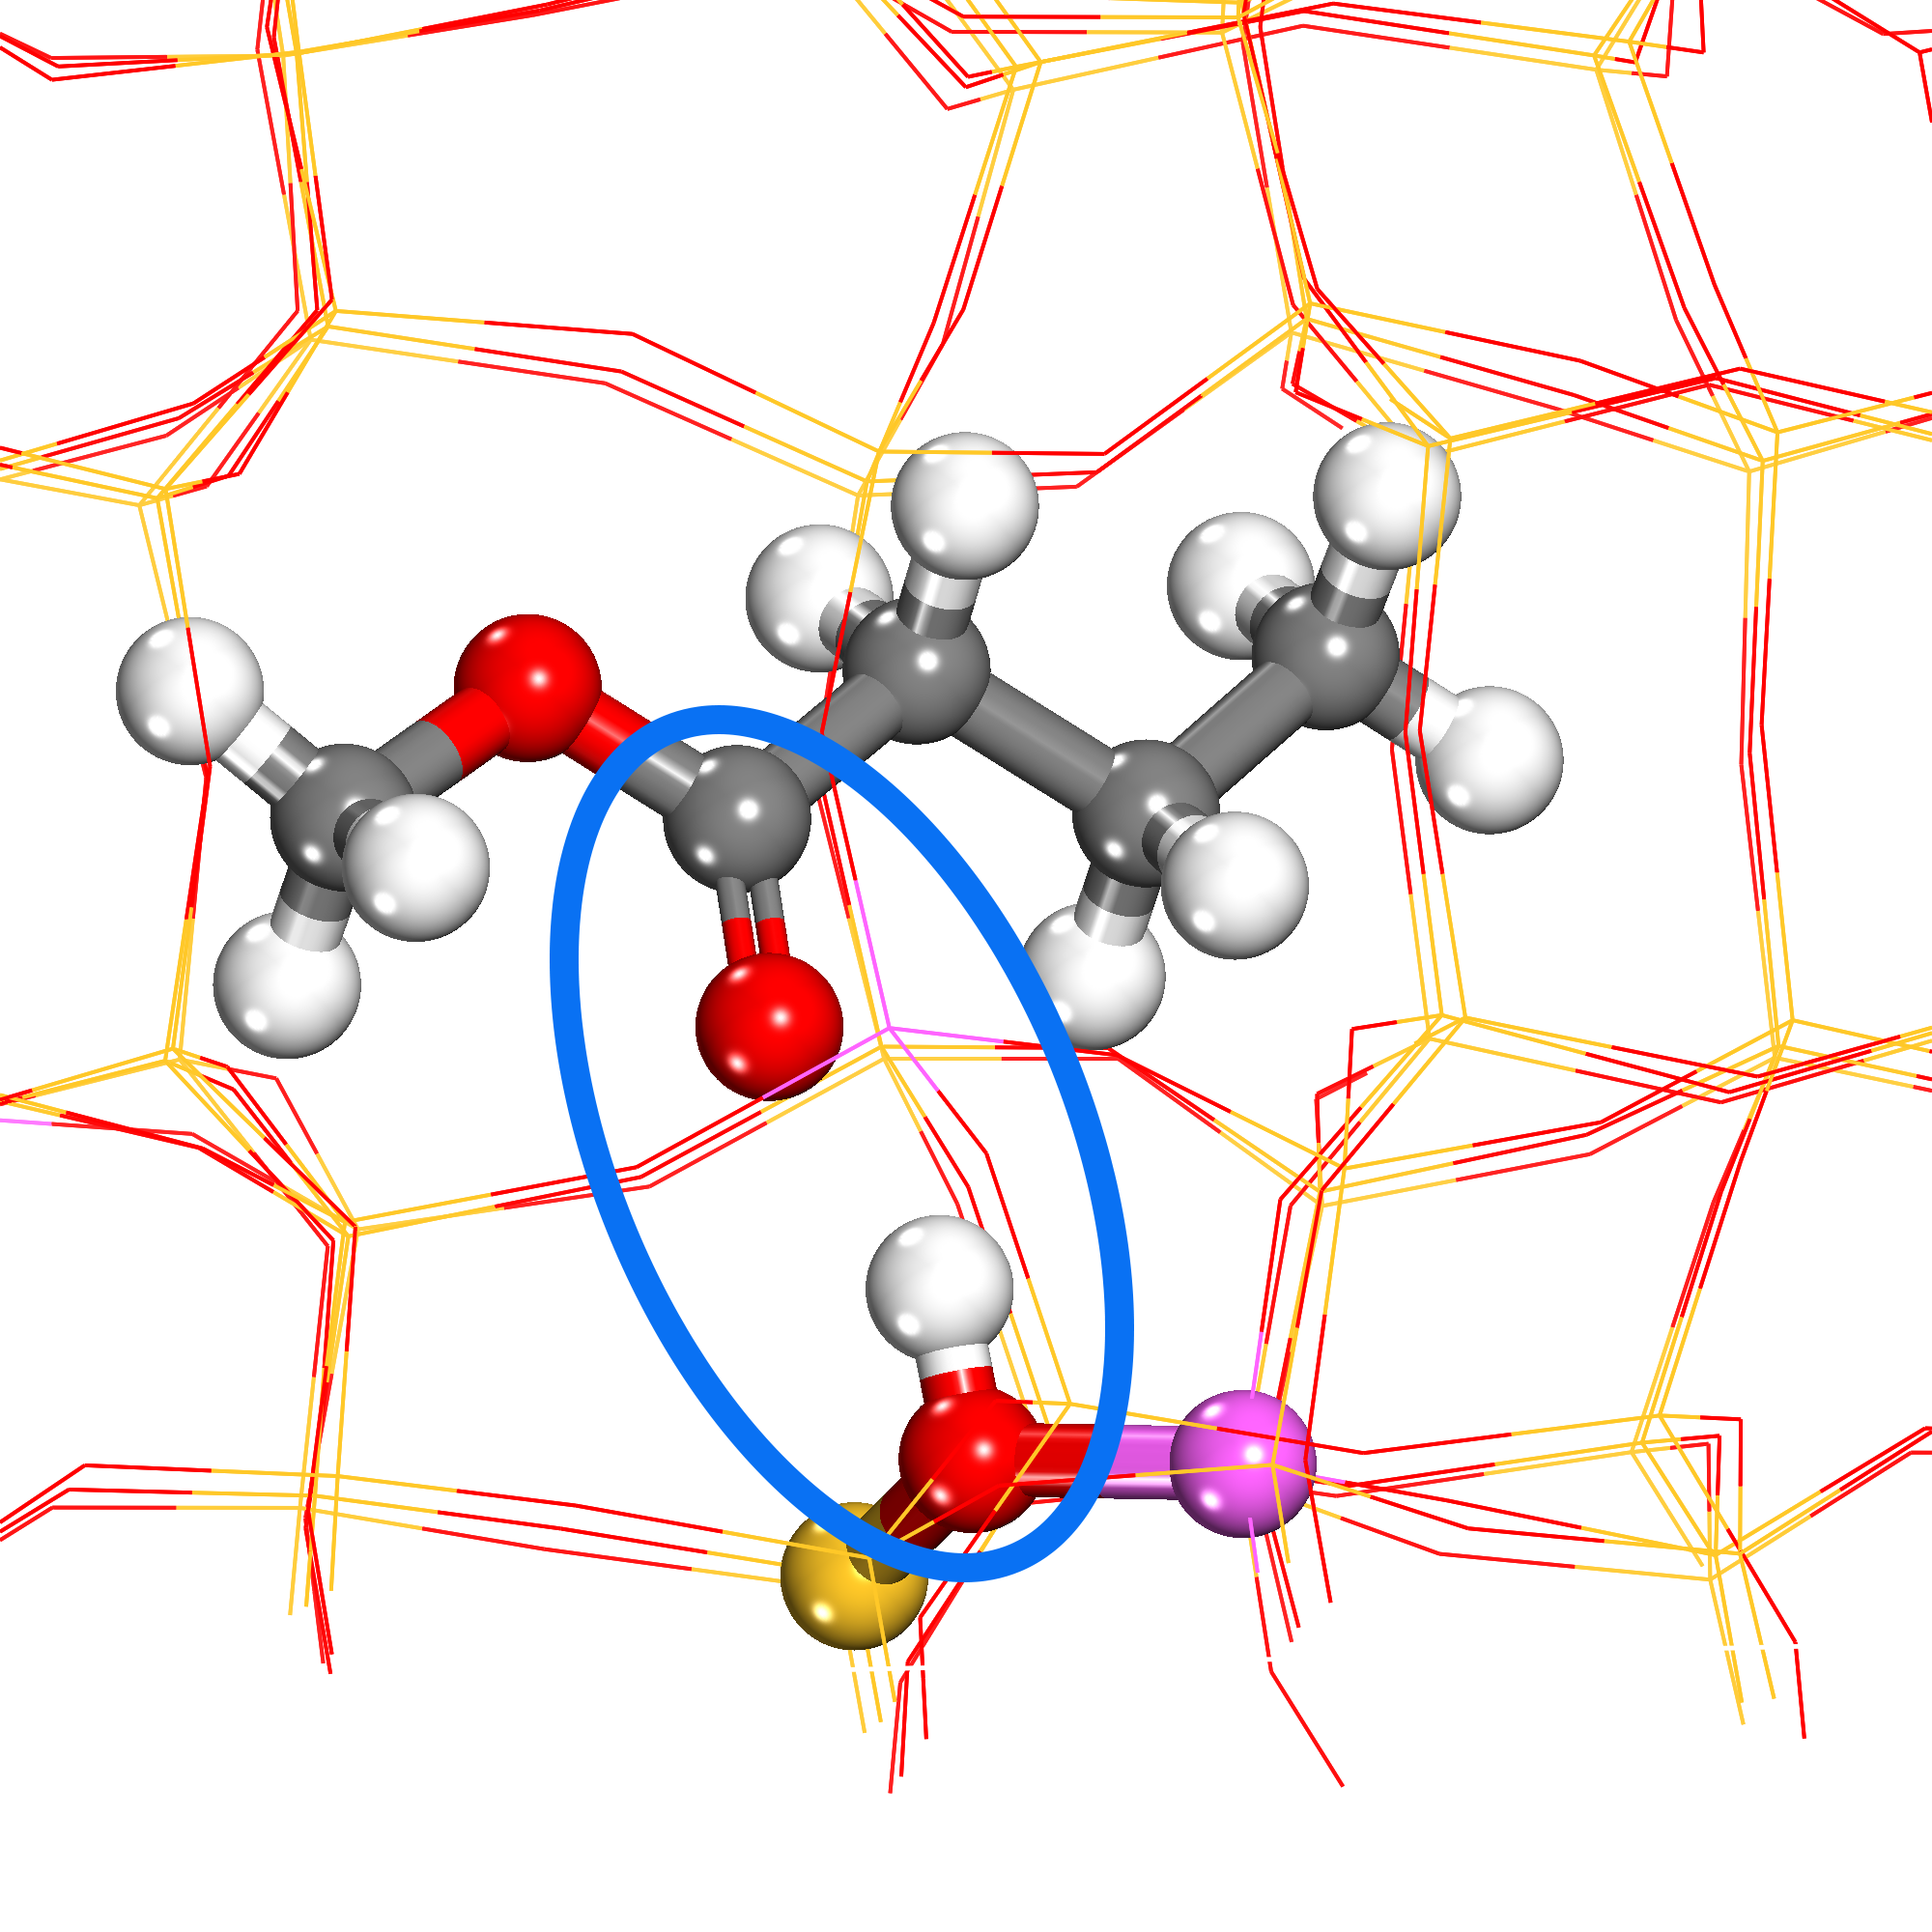
\includegraphics[width=0.5\textwidth]{figure/Adsorption/loaction.png}
%     \caption{丁酸甲酯与B位酸吸附构型图}
%     \label{fig:L}
% \end{figure}
% \par{为了讨论双键对吸附位的影响,进行丁酸甲酯在H-ZSM-5分子筛中的吸附构型模拟,结果如\reffig{fig:L1}所示}

% \begin{figure}[H]
%     \centering
%         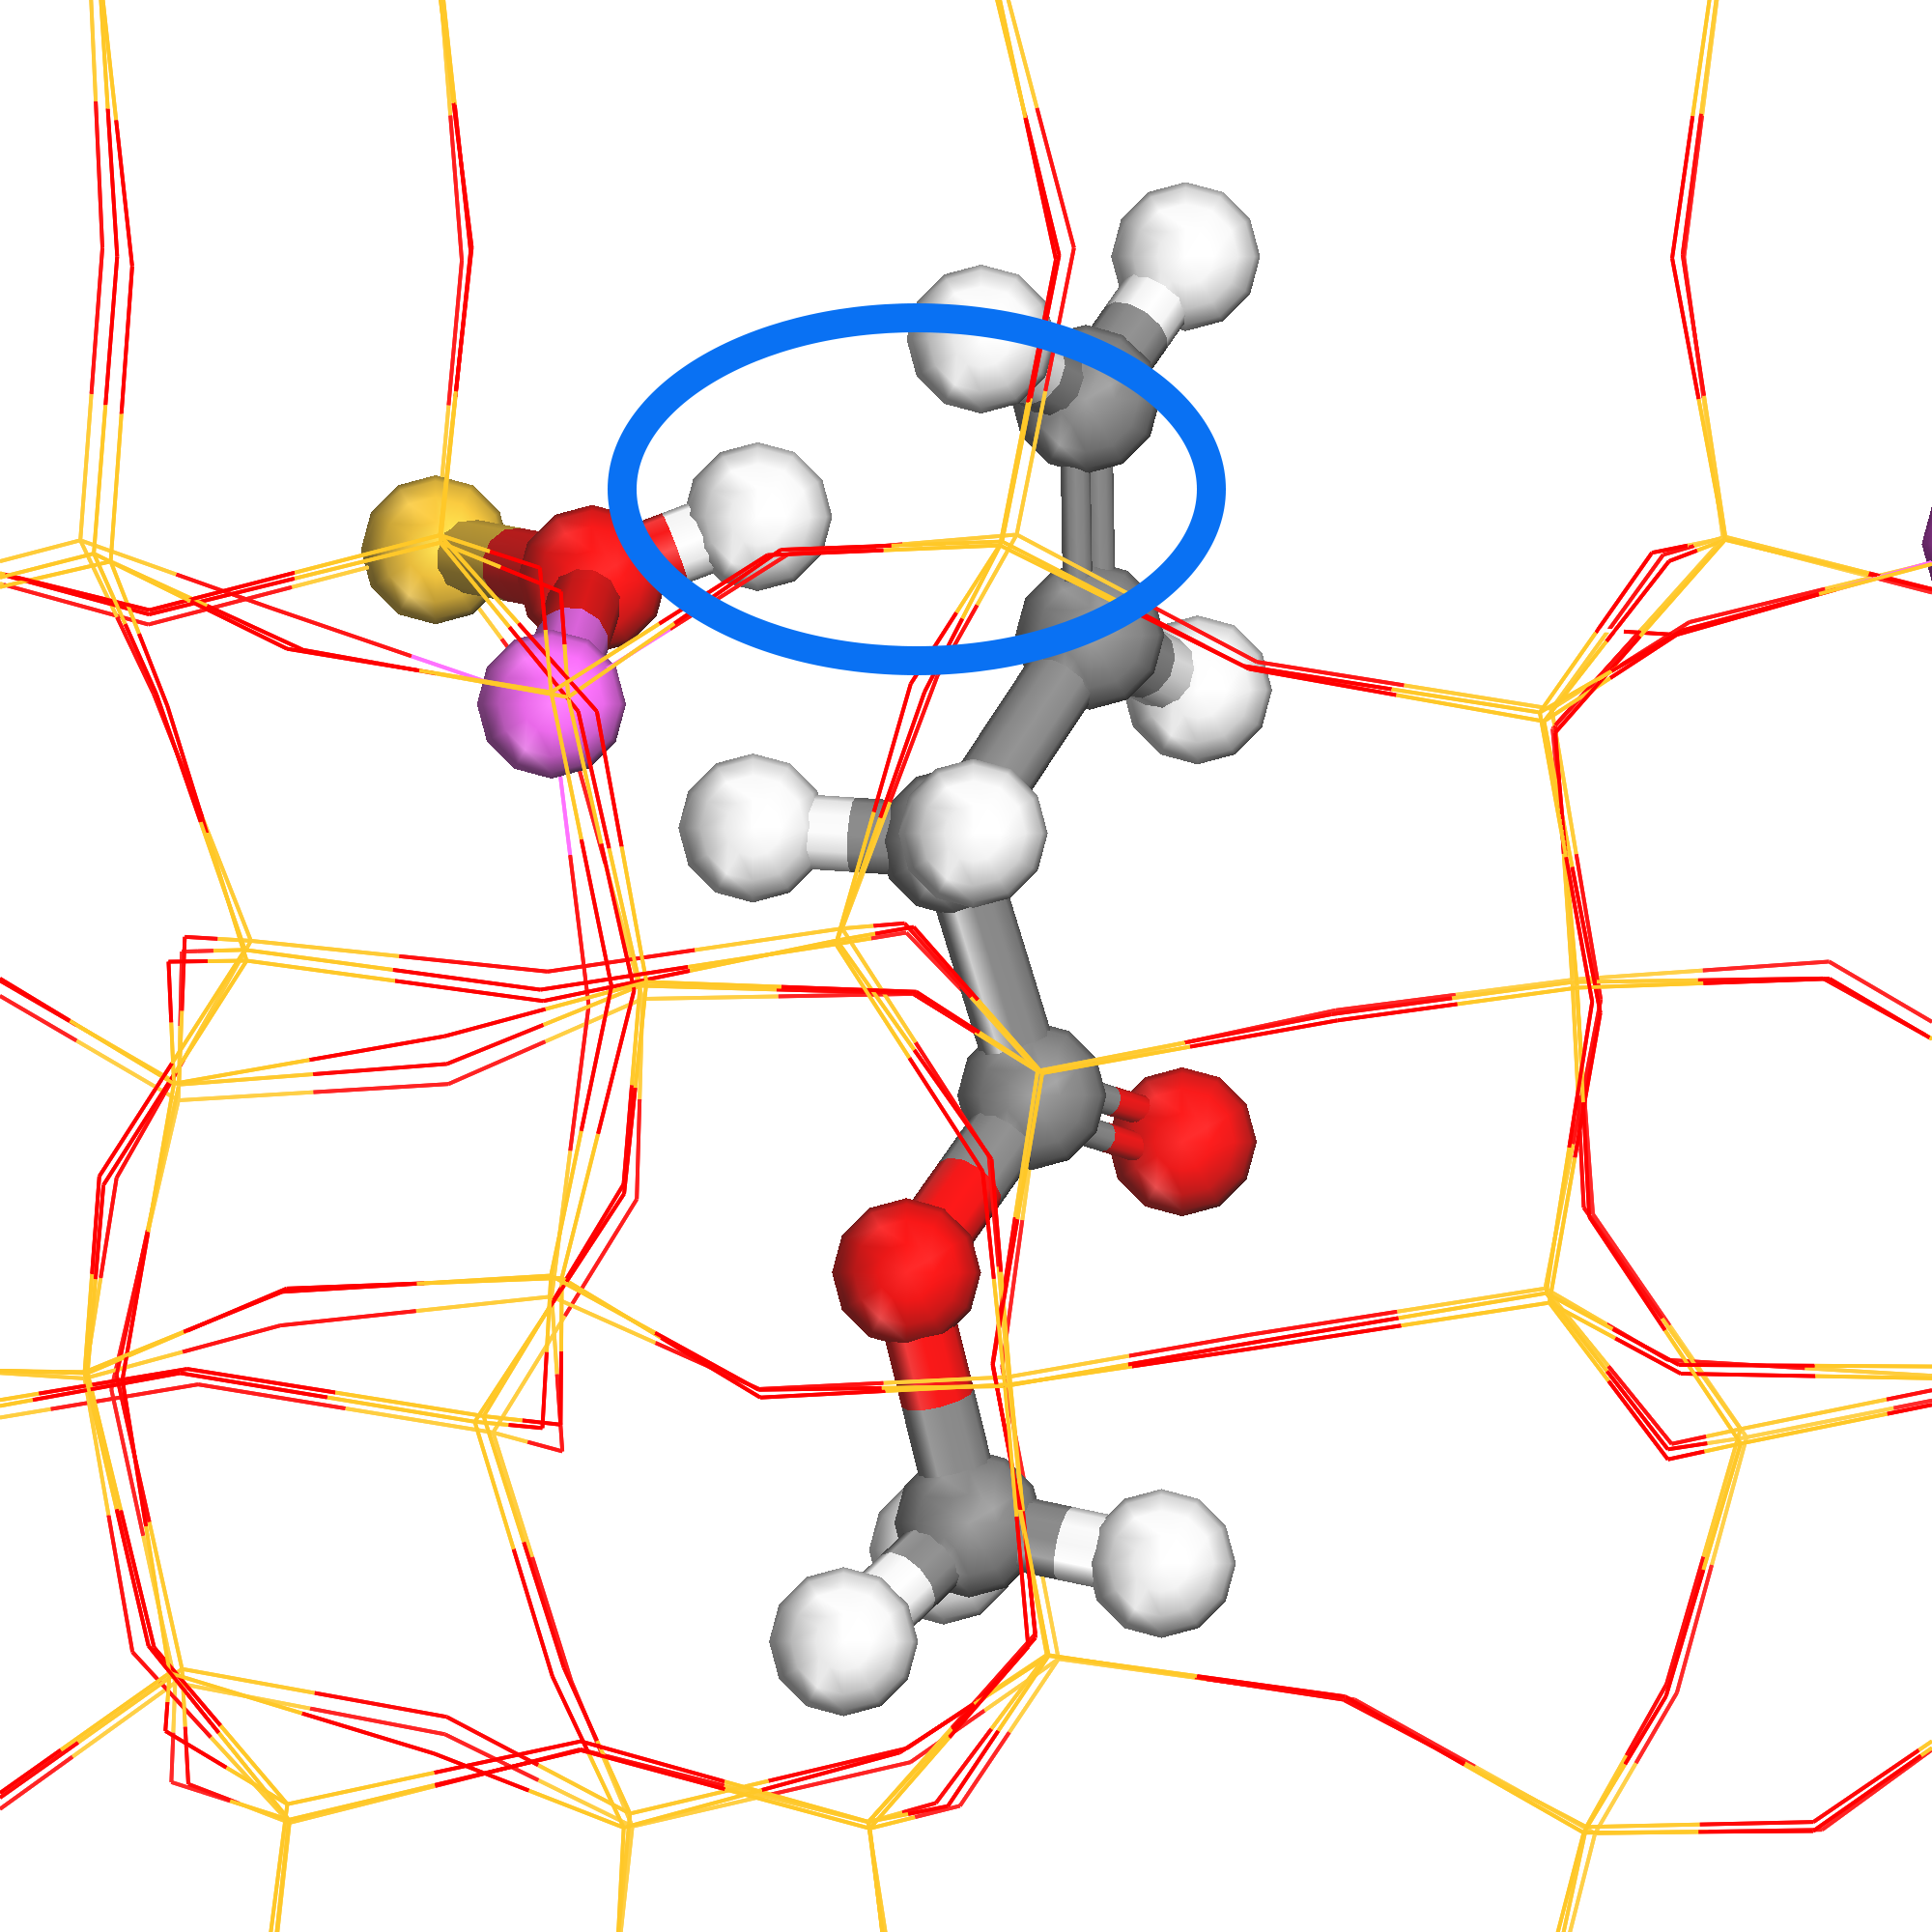
\includegraphics[width=0.5\textwidth]{figure/Adsorption/555.png}
%     \caption{丁烯酸甲酯与B位酸吸附构型图}
%     \label{fig:L1}
% \end{figure}
% \par{从\reffig{fig:L1}可以看出,丁烯酸甲酯的双键与分子筛的B酸位相互作用形成 π 配位超分子复合物\cite{C-2-C-5直链烯烃在HY和H-ZSM-5分子筛上的吸附},使得丁烯酸甲酯与分子筛之间的作用力变强,从而丁烯酸甲酯的饱和吸附量更大,吸附平衡常数更大,这与上文的结论一致。}

\begin{figure}[H]
    \centering

    \subfigure[丁酸甲酯与B位酸吸附构型图]{
    \begin{minipage}[t]{0.5\linewidth}
    \centering
    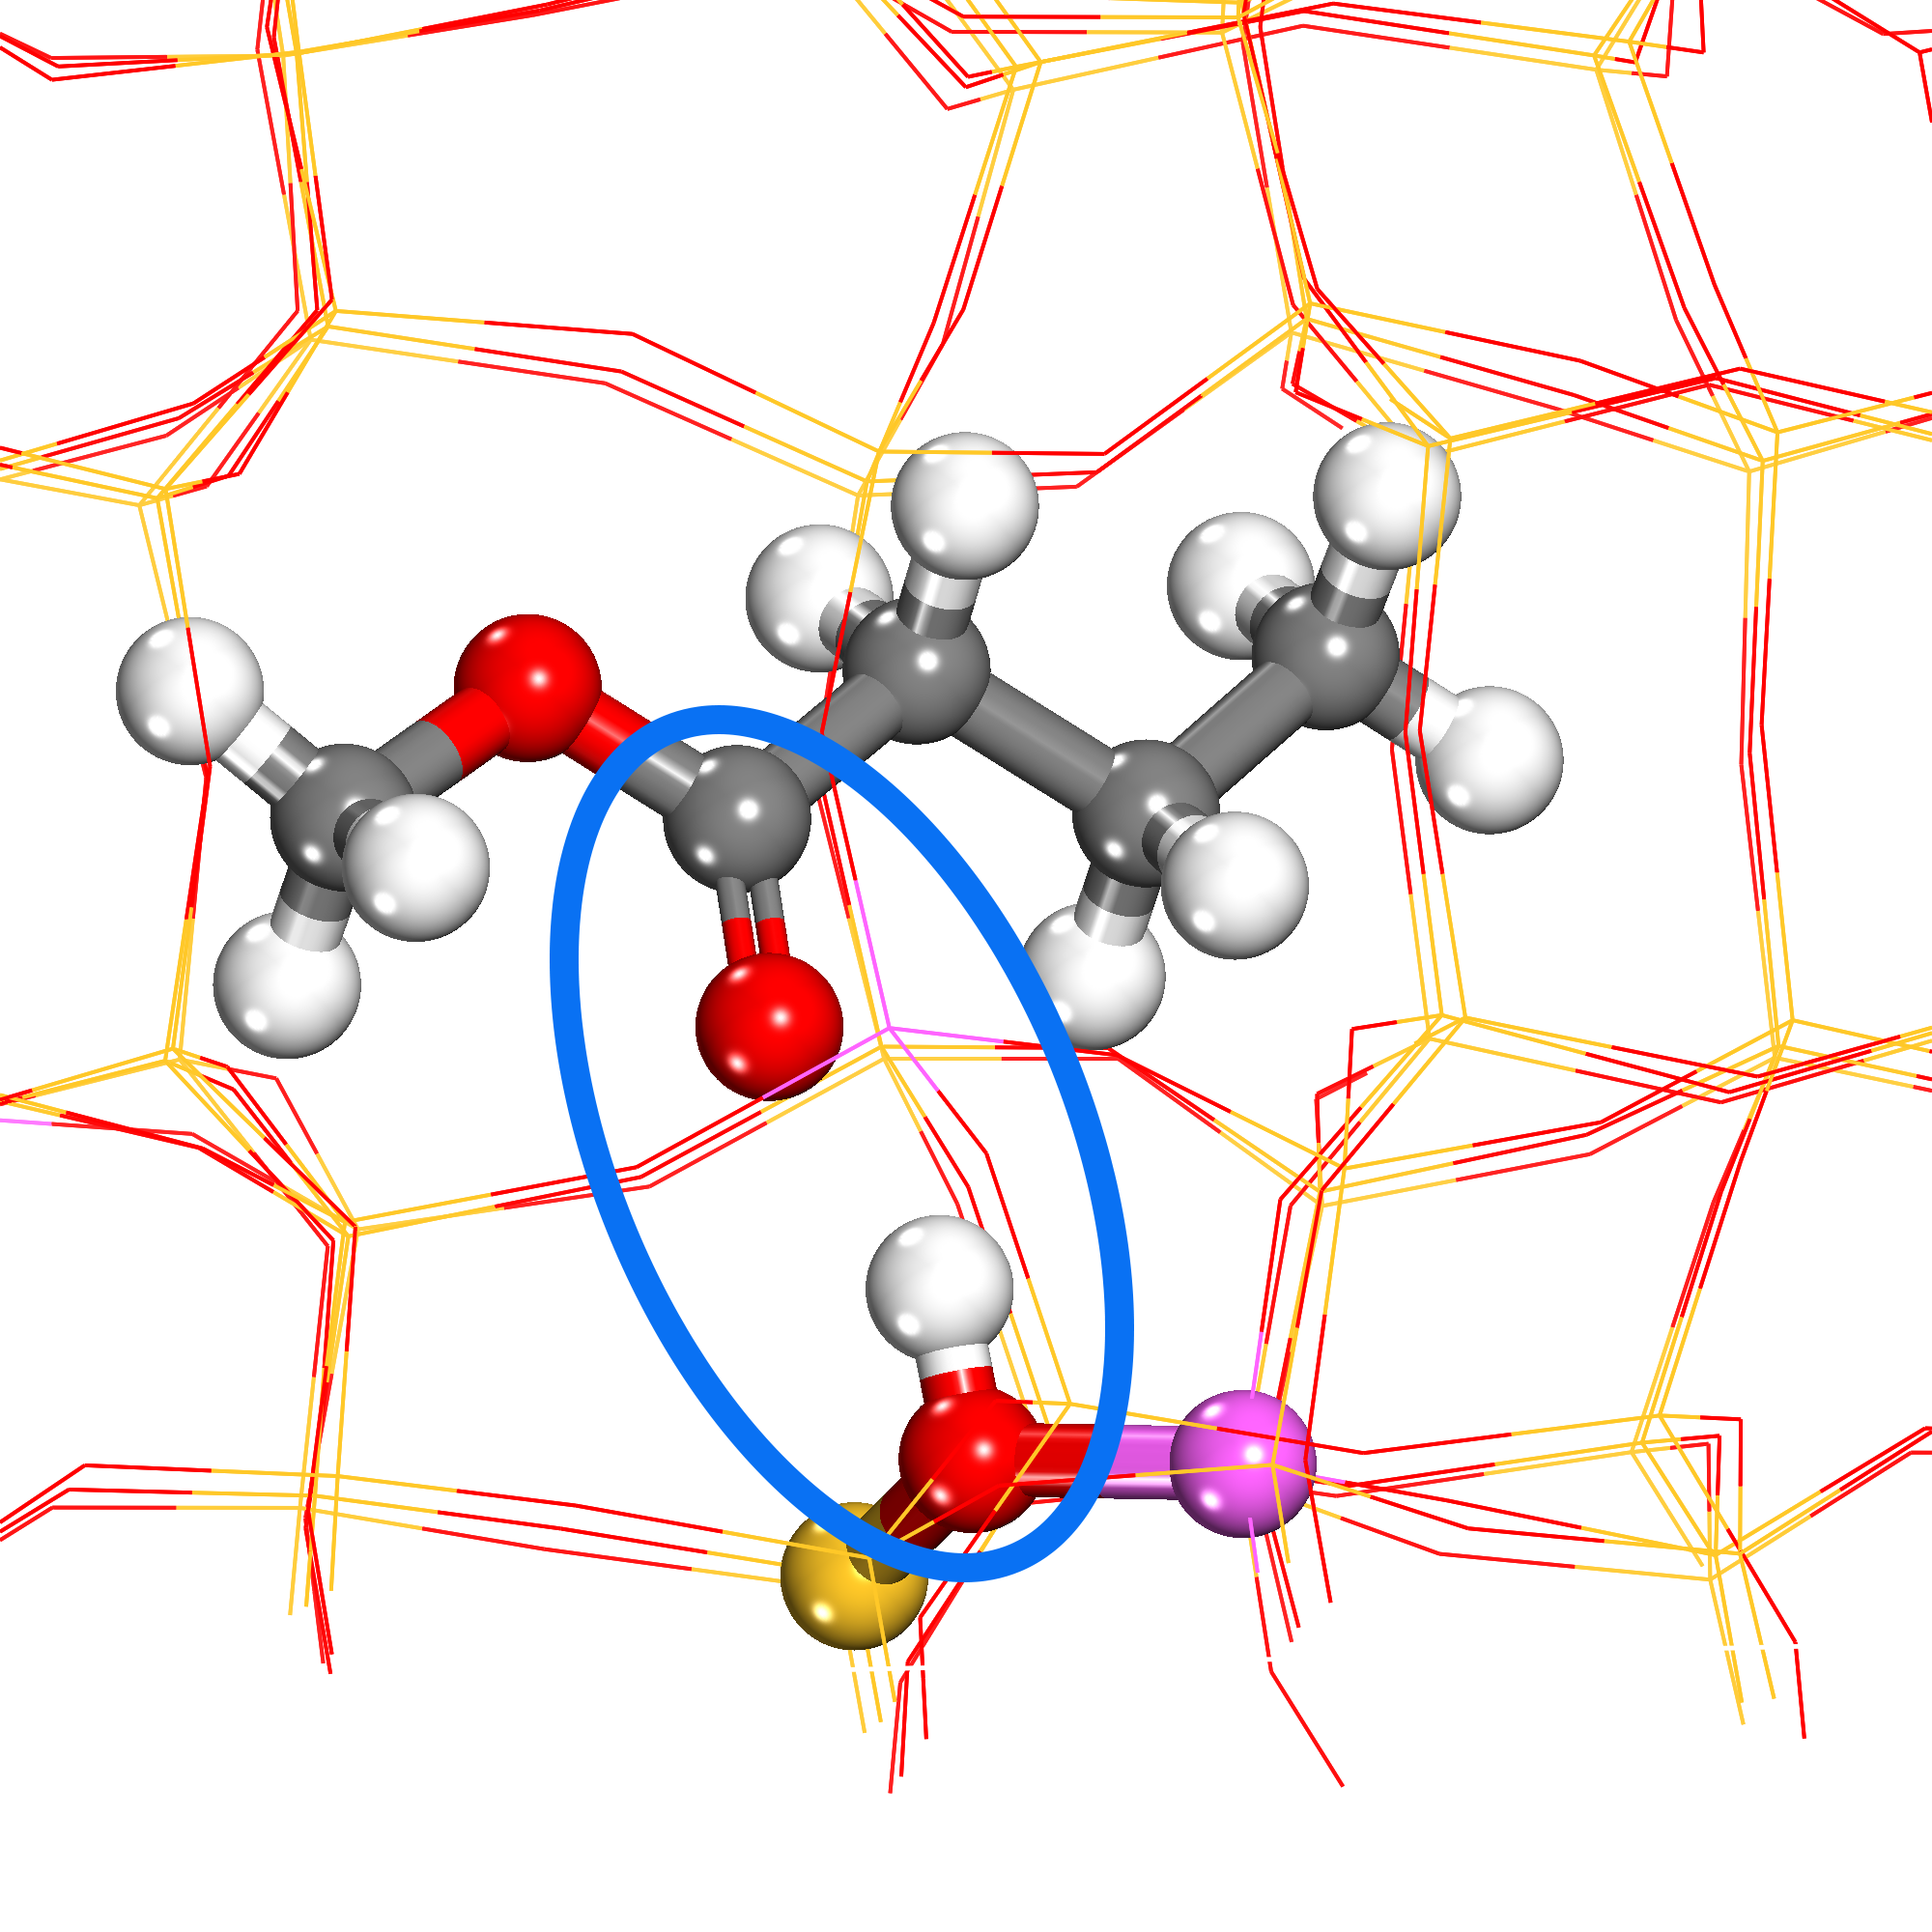
\includegraphics[width=2.7in]{figure/Adsorption/loaction.png}
    %\caption{fig1}
    \label{fig:L1}
    \end{minipage}%
    }%
    \subfigure[丁烯酸甲酯与B位酸吸附构型图]{
    \begin{minipage}[t]{0.5\linewidth}
    \centering
    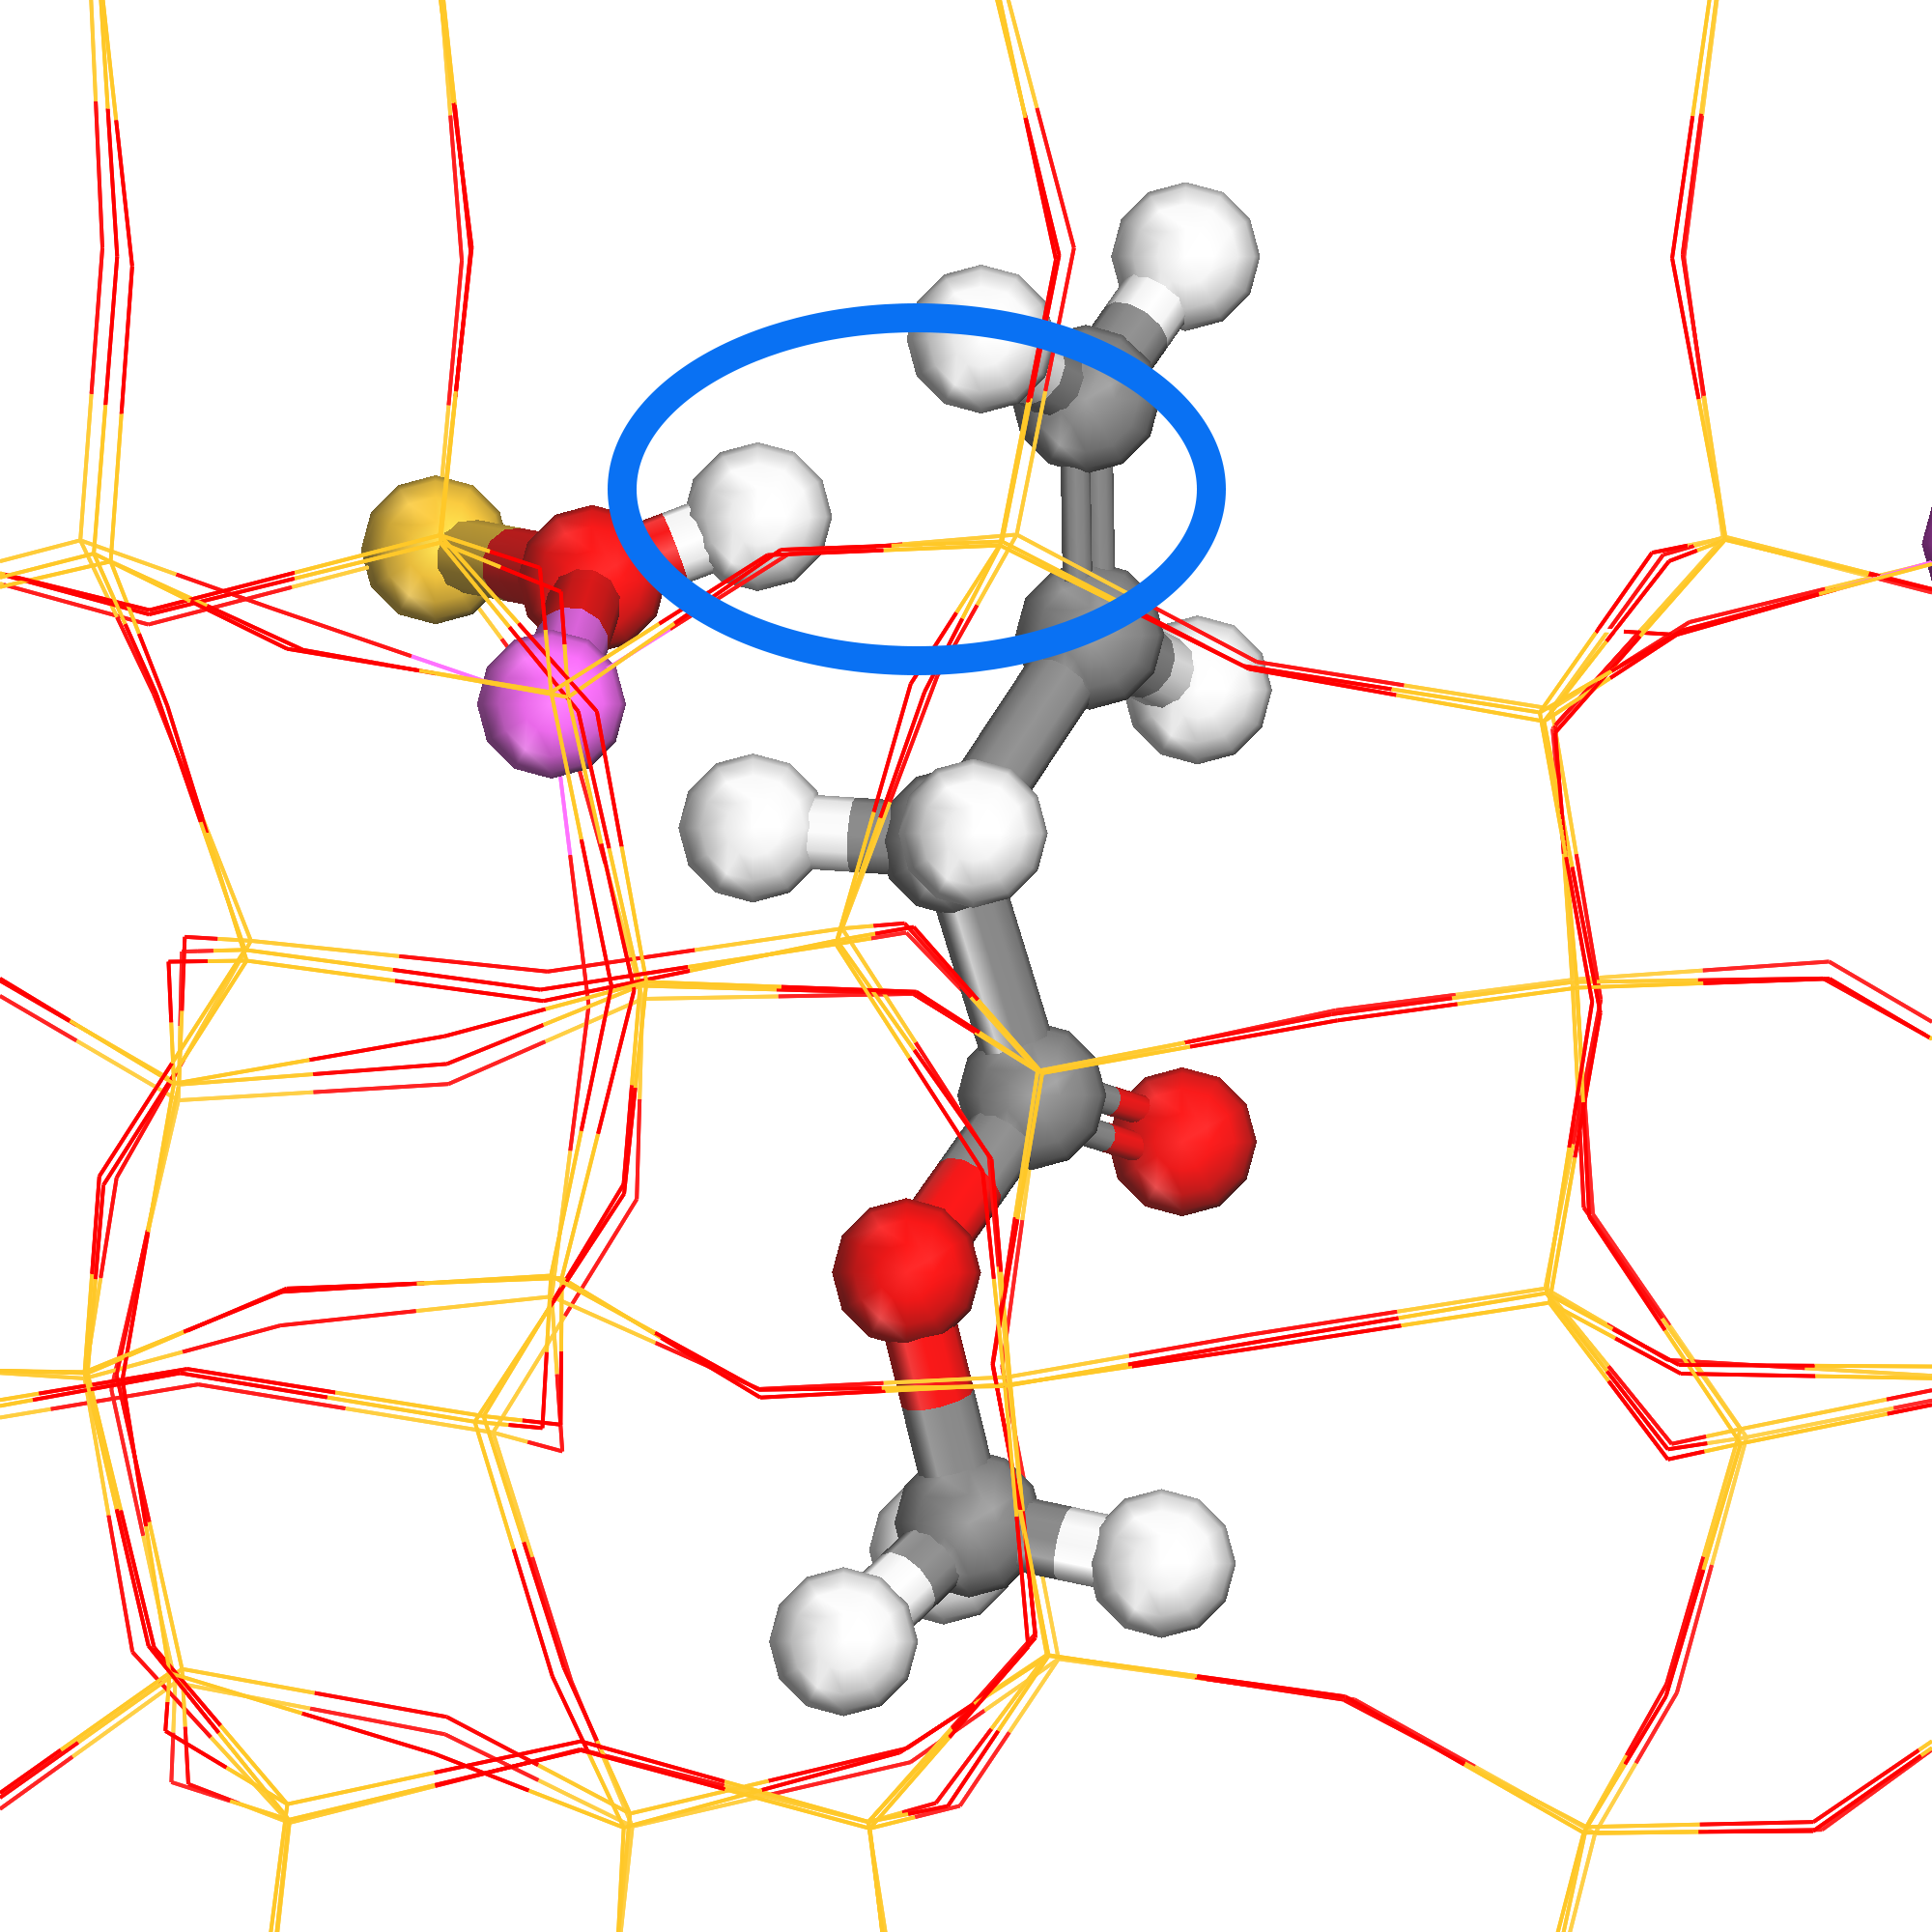
\includegraphics[width=2.7in]{figure/Adsorption/555.png}
    %\caption{fig2}
    \label{fig:L2}
    \end{minipage}%
    }%
    \caption{丁酸甲酯和丁烯酸甲酯与B位酸吸附构型图}
    \label{fig:L}
\end{figure}


\subsection{本章小结}
\par{本章采用GCMC(巨正则蒙特卡洛法),通过Materials Studio 8.0软件中的Sorption模块对丁酸甲酯等模型化合物在H-ZSM-5分子筛中进行了吸附模拟,得到以下结论:}
\begin{enumerate}
    \item 丁酸甲酯等模型化合物在微介孔H-ZSM-5分子筛的吸附等温线均属于\RNum{1}型等温线。随着孔径的增大,饱和吸附量减小,吸附平衡常数减小,单位质量分子筛的饱和吸附量先增大后减小,20Å介孔最大;随着温度的增大,饱和吸附量减小,吸附平衡常数减小;随着吸附分子极性增强,饱和吸附量增大,吸附平衡常数增大;随着吸附分子链长的增大,饱和吸附量减小,吸附平衡常数增大。
    \item 丁酸甲酯在微孔和介孔中的等量吸附热随压力(吸附量)的变化不同:在微孔中,随着压力的增大,等量吸附热以增量逐渐减小的方式增大,最后趋于最大值,而随着吸附量的增大,等量吸附热线性增大;在介孔中,随着压力或吸附量的增大,等量吸附热先增大再减小,有一个极大值。随着孔径的增大,相同压力下的等量吸附热减小。随着温度的增加,微孔介孔的等量吸附热都减小,在介孔中的等量吸附热最大值对应的压力几乎不变。在介孔中,随着温度的增加,孔径越大,等量吸附热最大值所对应的吸附量变化越小。
    \item 通过吸附构型图,可以发现丁酸甲酯优先吸附在活性吸附位(B位酸)处,并分布在交叉孔道旁,B位酸与双键氧形成氢键,随着压力的增大,丁酸甲酯在交叉孔道和直孔道都有吸附。丁烯酸甲酯中的双键与B位酸形成 π 配位超分子复合物。
\end{enumerate}

	%扩散
	\newpage
\section{脂肪酸甲酯在H-ZSM-5分子筛上的扩散}
\par{目前通过实验测量吸附分子在分子筛中的扩散系数是非常有挑战性的,因为很难将扩散与反应分离,扩散系数只能在相对低温下测量。虽然在任何期望温度下的扩散系数可以在确定指前因子和活化能后根据阿伦尼乌斯方程计算,但从较窄的低温范围得出的这些参数再外推到脂肪酸甲酯催化裂解的高温时可能会产生显著的误差\cite{bu2018diffusion}。}
\par{所以本章使用Materials Studio 8.0软件的Sorption模块和Forcite模块,进行了动力学模拟。主要计算了模型化合物丁酸甲酯在微介孔H-ZSM-5分子筛上的扩散系数。}
\subsection{Sorption 参数设置}\label{Sorption 扩散参数设置}
\par{本节使用Forcite模块与Sorption模块进行动力学模拟,相关参数设置如下:}
\begin{enumerate}
    \item 应用Sorption模块中的固定压力(Fixed Pressure)功能计算在温度673K和压力100kPa下,丁酸甲酯在不同孔径大小的分子筛的饱和吸附量,参数设置和 \ref{Sorption 参数设置} 所设参数一样。这样可以保证是在相同温度和压力下进行的比较。
    \item 应用Sorption模块中的固定吸附量(Fixed Loading)功能和手动放置吸附分子模型到介孔内的方法,分别在H-ZSM-5分子筛中负载对应饱和吸附量的分子个数,其余参数与 \ref{Sorption 参数设置} 相同。
    \item 对负载吸附分子的结构用 Forcite模块进行结构优化(Geometry Optimization)和模拟退火(Anneal),参数设置和 \ref{Forcite 参数设置} 一样。
    \item 然后对负载吸附分子的结构用Forcite 模块的Dynamics功能进行动力学模拟,采用NVT系综,随机给予初始速度,温度选择673K,模拟步长为1fs,模拟步数为100000,总体模拟时间100ps,每5000步输出一次图像用于分析扩散结果。
    \item 将上一步的结果再次进行Forcite Dynamics模拟,采用NVE系综,采用当前速度,模拟步长为1fs,模拟步数为400000,总体模拟时间400ps,每500步输出一次图像用于分析扩散结果。
\end{enumerate}

\subsection{模型验证}
\par{为了验证本文采用的计算扩散系数的方法和参数的正确性,本文将模拟计算出的正己烷分子在不同温度、不同孔径下的H-ZSM-5 分子筛的扩散系数的结果和文献\cite{bu2018diffusion}实验得到的结果相对比,模拟参数按照上文的参数设置。对比结果如\reftab{tab:C6}所示。采用 \ref{分子动力学} 所讲述的斯托克斯 - 爱因斯坦方程计算扩散系数。}
\begin{equation}
    D=\frac{1}{6 N} \lim _{x \rightarrow \infty} \frac{d}{d t} \sum_{i=1}^{N}\left\langle|r(t)-r(0)|^{2}\right\rangle
\end{equation}
\par{式中:$N$表示吸附分子总的数量;$r(0)$表示吸附分子质心的初始位置坐标;$r(t)$表示吸附分子在时间$t$时的质心坐标;$\left\langle|r(t)-r(0)|^{2}\right\rangle$表示扩散分子均方位移(MSD)的系综平均。}
\par{吸附分子在扩散过程中的均方位移可以直接从Materials Studio 8.0软件分析得出。以正己烷在60Å介孔H-ZSM-5分子筛的扩散为例,其均方位移随时间的变化曲线如\reffig{fig:C6}所示。}
\begin{figure}[H]
    \centering
        \includegraphics[width=0.5\linewidth]{figure/Diffusion/C6.pdf}
    \caption{正己烷均方位移随时间变化曲线图}
    \label{fig:C6}
\end{figure}
\par{从\reffig{fig:C6}中看出,MSD曲线大致为线性,曲线刚开始为对数形式,后半部分为直线,符合 \ref{分子动力学} 中文献所描述的MSD曲线的特点。所以根据斯托克斯 - 爱因斯坦方程拟合计算直线部分的斜率,得到各个条件下的扩散系数,并与文献结果相对比,具体数值见\reftab{tab:C6}。}
\begin{table}[H]
	\small
	\centering
	\caption{正己烷扩散系数模拟与实验数据对比表}
	\begin{tabular}{p{2.5cm}<{\centering}p{2cm}<{\centering}p{3cm}<{\centering}P{2.2}P{2.5}}
        \toprule
        孔径&\makecell{温度\\(K)}&\makecell{MSD曲线斜率\\(Å$^2$/ps)}&\multicolumn{1}{p{3cm}<{\centering}}{\makecell{计算扩散系数\\(×$10^{-10}$m$^2$/s)}}&\multicolumn{1}{p{3cm}<{\centering}}{\makecell{实验扩散系数\\(×$10^{-10}$m$^2$/s)}}\\
        \midrule
        \multirow{2}{*}{60Å介孔}&300&0.0795&13.25&12.4±0.5\\
        &400&0.0909&15.15&18.3±2.5\\
        \hline
        20Å介孔&300&0.0069&1.15&1.4±0.3\\
		\bottomrule
	\end{tabular}
	\label{tab:C6}
\end{table}
\par{由\reftab{tab:C6}可知,计算得到的结果和实验结果非常吻合,均处在误差范围内,所以本文采取的模型结构和力场是合理的。下面验证动力学模拟的参数设置是否合理。}
\par{本文对扩散模型进行了两次Forcite Dynamics模拟,首先在NVT系综模拟以确保系统温度达到平衡,在此基础下进行的NVE系综模拟时,体系温度会维持在一个相对恒定的水平。\reffig{fig:Temperature}为300k下正己烷在NVE系综扩散模拟中体系温度随着时间的变化。由图可知,己烷分子在整个动力学模拟过程中体系温度均处于较为恒定(300k)的状态,虽然有波动,但相对误差并未超过5\%,总体处于一个稳定范围。因此在模拟过程中,体系处在动力学平衡状态。}
\begin{figure}[H]
    \centering
        \includegraphics[height=0.5\textwidth]{figure/Diffusion/Temperature.pdf}
    \caption{正己烷分子在动力学模拟时的温度随时间变化图}
    \label{fig:Temperature}
\end{figure}
\subsection{模拟结果}
\par{本节主要分析了丁酸甲酯在不同孔径的分子筛内的扩散情况,包括了丁酸甲酯在介孔内的扩散、从介孔到微孔的扩散,在微孔内的扩散。}

\subsubsection{丁酸甲酯在介孔内的扩散}
\par{本小节主要讨论了丁酸甲酯在微孔和介孔中的扩散情况,说明了介孔对吸附分子扩散系数的影响。}
\par{首先先将丁酸甲酯放置在微孔和介孔中:用固定吸附并结构优化的方式将丁酸甲酯放置到微孔中;用手动放置并结构优化的方式将丁酸甲酯放置到介孔中。放置的分子个数由在673K、100kPa参数条件下的固定压力功能算出,分别为63、42和90个。以分子筛的C方向为例,如\reffig{fig:MMM}所示。}

\begin{figure}[H]
    \centering

    \subfigure[微孔]{
    \begin{minipage}[t]{0.3333\linewidth}
    \centering
    \includegraphics[width=2in]{figure/Diffusion/1MM.png}
    %\caption{fig1}
    \end{minipage}%
    }%
    \subfigure[20Å介孔]{
    \begin{minipage}[t]{0.3333\linewidth}
    \centering
    \includegraphics[width=2in]{figure/Diffusion/1M20.png}
    %\caption{fig2}
    \end{minipage}%
    }%
    \subfigure[60Å介孔]{
    \begin{minipage}[t]{0.3333\linewidth}
    \centering
    \includegraphics[width=2in]{figure/Diffusion/1M60.png}
    %\caption{fig2}
    \end{minipage}%
    }%
    \caption{丁酸甲酯在微孔和介孔内动力学模拟的初始位置示意图}
    \label{fig:MMM}
\end{figure}

\par{然后采用Forcite模块先后进行NVT和NVE系综的动力学模拟,设置参数如 \ref{Sorption 扩散参数设置} 所示,得到了丁酸甲酯在微介孔的均方位移随时间的变化曲线,如\reffig{fig:MSDd}所示。}
\begin{figure}[H]
    \centering

    \subfigure[微孔]{
    \begin{minipage}[t]{0.3333\linewidth}
    \centering
    \includegraphics[width=2in]{figure/Diffusion/MSDMM.pdf}
    \end{minipage}%
    }%
    \subfigure[20Å介孔]{
    \begin{minipage}[t]{0.3333\linewidth}
    \centering
    \includegraphics[width=2in]{figure/Diffusion/MSDM20.pdf}
    %\caption{fig2}
    \end{minipage}%
    }%
    \subfigure[60Å介孔]{
    \begin{minipage}[t]{0.3333\linewidth}
    \centering
    \includegraphics[width=2in]{figure/Diffusion/MSDM60.pdf}
    %\caption{fig2}
    \end{minipage}%
    }%
    \caption{丁酸甲酯在不同孔径H-ZSM-5分子筛的MSD vs. Time图}
    \label{fig:MSDd}
\end{figure}
\par{从\reffig{fig:MSDd}中看出,丁酸甲酯在不同孔径下的MSD曲线大致为线性,满足斯托克斯 - 爱因斯坦方程。根据 \ref{分子动力学} 中斯托克斯 - 爱因斯坦方程计算出在微介孔的扩散系数,具体数值见\reftab{tab:MSD}。}

\begin{table}[H]
	\small
	\centering
	\caption{丁酸甲酯在不同孔径H-ZSM-5分子筛中的扩散系数对比表}
	\begin{tabular}{p{2.5cm}<{\centering}P{2.4}P{3.4}p{2.5cm}<{\centering}P{4.2}}
        \toprule
        孔径&\multicolumn{1}{p{2.5cm}<{\centering}}{\makecell{斜率\\(Å$^2$/ps)}}&\multicolumn{1}{p{2.5cm}<{\centering}}{\makecell{截距\\(Å$^2$)}}&R$^2$&\multicolumn{1}{p{4cm}<{\centering}}{\makecell{扩散系数\\(×$10^{-10}$m$^2$/s)}}\\
        \midrule
        微孔&0.1514&5.5047&0.9613&25.23\\
        介孔20Å&13.7192&57.0054&0.9855&2286.53\\
        介孔60Å&32.7761&187.6688&0.9967&5462.68\\
        \bottomrule
	\end{tabular}
	\label{tab:MSD}
\end{table}
\par{由\reftab{tab:MSD}可知在催化裂化反应条件下,模型化合物丁酸甲酯在不同孔径的H-ZSM-5分子筛中的扩散能力为60Å介孔> 20Å介孔$\gg$微孔的扩散速率。与微孔H-ZSM-5 相比,在20Å 介孔中测量的扩散系数增加了2个数量级。然而,增加介孔H-ZSM-5 的孔径对扩散的影响不大,随着孔径从20Å增加到60Å,计算得到的扩散系数仅增加1.4倍。}

\subsubsection{丁酸甲酯从介孔到微孔的扩散}
\par{本小节主要讨论了丁酸甲酯从介孔孔道到微孔孔道的情况。}
\par{微孔分子筛的孔径大小通过其限制作用,基本上可以影响吸附分子的扩散,从而影响吸附分子的取向。比如Bu\cite{bu2016diffusion}证明了对二甲苯分子主要是平行于直孔道扩散的,因为其最长主轴的长度(9.1Å)大于微孔H-ZSM-5分子筛相对较小的孔径。而本文的丁酸甲酯的最长主轴的长度(7.8Å)也大于H-ZSM-5分子筛的孔径大小,所以丁酸甲酯必须以一定的取向才能进入微孔,否则将会被分子筛弹开。以60Å介孔为例,以一帧5ps的速度,\reffig{fig:MSDa}展示了扩散刚开始的35ps这段时间内丁酸甲酯的运动轨迹。}
\begin{figure}[H]
    \centering

    \subfigure[0ps]{
    \begin{minipage}[t]{0.25\linewidth}
    \centering
    \includegraphics[width=1.35in]{figure/Diffusion/1.png}
    \end{minipage}%
    }%
    \subfigure[5ps]{
    \begin{minipage}[t]{0.25\linewidth}
    \centering
    \includegraphics[width=1.35in]{figure/Diffusion/2.png}
    %\caption{fig2}
    \end{minipage}%
    }%
    \subfigure[10ps]{
    \begin{minipage}[t]{0.25\linewidth}
    \centering
    \includegraphics[width=1.35in]{figure/Diffusion/3.png}
    %\caption{fig2}
    \end{minipage}%
    }%
    \subfigure[15ps]{
    \begin{minipage}[t]{0.25\linewidth}
    \centering
    \includegraphics[width=1.35in]{figure/Diffusion/4.png}
    \end{minipage}%
    }%

    \subfigure[20ps]{
    \begin{minipage}[t]{0.25\linewidth}
    \centering
    \includegraphics[width=1.35in]{figure/Diffusion/5.png}
    %\caption{fig2}
    \end{minipage}%
    }%
    \subfigure[25ps]{
    \begin{minipage}[t]{0.25\linewidth}
    \centering
    \includegraphics[width=1.35in]{figure/Diffusion/6.png}
    %\caption{fig2}
    \end{minipage}%
    }%
    \subfigure[30ps]{
    \begin{minipage}[t]{0.25\linewidth}
    \centering
    \includegraphics[width=1.35in]{figure/Diffusion/7.png}
    \end{minipage}%
    }%
    \subfigure[35ps]{
    \begin{minipage}[t]{0.25\linewidth}
    \centering
    \includegraphics[width=1.35in]{figure/Diffusion/8.png}
    %\caption{fig2}
    \end{minipage}%
    }%

    \caption{丁酸甲酯在60Å介孔的H-ZSM-5分子筛的扩散轨迹随时间变化图}
    \label{fig:MSDa}
\end{figure}
\par{\reffig{fig:MSDa}清楚地展示了丁酸甲酯分子因为取向与微孔孔道方向不一样而被弹开的过程。而\reffig{fig:MSDf}展示了当丁酸甲酯的取向与微孔孔道一致时,丁酸甲酯顺利地进入A方向的之字形微孔内的过程。这进一步说明H-ZSM-5分子筛具有很高的择形性。}
\begin{figure}[H]
    \centering

    \subfigure[80ps]{
    \begin{minipage}[t]{0.25\linewidth}
    \centering
    \includegraphics[width=1.35in]{figure/Diffusion/1new.png}
    \end{minipage}%
    }%
    \subfigure[85ps]{
    \begin{minipage}[t]{0.25\linewidth}
    \centering
    \includegraphics[width=1.35in]{figure/Diffusion/2new.png}
    %\caption{fig2}
    \end{minipage}%
    }%
    \subfigure[90ps]{
    \begin{minipage}[t]{0.25\linewidth}
    \centering
    \includegraphics[width=1.35in]{figure/Diffusion/3new.png}
    %\caption{fig2}
    \end{minipage}%
    }%
    \subfigure[95ps]{
    \begin{minipage}[t]{0.25\linewidth}
    \centering
    \includegraphics[width=1.35in]{figure/Diffusion/4new.png}
    \end{minipage}%
    }%
    \caption{丁酸甲酯从介孔到微孔的扩散轨迹随时间变化图}
    \label{fig:MSDf}
\end{figure}

\subsubsection{丁酸甲酯在微孔内的扩散}
\par{本小节主要讨论了丁酸甲酯进入微孔内的情况。}
\par{为了更好地说明吸附分子从介孔进入微孔后,吸附分子在微孔内的扩散情况,本文将丁酸甲酯用Sorption模块的固定吸附的方式将丁酸甲酯固定在微孔内,并与微孔分子筛的结果进行对比。以分子筛的C方向为例,如\reffig{fig:MMe}所示}

\begin{figure}[H]
    \centering

    \subfigure[微孔]{
    \begin{minipage}[t]{0.3333\linewidth}
    \centering
    \includegraphics[width=1.8in]{figure/Diffusion/2MM.png}
    %\caption{fig1}
    \end{minipage}%
    }%
    \subfigure[20Å介孔]{
    \begin{minipage}[t]{0.3333\linewidth}
    \centering
    \includegraphics[width=1.8in]{figure/Diffusion/2M20.png}
    %\caption{fig2}
    \end{minipage}%
    }%
    \subfigure[60Å介孔]{
    \begin{minipage}[t]{0.3333\linewidth}
    \centering
    \includegraphics[width=1.8in]{figure/Diffusion/2M60.png}
    %\caption{fig2}
    \end{minipage}%
    }%
    \caption{丁酸甲酯在微孔内的初始位置示意图}
    \label{fig:MMe}
\end{figure}
\par{然后分别对各个体系进行动力学计算,温度选取为673K,模拟总时间位200ps,结果如\reffig{fig:MSDq}所示。丁酸甲酯无论是在20Å介孔的微孔内,还是在60Å介孔的微孔内,它的均方位移随时间变化的曲线的斜率几乎和在微孔分子筛内的一样大,具体的拟合结果如\reftab{tab:MMa}所示。}
\par{由\reftab{tab:MMa}可知,在20Å介孔和60Å介孔中的扩散系数几乎一样大,只比在微孔中的扩散系数大9.4\%,这说明在丁酸甲酯进入微孔后的前200ps内,丁酸甲酯几乎没有从微孔进入介孔,而是在微孔内做着受限运动,这与从扩散轨迹得到的结论是一致的。但因为介孔中的活性吸附位和一般吸附位都临近介孔,所以丁酸甲酯受到的空间位阻与在微孔中的相对较小,所以扩散系数依然比在微孔中的大,这与温度对在微孔中的等量吸附热的影响比在介孔中的小的解释是一致的。}

\begin{figure}[H]
    \centering
        \includegraphics[width=0.5\textwidth]{figure/Diffusion/MSD.pdf}
    \caption{丁酸甲酯在不同孔径H-ZSM-5分子筛的微孔内的MSD vs. Time图}
    \label{fig:MSDq}
\end{figure}

\begin{table}[H]
	\small
	\centering
	\caption{丁酸甲酯在不同分子筛微孔中的扩散系数对比表}
	\begin{tabular}{p{2.5cm}<{\centering}p{3cm}<{\centering}p{3cm}<{\centering}P{2.2}}
        \toprule
        孔径&\makecell{MSD曲线斜率\\(Å$^2$/ps)}&R$^2$&\multicolumn{1}{p{3cm}<{\centering}}{\makecell{扩散系数\\(×$10^{-10}$m$^2$/s)}}\\
        \midrule
        微孔&0.1413&0.9773&23.55\\
        20Å介孔&0.1546&0.9729&25.77\\
        60Å介孔&0.1545&0.9777&25.75\\
		\bottomrule
	\end{tabular}
	\label{tab:MMa}
\end{table}




\subsection{本章小结}
\par{本章在673k(催化裂化温度)和100kPa(常压)下对丁酸甲酯分子在微介孔H-ZSM-5分子筛上的扩散进行了模拟,分析得到了丁酸甲酯的均方位移随时间的变化曲线,并根据斯托克斯 - 爱因斯坦方程计算得到在微孔、20Å介孔和60Å介孔分子筛中的扩散系数,得到了以下结论:}
\begin{enumerate}
    \item 丁酸甲酯扩散系数的大小顺序为60Å介孔> 20Å介孔$\gg$微孔,这个结果与实验结果一致\cite{christensen2003catalytic,meunier2012influence}。介孔 H-ZSM-5 分子筛相对于传统的微孔 H-ZSM-5 分子筛,具有着更高效的质量传递性质。但随着孔径的增大,孔径大小对扩散系数的影响变小:从微孔到20Å介孔,扩散系数增加了89.6倍;而从20Å介孔到60Å介孔,扩散系数只增加了1.4倍。
    \item 丁酸甲酯要从介孔进入微孔,取向和孔径方向必须一致,否者将会被分子筛弹开,这说明H-ZSM-5分子筛具有很高的择形性。
    \item 当丁酸甲酯进入微孔后,在介孔分子筛中的微孔的扩散系数只比在微孔中的大9.4\%,说明丁酸甲酯几乎不能再从微孔进入介孔。
\end{enumerate}

	%结论
	\section{结论}
\par{本文使用Materials Studio 8.0软件对脂肪酸甲酯在微介孔H-ZSM-5分子筛上的吸附扩散进行模拟,通过分析模型化合物的吸附扩散性能得到以下结论:}
\begin{enumerate}
    \item 丁酸甲酯等模型化合物在微介孔H-ZSM-5分子筛的吸附等温线均属于\RNum{1}型等温线。随着孔径的增大,饱和吸附量减小,吸附平衡常数减小,单位质量分子筛的饱和吸附量先增大后减小,20Å介孔的最大;随着温度的增大,饱和吸附量减小,吸附平衡常数减小;随着吸附分子极性增强,饱和吸附量增大,吸附平衡常数增大;随着吸附分子链长的增大,饱和吸附量减小,吸附平衡常数增大。
    \item 丁酸甲酯在微孔和介孔中的等量吸附热随压力(吸附量)的变化不同:在微孔中,随着压力的增大,等量吸附热以增量逐渐减小的方式增大,最后趋于最大值,而随着吸附量的增大,等量吸附热线性增大;在介孔中,随着压力或吸附量的增大,等量吸附热先增大再减小,有一个极大值。随着孔径的增大,相同压力下的等量吸附热减小。随着温度的增加,微孔介孔的等量吸附热都减小。
    \item 丁酸甲酯优先吸附在活性吸附位(B位酸)处,并分布在交叉孔道旁,B位酸与双键氧形成氢键,随着压力的增大,丁酸甲酯在交叉孔道和直孔道都有吸附。而丁烯酸甲酯中的双键与B位酸形成 π 配位超分子复合物。
    \item 丁酸甲酯扩散系数的大小顺序为60Å介孔> 20Å介孔$\gg$微孔,这个结果与实验结果一致。但随着孔径的增大,孔径大小对扩散系数的影响变小:从微孔到20Å介孔,扩散系数增加了89.6倍;而从20Å介孔到60Å介孔,扩散系数只增加了1.4倍。
\end{enumerate}
\par{介孔H-ZSM-5分子筛相比于微孔H-ZSM-5分子筛,单位质量下对脂肪酸甲酯的饱和吸附量增大,等量吸附热减小,扩散速率显著提高,吸附扩散性能增强。但介孔的孔径并不是越大越好,在单位质量的20Å介孔比在60Å介孔的饱和吸附量大,在60Å介孔中的扩散系数只比在20Å介孔的增加了1.8倍。}

	%致谢页
	\begin{thankpage}
\par{大学生活一晃而过,回首走过的岁月,心中倍感充实,当我写完这篇毕业论文的时候,有一种如释重负的感觉,感慨良多。}
\par{首先诚挚地感谢我的论文指导老师,刘熠斌老师。他在忙碌的教学工作中挤出时间来审查、修改我的论文。还有教过我的所有老师们,你们严谨细致、一丝不苟的作风一直是我学习中的榜样;你们循循善诱的教导和不拘一格的思路给予我无尽的启迪。}
\par{此外还要感谢李瑞英师姐以及实验室所有师兄师姐在我整个论文撰写以及模拟计算过程中提供的帮助和指导,这极大程度上解决了我在毕业论文过程中遇到的各类难题。}
\par{最后感谢家人在我大学本科四年学习生活上各方面的无私支持。}

\end{thankpage}

	%参考文献页
	\bibliography{Bibs/bibliography.bib}

%\begin{generalappendices}
%%\begin{appendices}
%	\section{Appendix 1}
%	\subsection{Some Appendix}
%	\lipsum[11]
%	\section{Appendix 2}
%	\subsection{Some Other Appendix}
%%\end{appendices}[toc, page, title, titletoc, header]
%\end{generalappendices}
\end{document}
